%%%%%%%%%%%%%%%%%%%%%%%%%%%%%%%%%%%%%%%%%%%%%%%%%%
%% Bachelor's & Master's Thesis Template        %%
%% Copyleft by Dawid Weiss & Marta Szachniuk    %%
%% Faculty of Computing and Telecommunication   %%
%% Poznan University of Technology, 2020        %%
%%%%%%%%%%%%%%%%%%%%%%%%%%%%%%%%%%%%%%%%%%%%%%%%%%

% Szkielet dla pracy Magisterskiej pisanej w języku polskim.

\documentclass[polish,a4paper,oneside]{ppfcmthesis}
\pagenumbering{arabic}

\usepackage[utf8]{inputenc}
\usepackage[OT4]{fontenc}
\usepackage{float}
\usepackage[inkscapelatex=false]{svg}
\usepackage{geometry}
\usepackage{graphicx}
\usepackage{tocloft}
\usepackage{msc}
\usepackage{pgfplots}
\usepackage{tikz}
\pgfplotsset{compat=1.17}
\usepackage{listings}

% Define custom colors
\definecolor{comment}{rgb}{0.5,0.5,0.5}
\definecolor{keyword}{rgb}{0.0,0.0,0.8}
\definecolor{string}{rgb}{0.8,0.0,0.0}

% Define Java language settings for listings
\lstdefinestyle{customjava}{
  language=Java,
  basicstyle=\ttfamily\footnotesize,
  keywordstyle=\color{keyword}\bfseries,
  commentstyle=\color{comment}\itshape,
  stringstyle=\color{string},
  numberstyle=\tiny\color{comment},
  stepnumber=1,
  numbers=left,
  numbersep=10pt,
  showspaces=false,
  showstringspaces=false,
  tabsize=4,
  breaklines=true,
  breakatwhitespace=false,
  escapeinside={(*@}{@*)}
}

\lstdefinestyle{yaml}{
     basicstyle=\color{blue}\footnotesize,
     rulecolor=\color{black},
     string=[s]{'}{'},
     stringstyle=\color{blue},
     comment=[l]{:},
     commentstyle=\color{black},
     morecomment=[l]{-}
 }

% Set the style for listings
\lstset{style=customjava}

%--------------------------------------
% Strona tytułowa
%--------------------------------------

% Autorzy pracy, jeśli jest ich więcej niż jeden
% wstaw między nimi separator \and
\author{% 
    Jan Biały \album{144334}}
\authortitle{inż.}

\title{Zarządzanie przydziałem zasobów w środowisku Metaverse}

% Your supervisor comes here.
\ppsupervisor{prof.~dr hab.~inż.~Anna Kobusińska} 

% Year of final submission (not graduation!)
\ppyear{2024}                                 

\begin{document}
\pagestyle{ppfcmthesis}%

% Front matter starts here
\pagestyle{empty}%
\maketitle\cleardoublepage%

%--------------------------------------
% Miejsce na kartę pracy dyplomowej
%--------------------------------------

\thispagestyle{empty}\vspace*{\fill}%
\begin{center}Tutaj będzie karta pracy dyplomowej;\\oryginał wstawiamy do wersji dla archiwum PP, w pozostałych kopiach wstawiamy ksero.\end{center}%
\vfill\cleardoublepage%

%--------------------------------------
% Spis treści
%--------------------------------------

\setcounter{tocdepth}{2}
\tableofcontents*
\cleardoublepage % Ensure TOC ends and we start fresh

%--------------------------------------
% Rozdziały
%--------------------------------------

% Reset the page numbering to Arabic numerals for the main content
\pagestyle{ppfcmthesis}

\input{chapters/01-streszczenie_abstrakt}
\chapter{Wstęp}

\subsubsection{Kontekst}
\subsubsection{Cel pracy}

Podstawowym celem pracy jest stworzenie protokołu doboru zasobów do zapotrzebowania klienta w środowisku rozproszonym.

\subsubsection{Zawartość kolejnych rozdziałów}


\chapter{Podstawy teoretyczne}
\section{Metaverse}


Metaverse to koncepcja w świecie technologicznym, która odnosi się do cyfrowego środowiska życia w którym konwencjonalne struktury społeczne ulegają zmianie. Jest to termin, który łączy w sobie koncepcje greckiego prefiksu „meta”, który oznacza „pełniejszy” lub „przekraczający”, oraz akronimu „Verse” oznaczającego „wszechświat”, który oznacza pojemnik czasoprzestrzenny. Idea metawersji została wprowadzona w powieści science fiction Neala Stephensona \definicja{Snow Crash} w 1992 roku. Szybki rozwój technologii takich jak blockchain, wirtualna (\english{Virtual Reality}) i rozszerzona (\english{Augmented Reality}) rzeczywistość, gry, sztuczna inteligencja i Internet Rzeczy \acronym{IoT} (\english{Internet Of Things}) sprawiły, że metawersja stała się jednym z najbardziej popularnych terminów w świecie technologii. Rozwiązania i usługi są opracowywane dla wirtualnych światów, aby umożliwić użytkownikom dobrą zabawę, inteligentne angażowanie się w otoczenie i nawiązywanie głębszych relacji z innymi użytkownikami \cite{metaverseAsAService}. 

\begin{figure}[h!]
    \centering
    \includesvg[width=0.7\textwidth]{images/metaverse/MetaverseInfographic.svg}
    \caption{Koncepcyjny widok metaverse\cite{metaverseUseCaseslee}}
    \label{fig:enter-label}
\end{figure}

Metaverse jako wirtualny świat  wchodzący w interakcję ze światem rzeczywistym i śwaitem ludzkim. Interakcja ta została przedstawiona na ryskunku \ref{abstractMetaverseArchitectureHumanVirtualPhisical}. Metaverse jest uważany za idealne ucieleśnienie Internetu w przyszłości. Zintegrowany z zaawansowanymi technologiami, metawersja może być wirtualną przestrzenią wzbogaconą o rzeczywistość fizyczną. Użytkownicy są połączeni w wirtualnym wszechświecie we wciągającej interakcji i są ze sobą połączeni w celu prowadzenia działań społecznych. Odkąd koncepcja metaverse została zaproponowana w filmie naukowym \definicja{Snow Crash}, ludzie są stopniowo przyzwyczajają się do wirtualnych i internetowych aktywności zamiast w fizyczny i konwencjonalny sposób. Odkąd zaproponowano Przemysł 4.0, produkcja przemysłowa przekształca się w kierunku inteligentnej produkcji zwłaszcza w całym cyklu życia produktu, obejmującym badania i rozwój, produkcję, testy i eksperymenty, sprzedaż i transakcje oraz usługi i konserwację. Dzięki zaawansowanym technologiom informacyjno-komunikacyjnym, technologiom rozszerzonej rzeczywistości i sztucznej inteligencji, inteligentna produkcja jest wspierana przez wyższą wydajność produkcji i zwiększoną wirtualną interaktywność użytkowników. Ponadto, jako nowy paradygmat produkcji, produkcja w chmurze wygodnie zapewnia użytkownikom usługi na żądanie. Rozproszone zasoby produkcyjne są wirtualizowane i zarządzane w ujednolicony, zoptymalizowany i konfigurowalny sposób, umożliwiając wysoce wirtualną współpracę i innowacyjną produkcję\cite{industrialMetaverseForSmartManufacturing}. 

\begin{figure}[htbp!]
    \centering
    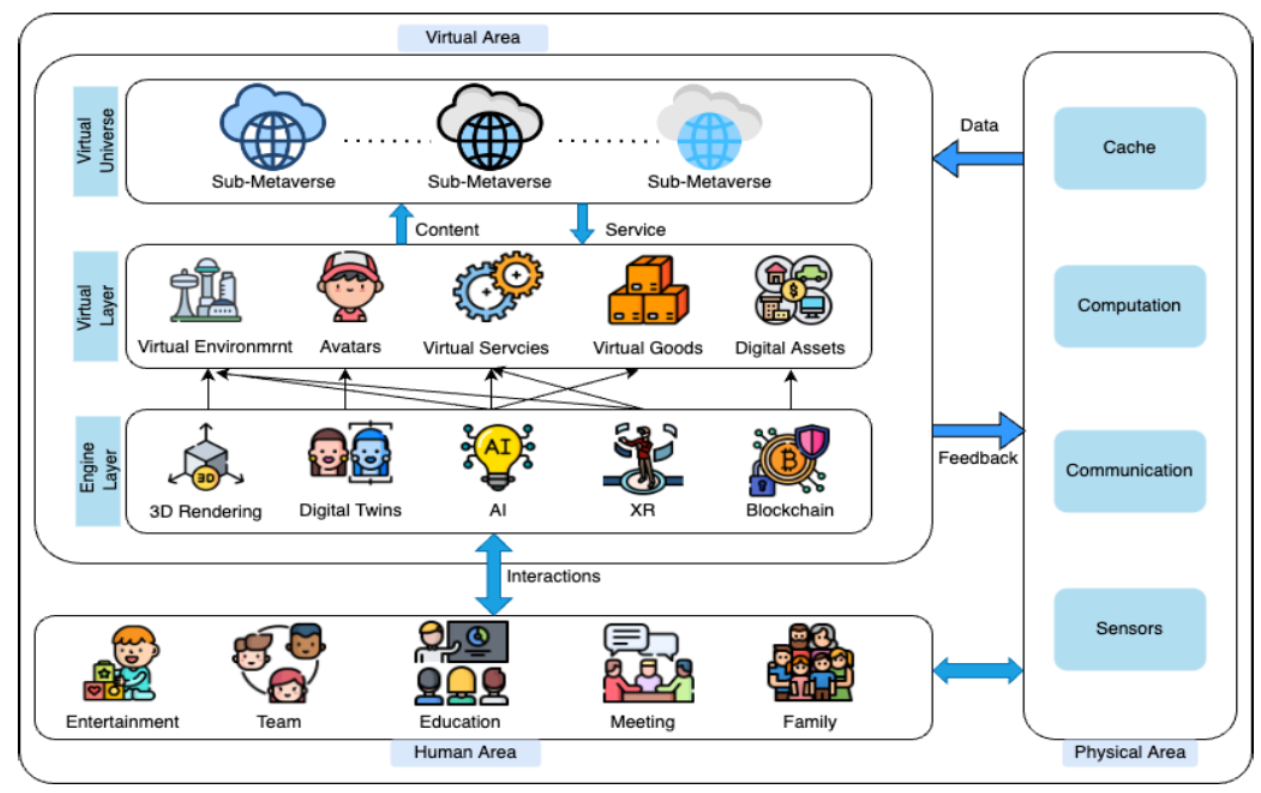
\includegraphics[width=\textwidth]{images/metaverse/metaverseAbstractArchitecture.png}
    \caption{Architektura Metaverse realizuje interakcje pomiędzy obszarem wirtualnym, obszarem ludzkim i obszarem fizycznym\cite{aSurveyofMobileEdgeComputingForMetaverse}}
    \label{abstractMetaverseArchitectureHumanVirtualPhisical}
\end{figure}

Kluczowe cechy metaverse:

\begin{itemize}
    \item Trwałość oznacza, istnienie niezależnie od fizycznej obecności użytkownika\cite{metaverseAFullDive}.
    \item Nieskończoność obsługiwanie niezliczonej liczby użytkowników i światów VR\cite{metaverseAFullDive}.
    \item Samowystarczalność oznacza, że użytkownicy mogą zarabiać w Metaverse i płacić za swoją użyteczność\cite{metaverseAFullDive}.
    \item Interoperacyjność pomaga użytkownikom przenosić ich wirtualne przedmioty, w tym awatary, z jednego projektu Metaverse do drugiego\cite{metaverseAFullDive}.
    \item Czas rzeczywisty pozwala użytkownikom cieszyć się doświadczeniami na żywo\cite{metaverseAFullDive}.
\end{itemize}


Metaverse ma być wciągającym wirtualnym światem, który płynnie łączy sferę fizyczną i cyfrową, umożliwiając użytkownikom interakcję, współpracę i angażowanie się w szereg działań we wspólnym wirtualnym środowisku. U podstaw tej rewolucyjnej koncepcji leży solidna infrastruktura, która służy jako szkielet, ułatwiając płynną łączność i interoperacyjność. Infrastruktura metaverse to ewoluująca, złożona sieć wzajemnie połączonych technologii, protokołów i ram, które współpracują ze sobą w celu stworzenia jednolitego i spójnego wirtualnego wszechświata\cite{metaverseInfrastructureIEEE}.

Infrastruktura ta obejmuje szeroką gamę komponentów, w tym szybkie sieci, potężne zasoby obliczeniowe, zaawansowane urządzenia sprzętowe i najnowocześniejsze platformy oprogramowania. Wykorzystuje ona najnowsze osiągnięcia w takich dziedzinach jak rzeczywistość wirtualna, rzeczywistość rozszerzona, blockchain i zdecentralizowane przetwarzanie danych, aby zapewnić wciągające i bezpieczne doświadczenie metawersji użytkownikom na całym świecie\cite{metaverseInfrastructureIEEE}.

\subsubsection{Architektura sieci w metawersji}

Architektura sieci w metaverse została zaprojektowana tak, aby wspierać płynne interakcje i komunikację w czasie rzeczywistym, umożliwiając użytkownikom angażowanie się w różne działania bez doświadczania opóźnień lub rozłączeń. Wykorzystuje ona zaawansowane protokoły i technologie sieciowe, które priorytetowo traktują niskie opóźnienia, wysoką przepustowość i wydajny transfer danych\cite{metaverseInfrastructureIEEE}.

Zdecentralizowane sieci odgrywają kluczową rolę w zwiększaniu łączności metaverse. Wykorzystując technologię blockchain i sieci peer-to-peer, infrastruktura metaverse ma na celu zmniejszenie zapotrzebowania na centralizacje zarządców lub pośredników. Takie podejście może zapewnić odporność, przejrzystość i demokratyczne zarządzanie, umożliwiając użytkownikom udział w rozwoju metawersji i procesach decyzyjnych\cite{metaverseInfrastructureIEEE}.

Przesyłanie danych i zarządzanie nimi w ramach infrastruktury metaverse jest ułatwione dzięki połączeniu tradycyjnych technologii sieciowych i nowych systemów rozproszonych. Szybkie sieci światłowodowe i łączność bezprzewodowa 5G/6G zapewniają przepustowość niezbędną do przesyłania bogatych treści multimedialnych i strumieni danych w czasie rzeczywistym. Jednocześnie zdecentralizowane rozwiązania pamięci masowej, takie jak rozproszone systemy plików i InterPlanetary File System \akronim{IPFS}, zapewniają bezpieczne i redundantne przechowywanie danych, umożliwiając efektywny dostęp do zasobów cyfrowych i ich wyszukiwania\cite{metaverseInfrastructureIEEE}.

Technologie przetwarzania na krawędzi (\english{Edge Computing}) mogą znacząco przyczynić się do zwiększenia wydajności infrastruktury metaverse. Przybliżając zasoby obliczeniowe do urządzeń brzegowych (takich jak zestawy słuchawkowe VR i okulary AR), przetwarzanie brzegowe zmniejsza opóźnienia i poprawia szybkość reakcji, zwiększając ogólne wrażenia użytkownika. Podejście to odciąża również scentralizowane serwery od zadań przetwarzania, rozkładając obciążenie obliczeniowe na całą sieć i zapewniając skalowalność w miarę wzrostu rozmiaru i złożoności metaverse\cite{metaverseInfrastructureIEEE}.

Technologie blockchain mogą odgrywać kluczową rolę w zwiększaniu bezpieczeństwa sieci w metawersji. Wykorzystując zdecentralizowane mechanizmy konsensusu i protokoły kryptograficzne, blockchain zapewnia integralność i niezmienność danych, chroniąc przed manipulacją i nieautoryzowanym dostępem. Dodatkowo, inteligentne kontrakty ułatwiają bezpieczne i przejrzyste interakcje, automatyzując złożone procesy i umożliwiając transakcje bez zaufania w ramach architektury metaverse i modelowania 3D\cite{metaverseInfrastructureIEEE}.

\subsubsection{Wymagania sprzętowe dla metawersji}

Aby uzyskać dostęp i w pełni doświadczyć metawersji, użytkownicy będą potrzebować specjalistycznego sprzętu, który może obsługiwać wciągające środowiska wirtualne i płynne interakcje. Podstawą tych wymagań sprzętowych są urządzenia komputerowe, takie jak komputery stacjonarne, konsole do gier lub wyspecjalizowane stacje robocze do rozwoju metaverse. Urządzenia te muszą posiadać wystarczającą moc obliczeniową, możliwości graficzne i zasoby pamięci, aby renderować szczegółowe środowiska 3D i obsługiwać złożone symulacje technologii metaverse\cite{metaverseInfrastructureIEEE}.

Infrastruktura metaverse w dużym stopniu wykorzystuje urządzenia rzeczywistości rozszerzonej i wirtualnej, aby zapewnić użytkownikom wciągające wrażenia. Zestawy VR, takie jak Oculus Rift, HTC Vive i PlayStation VR, przenoszą użytkowników do w pełni zrealizowanych wirtualnych światów, umożliwiając im interakcję z cyfrowymi obiektami i awatarami tak, jakby były prawdziwe. Urządzenia AR, takie jak Microsoft HoloLens i Magic Leap One, płynnie łączą elementy cyfrowe ze światem fizycznym, umożliwiając użytkownikom rozszerzenie otoczenia o wirtualne nakładki i interaktywne interfejsy\cite{metaverseInfrastructureIEEE}.

Zaawansowane jednostki przetwarzające, w tym wysokowydajne procesory graficzne \akronim{GPU} (\english{Graphics Processing Unit}) i wyspecjalizowane akceleratory, odgrywają kluczową rolę w zwiększaniu doznań płynących z metaverse. Komponenty te są odpowiedzialne za renderowanie złożonych środowisk 3D, symulację fizyki i przetwarzanie ogromnych ilości danych w czasie rzeczywistym. Dodatkowo, integracja sztucznej inteligencji i technologii uczenia maszynowego w infrastrukturze metaverse wymaga potężnych zasobów obliczeniowych, aby umożliwić inteligentne interakcje, przetwarzanie języka naturalnego i realistyczne awatary\cite{metaverseInfrastructureIEEE}.

Wraz z ciągłym rozwojem technologii, infrastruktura metaverse dostosowuje się do nowych technologii, które mogą jeszcze bardziej poprawić wrażenia użytkownika. Przykładowo, rozwój interfejsów mózg-komputer \akronim{BCI} (\english{Brain-Computer Interface}) i haptycznych urządzeń sprzężenia zwrotnego może zrewolucjonizować sposób interakcji użytkowników ze środowiskami wirtualnymi, umożliwiając bardziej intuicyjne i wciągające doświadczenia. Co więcej, postępy w dziedzinie obliczeń kwantowych i przetwarzania fotonicznego mogą potencjalnie zrewolucjonizować metawersję, zapewniając bezprecedensową moc obliczeniową a co za tym idzie możliwości przetwarzania danych\cite{metaverseInfrastructureIEEE}.

\subsubsection{Transakcje w metawersji}

Wirtualne waluty i technologia blockchain znajdują się w czołówce, jeśli chodzi o ułatwianie transakcji w metaverse. Te cyfrowe aktywa, często określane jako kryptowaluty lub tokeny, mogą służyć jako podstawowy środek wymiany towarów, usług i wirtualnych aktywów w wirtualnym środowisku metaverse. Wykorzystując zdecentralizowany i bezpieczny charakter technologii blockchain, te wirtualne waluty umożliwiają płynne, przejrzyste i pozbawione zaufania transakcje, eliminując potrzebę pośredników i zmniejszając koszty transakcji\cite{metaverseInfrastructureIEEE}.

Inteligentne kontrakty, które są samowykonalnymi umowami zakodowanymi w sieciach blockchain, mogą odgrywać kluczową rolę w automatyzacji i zabezpieczaniu transakcji w metaverse. Kontrakty te definiują zasady i warunki różnych umów, takich jak transfery aktywów, umowy o świadczenie usług i rozliczenia finansowe. Po wdrożeniu, inteligentne kontrakty wykonują się automatycznie, gdy spełnione są wcześniej określone warunki, zapewniając przejrzystość, wydajność i niezmienne prowadzenie dokumentacji dla wszystkich transakcji w ramach immersyjnego doświadczenia metaverse\cite{metaverseInfrastructureIEEE}.

Aktywami cyfrowymi i własnością intelektualną można zarządzać poprzez połączenie technologii blockchain i zdecentralizowanych rozwiązań w zakresie przechowywania. Tokeny niewymienialne \akronim{NFT} (\english{Non-Fungible Token}) mogą być wykorzystywane do reprezentowania unikalnych zasobów cyfrowych, takich jak wirtualne nieruchomości, dzieła sztuki, przedmioty kolekcjonerskie i przedmioty w grze. Tokeny te są przechowywane w sieciach blockchain, zapewniając łatwą weryfikację własności i pochodzenia. Ponadto zdecentralizowane systemy przechowywania plików, takie jak IPFS, umożliwiają bezpieczne i redundantne przechowywanie treści cyfrowych, zapewniając długowieczność i dostępność wirtualnych zasobów\cite{metaverseInfrastructureIEEE}.

Infrastruktura metaverse może ułatwiać wirtualne rynki i interakcje gospodarcze poprzez integrację zdecentralizowanych aplikacji \akronim{dApps} (\english{Decentralized application}) i zdecentralizowanych protokołów finansowych \akronim{DeFi} (\english{decentralized finance}). Platformy te umożliwiają użytkownikom kupowanie, sprzedawanie, handlowanie i inwestowanie w szeroką gamę wirtualnych aktywów, towarów i usług. Inteligentne kontrakty automatyzują i zarządzają tymi transakcjami, zapewniając uczciwość, przejrzystość i przestrzeganie wcześniej określonych zasad. Co więcej, zdecentralizowane autonomiczne organizacje \akronim{DAO} (\english{Decentralized autonomous organization}) pozwalają na zbiorowe podejmowanie decyzji i zarządzanie w ramach tych wirtualnych rynków, wspierając poczucie wspólnoty i współwłasności\cite{metaverseInfrastructureIEEE}.

\subsubsection{Ekosystem Metaverse}

\begin{figure}[!htbp]
    \centering
    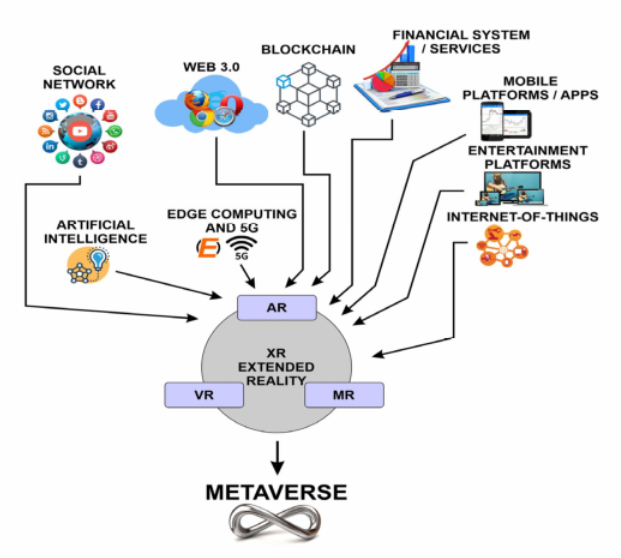
\includegraphics[width=\textwidth]{images/metaverse/metaverseEcosystem.png}
    \caption{Ekosystem Metaverse\cite{metaverseSecurityIssuesChallengesAndViableZTAModel}}
    \label{metaverseEcosystemImage}
\end{figure}

Metaverse umożliwia realizację kilku nowatorskich scenariuszy biznesowych w wielu różnych branżach. Połączenie tych technologii w połączeniu z nowymi rozwiązaniami pomoże zrealizować wizję metawersji w przyszłości. Rysunek \ref{metaverseEcosystemImage} przedstawia nadrzędny ekosystem technologiczny umożliwiający powstanie metawersji. Nie ulega wątpliwości, że technologie AR/VR/MR i XR stanowią podstawę metawersji, umożliwiając użytkownikom dostęp do wirtualnego świata 3D. W swojej najwcześniejszej iteracji metaverse może być zbiorem aplikacji Web 3.0 z XR-Skin zapewniającym ograniczone wrażenia VR. Oczekuje się, że sieci społecznościowe będą jednymi z pierwszych, które przeniosą się do metaverse, umożliwiając użytkownikom udostępnianie i konsumowanie treści immersyjnych wraz z Web 3.0, umożliwiając firmom oferowanie użytkownikom nowatorskich doświadczeń produktowych. Technologia blockchain zostanie szeroko wdrożona w metaverse, aby umożliwić realizację wizji zdecentralizowanych finansów i gospodarki twórców, które są nowymi tematami, głównie ze względu na bezpieczeństwo i prywatność, które oferują. Aplikacje i platformy mobilne mogą być kolejnymi, które migrują do metaverse, a następnie platformy rozrywkowe. Wreszcie, łączność 5G/6G, oferująca niskie opóźnienia, może być spoiwem, które płynnie połączy wszystkie elementy, podczas gdy Internet Rzeczy będzie łączył wszystkie urządzenia wraz z intensywnym wykorzystaniem sztucznej inteligencji, w tym inteligencji brzegowej, w celu zapewnienia spersonalizowanych doświadczeń\cite{metaverseSecurityIssuesChallengesAndViableZTAModel}. 
Można przewidzieć, że ekosystem metaverse przedstawiony na rysunku \ref{metaverseEcosystemImage} może przyjąć trzy potencjalne ścieżki ewolucji:

\begin{itemize}
    \item Zamknięty Metaverse: Dla niszowych aplikacji i przypadków użycia ograniczonych do użytku przez konkretną społeczność o wyspecjalizowanych potrzebach.
    \item Federacyjny: Zarządzana i obsługiwana przez dużą korporację z ekosystemem współpracujących partnerów, zewnętrznych dostawców i usługodawców dostarczających użytkownikom końcowym ujednolicone doświadczenie;  
    \item Otwarty Metaverse: Metawersja niesfederowana, nie kontrolowana przez żaden pojedynczy podmiot. O otwartej architekturze i społeczności deweloperów tworzących aplikacje/usługi dla użytkowników końcowych.
\end{itemize}



Prawdopodobnym jest, że ekosystem metaverse, jak pokazano na rysunku \ref{metaverseEcosystemImage}, może przyjąć trzy formy. Można oczekiwać, że wszystkie trzy modele będą współistnieć w takiej czy innej formie. Meta Facebooka jest doskonałym przykładem metawersji federacyjnej\cite{metaverseSecurityIssuesChallengesAndViableZTAModel}. 

Oczekuje się, że w przyszłości pojawią się inne modele, głównie napędzane przez sojusze biznesowe, fuzje i przejęcia. Jest prawdopodobne, że metaverse napotka kilka przeszkód na drodze do jego szerokiego przyjęcia. Niektóre z wyzwań stojących na drodze do realizacji pełnego potencjału koncepcji metaverse i jej przyjęcia obejmują:

\begin{itemize}
    \item Dostęp: Obecnie tylko przez zestawy okularów wirtualnej rzeczywistości, które nie są aktualnie powszechne
    \item Łatwość użytkowania: Użytkownicy uważają, że obecna wersja zestawów okularów wirtualnej rzeczywistości jest nieporęczna i trudna do noszenia przez długi czas
    \item Brak rozwiniętego ekosystemu: Niewiele aplikacji dostępnych na obecnych platformach VR
    \item Bezpieczeństwo i prywatność: Środowiska XR cierpią z powodu luk w zabezpieczeniach podstawowych technologii, w tym kwestii dotyczących prywatności użytkowników w wirtualnych światach. 
\end{itemize}

Podczas gdy oczekuje się, że postęp technologiczny rozwiąże kwestie dostępu i łatwości użytkowania w najbliższej przyszłości, kwestie bezpieczeństwa i prywatności muszą być budowane od podstaw podczas projektowania ekosystemu metaverse\cite{metaverseSecurityIssuesChallengesAndViableZTAModel}. 


\subsubsection{Podsumowanie}

Metawersja stanowi rewolucyjny skok w sposobie, w jaki ludzie postrzegają środowiska cyfrowe i wchodzą z nimi w interakcję, zacierając granice między sferą fizyczną i wirtualną. U podstaw tej koncepcji leży wiele koncepcji solidnej i zaawansowanej infrastruktury, która posłuży jako podstawa płynnej łączności, wciągających doświadczeń i nieograniczonych możliwości. 

W miarę jak metawersja będzie ewoluować i zyskiwać popularność, jej infrastruktura będzie odgrywać kluczową rolę w kształtowaniu przyszłości cyfrowych interakcji, handlu i kontaktów społecznych. Wykorzystując najnowocześniejsze technologie, takie jak blockchain, rzeczywistość wirtualna, rzeczywistość rozszerzona i zdecentralizowane przetwarzanie, infrastruktura metaverse umożliwia bezpieczne, przejrzyste i interoperacyjne przestrzenie wirtualne.

Pomyślne wdrożenie i rozwój metawersji będzie jednak również wymagać sprostania krytycznym wyzwaniom związanym z zarządzaniem, regulacjami, bezpieczeństwem i prywatnością. Współpraca między zainteresowanymi stronami, w tym deweloperami, decydentami i szerszą społecznością, jest niezbędna do ustanowienia skutecznych ram, które sprzyjają innowacjom, jednocześnie chroniąc użytkowników i utrzymując standardy etyczne.
\chapter{Metaverse --- przegląd literatury}

Niniejszy rozdział przedstawia obecne implementacje Metaverse, podkreślając technologiczne podstawy i wyzwania stojące przed realizacją tego rozwijającego się wirtualnego środowiska. Zaprezentowane informacje oparte są na analizie wybranych artykułów naukowych.

\section{A Survey of Mobile Edge Computing for the
Metaverse: Architectures, Applications, and
Challenges}

Artykuł "A Survey of Mobile Edge Computing for the Metaverse: Architectures, Applications, and Challenges" autorstwa Yitong Wang i Jun Zhao z Nanyang Technological University Singapore bada przede wszystkim możliwość wykorzystania Mobile Edge Computing \akronim{MEC} w środowisku Metaverse, podkreślając aspekty techniczne i infrastrukturę wymaganą do obsługi tak złożonego systemu.

\akronim{MEC} jest definiowany jako rozproszony paradygmat obliczeniowy, który umieszcza zasoby obliczeniowe i pamięć masową na urządzeniach końcowych, w celu realizacji przetwarzania na tych urządzeniach. Zmniejsza to opóźnienia i poprawia wydajność aplikacji poprzez przeniesienie intensywnych zadań na pobliskie serwery brzegowe.

\subsection{Infrastruktura sieciowa}

Wdrożenie sieci \akronim{5G} ma kluczowe znaczenie dla Metaverse ze względu na wysoką szybkość transmisji danych, niskie opóźnienia i wysoką gęstość połączeń. Integracja \akronim{MEC} z sieciami \akronim{5G} zapewnia, że dane generowane przez urządzenia, takie jak zestawy VR, mogą być przetwarzane szybko i wydajnie.

Serwery zlokalizowane na brzegu sieci, wykonują zadania obliczeniowe odciążające urządzenia końcowe, zmniejszając w ten sposób obciążenie sieci rdzeniowych i zapewniając przetwarzanie w czasie rzeczywistym.

\subsection{Paradygmaty obliczeniowe}

Podczas gdy tradycyjne przetwarzanie w chmurze aktualnie odgrywa kluczową rolę w systemach rozproszonych, poleganie wyłącznie na serwerach w chmurze może powodować duże opóźnienia i przeciążenia sieci. Dlatego konieczne jest podejście hybrydowe obejmujące przetwarzanie brzegowe i przetwarzanie we mgle (\english{fog computing}).

Przetwarzanie we mgle działa jako warstwa pośrednia między chmurą a urządzeniami brzegowymi, obsługując zadania, które wymagają mniejszych opóźnień niż może zaoferować chmura, ale są zbyt intensywne dla samych urządzeń brzegowych.

\subsection{Transmisja i przetwarzanie danych}

Przetwarzając dane bliżej źródła ich generowania (np. na serwerach brzegowych), MEC znacznie zmniejsza opóźnienia w porównaniu z tradycyjnymi rozwiązaniami opartymi na chmurze. Ma to kluczowe znaczenie dla immersyjnych doświadczeń w czasie rzeczywistym wymaganych w Metaverse.

\akronim{MEC} pomaga w zarządzaniu wykładniczym wzrostem ruchu danych poprzez przetwarzanie i filtrowanie danych na krawędzi przed przesłaniem ich do chmury, optymalizując w ten sposób wykorzystanie przepustowości

\subsection{Modele architektury}

Architektura Metaverse oparta na \akronim{MEC}, zaprezentowana na rys.\ref{mecBaseArch} obejmuje dynamiczne węzły brzegowe do obsługi interakcji użytkownika i przetwarzania danych, minimalizując w ten sposób opóźnienia i poprawiając doświadczenia świadczonych usług przez użytkownika.

\begin{figure}[htbp!]
    \centering
    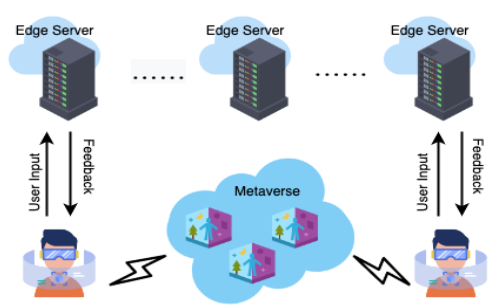
\includegraphics[width=0.85\textwidth]{images/existingArchitectres/mecBaseArch.png}
    \caption{Architektura Metaverse wykorzystująca Mobile Edge Computing}
    \label{mecBaseArch}
\end{figure}

\newpage
Architektura oparta na przetwarzaniu we mgle proponuje wielopoziomowe podejście, w którym różne zadania obliczeniowe są dystrybuowane w warstwach mgły, krawędzi i chmury w celu optymalizacji wydajności i zmniejszenia wąskich gardeł obliczeniowych.

Artykuł podkreśla znaczenie \akronim{MEC} w infrastrukturze Metaverse poprzez rozwiązywanie krytycznych kwestii, takich jak opóźnienia, wydajność przepustowości i zarządzanie zasobami obliczeniowymi. Przybliżając moc obliczeniową do użytkowników końcowych i wykorzystując zaawansowaną infrastrukturę sieciową, taką jak \akronim{5G}, paradygmat \akronim{MEC} jest niezbędny do implementacji świata Metaverse.

\section{Dynamic Resource Allocation for Metaverse Applications with Deep Reinforcement Learning}

Artykuł "Dynamic Resource Allocation for Metaverse Applications with Deep Reinforcement Learning" autorstwa Nam H. Chu,
Eryk Dutkiewicz, Diep N. Nguyen, Dinh Thai Hoang, Khoa T. Phan, Dusit Niyato i Tao Shu koncentruje się na infrastrukturze i aspektach technicznych wymaganych do efektywnego zarządzania ogromnym zapotrzebowaniem na zasoby aplikacji Metaverse.

\subsection{Wyzwania związane z zarządzaniem zasobami}

Autorzy w artykule wskazują następujące wyzwania związane z zarządzaniem zasobami w środowisku Metaverse:

\begin{itemize}
    \item Aplikacje Metaverse wymagają dużych zasobów obliczeniowych, pamięci masowej i sieci, które przekraczają możliwości istniejących systemów.
    \item Dynamiczny i niepewny charakter żądań użytkowników i cykli życia aplikacji wymaga zaawansowanych strategii zarządzania zasobami.
\end{itemize}

\subsection{Proponowane rozwiązania}

Autorzy proponują następujące rozwiązania:
\begin{itemize}
    \item MetaInstancje i MetaSlices --- Aplikacje są podzielone na MetaInstancje, w których funkcje mogą być współdzielone między aplikacjami w celu zwiększenia efektywności wykorzystania zasobów.
    \item Architektura wielowarstwowa --- Framework wykorzystuje wielowarstwową architekturę chmury obliczeniowej do efektywnej dystrybucji zasobów z chmury do brzegu sieci, zmniejszając opóźnienia i przeciążenia.
\end{itemize}

\subsection{Wielowarstwowa architektura obliczeniowa}

Warstwowa dystrybucja zasobów zaprezentowana na rys.\ref{metaslicingMultiTierArch} zapewnia, że zasoby są dystrybuowane na wielu poziomach, od użytkowników końcowych po serwery w chmurze, aby zrównoważyć obciążenie i zoptymalizować wydajność.

\begin{figure}[!htbp]
    \centering
    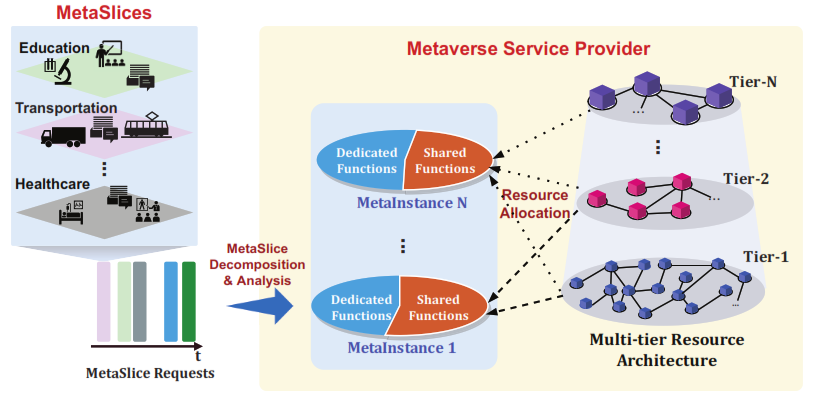
\includegraphics[width=\textwidth]{images/existingArchitectres/dynamicResourcemetaslicingMultiTierArch.png}
    \caption{Warstwowa dystrybucja zasobów}
    \label{metaslicingMultiTierArch}
\end{figure}

Dekompozycja aplikacji powoduje że aplikacje są dzielone na mniejsze funkcje, z których każda jest wykonywana na różnych poziomach w oparciu o ich wymagania dotyczące zasobów i dostępne możliwości.

Artykuł przedstawia zaawansowany framework do dynamicznego zarządzania i alokacji zasobów w Metaverse przy użyciu kombinacji wielowarstwowego przetwarzania w chmurze i zaawansowanych technik głębokiego uczenia ze wzmocnieniem. Dzięki dekompozycji aplikacji na MetaSlices i MetaInstances oraz zastosowaniu procesu decyzyjnego semi-Markova, framework skutecznie radzi sobie z ogromnym i dynamicznym zapotrzebowaniem na zasoby aplikacji Metaverse.

\section{Unlocking Metaverse-as-a-Service}

Artykuł "Unlocking Metaverse-as-a-Service" autorstwa Vesal Ahsani, Ali Rahimi, 
Mehdi Letafati, Babak Hossein Khalaj, omawia niezbędną infrastrukturę techniczną i wyzwania związane z wdrażaniem platform Metaverse-as-a-Service \akronim{MaaS}.

\subsection{Główne filary MaaS}

Autorzy wskazują trzy główne filary:
\begin{itemize}
    \item Prywatność i bezpieczeństwo --- Zapewnienie bezpiecznych i prywatnych interakcji w Metaverse jest najważniejsze. Artykuł kładzie nacisk na mechanizmy prywatyzacji wrażliwych atrybutów danych i zabezpieczania rozproszonych algorytmów uczenia maszynowego.
    \item Przetwarzanie brzegowe --- wzmacnia Metaverse poprzez zmniejszenie opóźnień i przeciążenia sieci. Obejmuje przetwarzanie i przechowywanie danych blisko użytkowników końcowych, zwiększając wydajność i skalowalność aplikacji Metaverse
    \item Technologia Blockchain --- Blockchain zapewnia przejrzystość, integralność danych i bezpieczne transakcje w ramach Metaverse. Obsługuje zdecentralizowane aplikacje i inteligentne kontrakty, niezbędne dla ekonomicznej i operacyjnej integralności Metaverse.
\end{itemize}

\subsection{Przetwarzanie brzegowe w Maas}

Struktura \akronim{MaaS} opiera się w dużej mierze na przetwarzaniu brzegowym, w którym przetwarzanie i przechowywanie danych odbywa się blisko użytkowników, zmniejszając opóźnienia i poprawiając wrażenia użytkownika. Serwery brzegowe mają kluczowe znaczenie dla obsługi lokalnego przetwarzania danych, pamięci masowej i funkcji sieciowych. Odciążają intensywne zadania z centralnych serwerów w chmurze, optymalizując ruch sieciowy i zwiększając możliwości przetwarzania danych w czasie rzeczywistym.

\subsection{Infrastruktura sieciowa}

Sieci 5G/6G --- Szybkie sieci bezprzewodowe o niskich opóźnieniach są niezbędne do obsługi wymagań Metaverse w czasie rzeczywistym. Sieci te ułatwiają płynny transfer danych między urządzeniami brzegowymi a serwerami. 

Bramy internetowe --- Łączą one systemy brzegowe z szerszą infrastrukturą sieciową i chmurową, zapewniając wydajny przepływ danych.

\subsection{Zarządzanie danymi i bezpieczeństwo}

Kontrola danych --- Przetwarzanie brzegowe zwiększa kontrolę nad danymi, utrzymując je blisko źródła, zapewniając lepsze zarządzanie prywatnością i bezpieczeństwem. Ma to kluczowe znaczenie dla obsługi danych wrażliwych, takich jak dane biometryczne i informacje zdrowotne.
Bezpieczna wymiana danych: Technologia Blockchain zapewnia, że dane udostępniane w ramach Metaverse są bezpieczne i niezmienne. Technologia ta wspiera bezpieczne transakcje i interakcje między użytkownikami i aplikacjami.

\subsection{Optymalizacja wydajności}

Przetwarzając dane na brzegu sieci, platforma znacząco redukuje opóźnienia, co ma kluczowe znaczenie dla aplikacji działających w czasie rzeczywistym, takich jak AR/VR i interaktywne gry.
Przetwarzanie brzegowe optymalizuje przepustowość sieci poprzez lokalne przetwarzanie danych, zmniejszając potrzebę przesyłania dużych ilości danych do centralnych serwerów.

Artykuł przedstawia infrastrukturę techniczną wymaganą do obsługi platform Metaverse-as-a-Service, koncentrując się na prywatności i bezpieczeństwie, przetwarzaniu brzegowym i technologii blockchain. Przetwarzanie brzegowe odgrywa kluczową rolę w zmniejszaniu opóźnień i optymalizacji wydajności sieci, podczas gdy blockchain zapewnia integralność danych i bezpieczne transakcje. Integracja tych technologii tworzy solidne, skalowalne i bezpieczne ramy dla Metaverse, zdolne do obsługi rozległych i dynamicznych wymagań dotyczących zasobów w immersyjnych środowiskach wirtualnych.


\section{Porównanie i podsumowanie}

Wszystkie trzy artykuły podkreślają kluczową rolę zaawansowanych technologii i infrastruktury we wdrażaniu środowiska Metaverse. W szczególności omówione prace analizują komponenty niezbędne dla działania tego środowiska i wyzwania stawiane przed jego twórcami. Poddane analizie prace skupiają się w szczególności na następujących aspektach: 
\begin{itemize}
    \item Koncentracja na zaawansowanych technologiach:
    \begin{itemize}
        \item Wszystkie artykuły podkreślają znaczenie zaawansowanych technologii, takich jak przetwarzanie brzegowe i sieci \akronim{5G/6G} we wdrażaniu aplikacji Metaverse.
        \item Podkreślają potrzebę skalowalnego, wydajnego zarządzania zasobami w celu obsługi wysokich wymagań aplikacji Metaverse.
    \end{itemize}
    \item Wymagania dotyczące infrastruktury:
    \begin{itemize}
        \item Artykuły omawiają krytyczne komponenty infrastruktury niezbędne dla Metaverse, w tym serwery brzegowe, przetwarzanie w chmurze i architekturę sieci.
        \item Wszystkie artykuły podkreślają rolę przetwarzania brzegowego w zmniejszaniu opóźnień i poprawie wydajności poprzez przetwarzanie danych bliżej źródła.
    \end{itemize}
    \item Wyzwania związane z wdrażaniem Metaverse:
    \begin{itemize}
        \item Wszystkie artykuły dostrzegają wyzwania związane z wdrażaniem aplikacji Metaverse, takie jak opóźnienia, wydajność przepustowości i potrzeba przetwarzania w czasie rzeczywistym.
        \item Uznają one trudności w zarządzaniu ogromnymi danymi i wymaganiami obliczeniowymi aplikacji Metaverse.
    \end{itemize}
\end{itemize}

Chociaż artykuły mają wspólną płaszczyznę, koncentrując się na technologicznych podstawach Metaverse, różnią się one w swoich konkretnych podejściach, ramach i obszarach nacisku. Kluczowe różnice między tymi badaniami to:
\begin{itemize}
    \item Konkretne obszary tematyczne:
    \begin{itemize}
        \item "A Survey of Mobile Edge Computing for the Metaverse: Architectures, Applications, and Challenges": Ten artykuł koncentruje się na integracji Mobile Edge Computing z Metaverse, szczegółowo opisując architektury, aplikacje i wyzwania związane z tą integracją.
        \item "Dynamic Resource Allocation for Metaverse Applications with Deep Reinforcement Learning": Ten artykuł koncentruje się na dynamicznej alokacji zasobów przy użyciu technik głębokiego uczenia się ze wzmocnieniem, zapewniając szczegółowe frameworki i inteligentny algorytm optymalizacji zarządzania zasobami w Metaverse.
        \item "Unlocking Metaverse-as-a-Service": Ten artykuł podkreśla koncepcję Metaverse-as-a-Service, koncentrując się na prywatności i bezpieczeństwie, przetwarzaniu brzegowym i technologii blockchain jako głównych filarach wspierających infrastrukturę MaaS.
    \end{itemize}
    \item Podejście do zarządzania zasobami:
    \begin{itemize}
        \item  Pierwszy artykuł podkreśla rolę MEC w ulepszaniu aplikacji Metaverse poprzez zmniejszenie opóźnień i poprawę wydajności przetwarzania danych poprzez przetwarzanie brzegowe.
        Drugi artykuł koncentruje się na wykorzystaniu głębokiego uczenia ze wzmocnieniem do dynamicznego przydzielania zasobów, prezentując podejście algorytmiczne do zarządzania wysokim i zmiennym zapotrzebowaniem na zasoby aplikacji Metaverse.
        W artykule MaaS omówiono, w jaki sposób MaaS może być wykorzystywany do świadczenia skalowalnych usług na żądanie, podkreślając integrację przetwarzania brzegowego i łańcucha bloków w celu zapewnienia bezpiecznych, wydajnych i skalowalnych usług Metaverse.
    \end{itemize}
    \item Szczegóły infrastruktury sieciowej:
    \begin{itemize}
        \item Artykuł MEC zagłębia się w specyfikę architektur sieciowych niezbędnych do integracji MEC z sieciami \akronim{5G}, podkreślając, w jaki sposób serwery brzegowe mogą odciążać zadania z urządzeń końcowych.
        \item Artykuł dotyczący dynamicznej alokacji zasobów proponuje wielowarstwową architekturę chmury obliczeniowej w celu efektywnej dystrybucji zasobów, eliminacji wąskich gardeł obliczeniowych i optymalizacji wydajności poprzez podejście warstwowe.
        \item Artykuł MaaS omawia, w jaki sposób technologia blockchain może zostać zintegrowana z infrastrukturą Metaverse w celu zwiększenia bezpieczeństwa, przejrzystości i integralności danych, uzupełniając podejście Edge Computing w celu zmniejszenia opóźnień i poprawy świadczenia usług.
    \end{itemize}
    \item Transmisja i przetwarzanie danych:
    \begin{itemize}
        \item W artykule poświęconym MEC omówiono korzyści płynące z przetwarzania danych na brzegu sieci w celu zmniejszenia opóźnień i bardziej efektywnego zarządzania ruchem danych.
        \item Drugi artykuł kładzie nacisk na zarządzanie zasobami w czasie rzeczywistym przy użyciu zaawansowanych algorytmów w celu zapewnienia optymalnej wydajności i jakości usług w Metaverse.
        \item Artykuł MaaS podkreśla znaczenie bezpiecznej obsługi danych i prywatności, wykorzystując blockchain w celu zapewnienia integralności danych i przetwarzania brzegowego w celu wydajnego przetwarzania w czasie rzeczywistym.
    \end{itemize}
\end{itemize}

Wszystkie trzy artykuły wnoszą cenny wkład w infrastrukturę techniczną i strategie zarządzania zasobami niezbędne do wdrożenia Metaverse. Są one podobne pod względem skupienia się na zaawansowanych technologiach i wyzwaniach, ale różnią się konkretnymi podejściami i szczegółowymi frameworkami. Artykuł koncentrujący się na MEC zapewnia szerszy przegląd architektur sieciowych i przetwarzania brzegowego, artykuł o alokacji zasobów oferuje głębokie zanurzenie w algorytmicznych rozwiązaniach do zarządzania zasobami w czasie rzeczywistym, a artykuł MaaS kładzie nacisk na integrację przetwarzania brzegowego i blockchain w celu stworzenia skalowalnej i bezpiecznej platformy Metaverse-as-a-Service.
\chapter{Koncepcja i architektura systemu}

Niniejszy rozdział opisuje architekturę i koncepcję systemu zaprojektowanego do obsługi środowiska Metaverse. Poprzez integrację różnych technologii. System ten ułatwia dynamiczne wykrywanie usług, solidne przetwarzanie danych i monitorowanie w czasie rzeczywistym. Celem jest stworzenie skalowalnego i interaktywnego wirtualnego świata, w którym producenci i użytkownicy mogą płynnie wchodzić w interakcje, zapewniając optymalną wydajność i niezawodność dzięki skutecznym praktykom monitorowania systemu.

System przedstawiony na rys.\ref{designedSystem} został zaprojektowany w celu wspierania dynamicznego i interaktywnego środowiska Metaverse poprzez integrację dwóch podstawowych podsystemów: jednego skoncentrowanego na producentach i użytkownikach, a drugiego na monitorowaniu i utrzymaniu.

% Temporarily change the margins for this page
\newgeometry{
  left=0.5in,
  right=0.5in,
  top=1.5in,
  bottom=1in,
}
\begin{figure}[!htbp]
    \centering
    \includesvg[width=\textwidth]{schemas/master—koncepcja-Dev.drawio.svg}
    \caption{Schemat tworzonego systemu}
    \label{designedSystem}
\end{figure}
% Restore the original margins
\restoregeometry
\newpage


\section{Podsystem użytkowy}

Podsystem użytkowy ułatwia interakcję między producentami i użytkownikami. Producenci to podmioty, które tworzą i dostarczają wirtualne środowiska, zasoby cyfrowe lub usługi w ramach Metaverse. Z kolei użytkownicy wykorzystują te zasoby, aby uczestniczyć w różnych działaniach i doświadczeniach. Każdy użytkownik uruchamia wyspecjalizowaną aplikację z unikalnym identyfikatorem, co pozwala mu na interakcję z systemem, żądanie zasobów i płynną współpracę z producentami. Rejestr usług zapewnia, że producenci i użytkownicy mogą dynamicznie odkrywać i wchodzić ze sobą w interakcje, wspierając wydajny i skalowalny ekosystem.

\subsection{Rejestr usług}

Pierwszym centralnym elementem podsystemu użytkowego jest rejestr usług, który zarządza wykrywaniem i przechowywaniem informacji o uruchomionych usługach w sieci. Komponent ten działa jako centralny katalog, w którym każda usługa rejestruje się po uruchomieniu, podając szczegóły, takie jak jej lokalizacja i status. Inne usługi i aplikacje w sieci mogą następnie odpytywać ten rejestr, aby znaleźć i uzyskać informacje o zarejestrowanych usługach. Mechanizm ten zapewnia, że wszystkie usługi mogą dynamicznie lokalizować się nawzajem i efektywnie współdziałać, wspierając płynną komunikację i alokację zasobów w systemie.

\subsection{Producenci}

W zaprojektowanym systemie producenci są podmiotami, które tworzą i oferują różne wirtualne produkty i usługi. Producenci muszą najpierw zarejestrować się w centralnym rejestrze usług. Po zarejestrowaniu producenci stają się wykrywalni przez inne komponenty i użytkowników w systemie. Po rejestracji producenci są odpowiedzialni za dostarczanie swoich produktów i usług, oraz na żądanie użytkownika zapewniają, że ich oferty są dostępne dla użytkowników. Ten proces rejestracji i wykrywania ułatwia wydajną interakcję i wykorzystanie zasobów w środowisku Metaverse.

\subsection{Użytkownicy}

Aby uczestniczyć w przetwarzaniu systemu i zamawiać zasoby od producentów, użytkownicy muszą uruchomić usługę węzła protokołu z unikalnym identyfikatorem. Ten unikalny identyfikator jest niezbędny do identyfikacji i zarządzania interakcjami każdego użytkownika w systemie.

\subsubsection{Funkcje i działania użytkownika}

Zaprojektowany użytkownik zapewnia następujące funkcje:

\begin{itemize}
    \item Aplikacja węzła protokołu: Użytkownicy są zobowiązani do uruchomienia usługi o nazwie protocol-worker. Aplikacja ta służy jako interfejs, za pośrednictwem którego użytkownicy wchodzą w interakcję z systemem Metaverse, umożliwiając im żądanie zasobów dostarczanych przez producentów.
    \item W momencie uruchomienia usługi zostaje jej nadany unikatowy w skali systemu identyfikator. Ten identyfikator ma kluczowe znaczenie dla śledzenia działań użytkownika, zarządzania jego żądaniami i zapewnienia, że zasoby są odpowiednio przydzielane.
    \item Rejestracja usługi w serwerze usług: Aplikacja protocol-worker rejestruje się w serwerze usług przy użyciu unikalnego identyfikatora. Ten proces rejestracji sprawia, że użytkownik jest wykrywalny w systemie Metaverse.
    \item Zamawianie zasobów: Po rejestracji użytkownicy mogą zamawiać zasoby od producentów w systemie. Aplikacja protocol-worker zapewnia te interakcje, zbierając dane monitorujące producentów w celu późniejszego określenia, który z nich jest najbardziej odpowiedni dla użytkownika zamawiającego zasoby.
\end{itemize}

Na rys.\ref{wymianaWiadomosciWSystemie} przedstawiono sekwencję wymiany komunikatów w ramach systemu rezerwacji zasobów. Wykres ten szczegółowo opisuje interakcje pomiędzy elementami systemu:

\begin{itemize}
    \item Proces rozpoczyna się od zainicjowania przez użytkownika żądania rezerwacji zasobów. Żądanie to jest wysyłane do usługi  protocol-worker.
    \item Po otrzymaniu żądania użytkownika, usługa protocol-worker wysyła zapytanie do rejestru usług w celu uzyskania listy wszystkich zarejestrowanych producentów. Ten krok zapewnia, że protocol-worker ma najbardziej aktualne informacje o dostępnych producentach w systemie.
    \item Rejestr usług odpowiada na żądanie usługi protocol-worker z listą zarejestrowanych producentów. Lista ta zawiera informacje o producentach, którzy mogą potencjalnie spełnić żądanie użytkownika.
    \item Usługa protocol-worker przetwarza każdego producenta z listy, aby sprawdzić dostępność żądanych zasobów.
    \item Dla każdego producenta na liście usługa protocol-worker wysyła wiadomości w celu sprawdzenia dostępności żądanych zasobów. Wiąże się to z wysłaniem zapytania do producenta w celu ustalenia, czy może on zapewnić wymagane zasoby.
    \item Każdy producent odpowiada do protocol-worker z informacją o dostępności żądanych zasobów. Ta odpowiedź wskazuje, czy producent może spełnić żądanie użytkownika.
    \item Po zebraniu informacji o dostępności zasobów od wszystkich producentów, usługa protocol-worker przetwarza te odpowiedzi w celu określenia najlepszych opcji realizacji żądania użytkownika. Może to obejmować wybór producentów, którzy mogą najbardziej efektywnie zapewnić niezbędne zasoby.
    \item Na koniec usługa protocol-worker zwraca użytkownikowi zebrane informacje o dostępności zasobów u producentów.
\end{itemize}

\begin{figure}[h!]
    \centering
    \begin{msc}[
        title position=center,
        msc keyword=,
        draw frame=none,
        instance distance=2.5cm,
        left environment distance=0.5cm,
        right environment distance=0.5cm,
        label distance=0.3cm,
        title distance=0.5cm
        ]{Protocol Worker Resource Reservation}
            \declinst{user}{}{User}
            \declinst{protocolWorker}{}{Protocol Worker}
            \declinst{serviceDiscovery}{}{Service Discovery}
            \declinst{producer}{}{Producer}
            
            \footnotesize
            \nextlevel
            \mess{Request Resource Reservation}{user}{protocolWorker}
            \nextlevel
            \nextlevel
            \mess{Query All Registered Producers}{protocolWorker}{serviceDiscovery}
            \nextlevel
            \nextlevel
            \nextlevel
            \mess{List of Producers}{serviceDiscovery}{protocolWorker}
            \nextlevel
            \nextlevel
            \nextlevel
            \inlinestart{loop1}{loop for each Producer}{protocolWorker}{producer}
            \nextlevel
            \nextlevel
            \nextlevel
            \nextlevel
            \mess{Check Resource Availability}{protocolWorker}{producer}
            \nextlevel
            \nextlevel
            \nextlevel
            \mess{Resource Availability}{producer}{protocolWorker}
            \nextlevel
            \nextlevel
            \inlineend{loop1}
            \nextlevel
            \nextlevel
            \mess{\parbox{3cm}{Processing producers for products}}{protocolWorker}{protocolWorker}
            \nextlevel
            \nextlevel
            \nextlevel
            \nextlevel
            \nextlevel
            \mess{Return Resource Availability}{protocolWorker}{user}
        \end{msc}
    \caption{ Schemat wymiany wiadomości podczas przetwarzania żądania użytkownika}
    \label{wymianaWiadomosciWSystemie}
\end{figure}

\section{Podsystem monitoringu}

Drugi podsystem jest przeznaczony do monitorowania i utrzymywania kondycji i wydajności infrastruktury Metaverse. Podsystem ten stale gromadzi i przetwarza dzienniki zdarzeń ze wszystkich komponentów systemu, zapewniając wgląd w czasie rzeczywistym w działania systemu. Dzięki kompleksowym narzędziom wizualizacyjnym administratorzy mogą monitorować stan systemu, identyfikować potencjalne problemy i podejmować decyzje oparte na danych w celu zapewnienia optymalnej funkcjonalności. Takie podejście do monitorowania i konserwacji pomaga utrzymać niezawodne i wydajne środowisko Metaverse, wspierając płynną interakcję między producentami i użytkownikami.
\chapter{Wybrane narzędzia i technologie}


W pracy magisterskiej podczas opracowywania i wdrażania systemu wykorzystano rozmaite narzędzia i technologie. Każde narzędzie odgrywa kluczową rolę w zapewnieniu wydajności, skalowalności i łatwości utrzymania systemu.

\section{Java}

\begin{figure}[!htbp]
    \centering
    
\includegraphics[width=0.1\textwidth]{images/javaLogo.png}
    \caption{Oficjalne logo języka Java}
    \label{fig:enter-label}
\end{figure}

Java jest to szeroko stosowany obiektowy język programowania i platforma oprogramowania, która działa na miliardach urządzeń. Zasady oraz składnia języka zostały oparte na językach \acronym{C} i \acronym{C++}\cite{javaIBM}\cite{cstandard}\cite{cppstandard}. Java powstała aby udoskonalić i naprawić wiele błędnych konceptów wprowadzonych przez te języki. Jedną z głównych zalet tworzenia oprogramowania w Javie jest jej przenoszalność. Po napisaniu kodu programu na jednym urządzeniu można go łatwo przenieść na inne urządzenie o innej architekturze. Język ten został wynaleziony w 1995 roku przez Jamesa Goslinga z Sun Microsystems (później przejętego przez Oracle), główną ideą jego wynalezienia była możliwość, \definicja{"napisania raz, uruchomienia w dowolnym miejscu"}  (\english{write once, run anywhere}). Nowe i ulepszone narzędzia do tworzenia oprogramowania pojawiają się na rynku w niezwykłym tempie, wypierając dotychczasowe produkty, które kiedyś uważano za niezbędne. W świetle tej ciągłej rotacji, trwałość i ciągła popularność języka Java jest imponująca, prawie trzy dekady po jej stworzeniu, Java jest nadal jednym z najbardziej popularnych języków do tworzenia oprogramowania użytkowego\cite{javaIBM}\cite{javaDEV}.

Wszystkie języki programowania służą do komunikacji z maszynami. Sprzęt maszynowy reaguje tylko na komunikację elektroniczną. Języki programowania wysokiego poziomu, takie jak Java, działają jako pomost między językiem ludzkim a językiem sprzętu. Aby korzystać z języka Java, programista powinien mieć świadomość istnienia dwóch poziomów abstrakcji pisanych programów: 

\begin{itemize}
    \item Język Java i \definicja{interfejsy \acronym{API} }(\english{application programming interface})
    \item Wirtualna maszyna Java \acronym{JVM} (\english{\termdef{Java Virtual Machine}})
\end{itemize}

Java definiuje składnię i semantykę języka. Obejmuje to podstawowe słownictwo i reguły używane do pisania algorytmów. 
Interfejsy API są ważnymi komponentami oprogramowania dołączonymi do platformy Java. Są to wstępnie napisane programy, które można podłączyć i odtworzyć istniejące funkcjonalności we własnym kodzie. Na przykład można użyć interfejsów API Java, aby uzyskać datę i godzinę, wykonać operacje matematyczne lub manipulować tekstem. Każdy kod aplikacji Java napisany przez programistę zazwyczaj łączy nowy i wcześniej istniejący kod z interfejsów API Java, bibliotek i frameworków\cite{frameworkDef}\cite{javaAmazon}\cite{javaDEV}.

Wirtualna maszyna Javy działa jako dodatkowa warstwa abstrakcji między platformą Java a sprzętem maszyny. Kod źródłowy Java może działać tylko na tych maszynach na których zainstalowano JVM. Kiedy po raz pierwszy opracowano języki programowania, dzieliły się one na dwie szerokie kategorie, w zależności od tego, w jaki sposób komunikowały się ze sprzętem: 

\begin{itemize}
    \item \textbf{Kompilowany} --- program jest napisany w składni języka, a następnie kompilator tłumaczy cały kod na kod maszynowy. Skompilowany kod jest następnie uruchamiany na sprzęcie.
    \item \textbf{Interpretowany} --- Dzięki interpreterom każda instrukcja kodu wysokiego poziomu jest na bieżąco interpretowana na kod maszynowy. Napisane instrukcje są natychmiast uruchamiane przez sprzęt przed przejściem do następnej instrukcji
\end{itemize}

Język Java był pierwszym językiem, który połączył obie powyższe metody, przy użyciu JVM. Każdy plik programu jest najpierw kompilowany do kodu bajtowego (\english{bytecode}). Kod bajtowy Java może być uruchamiany tylko w maszynie JVM. Następnie JVM interpretuje kod bajtowy, aby uruchomić go na podstawowej platformie sprzętowej. Jeżeli aplikacja działa na komputerze z systemem Windows, maszyna JVM zinterpretuje ją dla systemu Windows. Natomiast jeżeli aplikacja uruchomiona jest na platformie open--source, takiej jak Linux, JVM zinterpretuje ją dla systemu Linux\cite{javaAmazon}\cite{javaDEV}.

\section{Maven}

\begin{figure}[htbp!]
    \centering
    
\includegraphics[width=0.2\textwidth]{images/mavenLogo.png}
    \caption{Logo programu Apache Maven\cite{mavenSite}.}
    \label{fig:enter-label}
\end{figure}

Słowo maven  w języku jidysz oznacza gromadzenie wiedzy. Apache Maven to narzędzie do zarządzania projektami oprogramowania. Opiera się ono na koncepcji \definicja{modelu obiektu projektu} (\acronym{POM} \english{Project Object Model}), Maven może zarządzać kompilacją, raportowaniem i dokumentacją projektu na podstawie centralnej informacji. Narzędzie to wykorzystywane jest do budowania i zarządzania dowolnym projektem opartym na języku Java. Głównym źródłem informacji o projekcie jest plik \akronim{XML} (\english{Extensible Markup Language}) nazywany \acronym{POM}, w którym definiowana jest struktura projektu, sposób jego budowania oraz zależności jakie są wymagane do prawidłowego funkcjonowania programu. Maven podcza budowania aplikacji pobiera niezbędne biblioteki oraz inne zależności z globalnego repozytorium Maven Central\cite{mavenSite}.

\section{Spring boot}

\begin{figure}[!htbp]
    \centering
    
\includegraphics[width=0.2\textwidth]{images/springboot/springBootLogo.png}
    \caption{Logo frameworka Spring Boot \cite{springLogo}}
    \label{fig:enter-label}
\end{figure}


Spring boot jest jednym z najpopularniejszych frameworków języka Java zaproponowanym przez Roda Johnsona w 2014 roku, który zapewnia funkcjonalność szybkiego wytwarzania aplikacji (\english{\definicja{Rapid Application Development \akronim{RAD}}}) polegającego na udostępnianiu programiście dużych możliwości prototypowania oraz dużego zestawu gotowych komponentów, narzędzi i modułów\cite{RADwiki}. Spring boot zbudowany jest na popularnym Java Spring Framework, aby zapewnić szybki dostęp do informacji podczas tworzenia projektu. Metodyka RAD jest dość łatwa do skonfigurowania i uruchomienia w internetowych i korporacyjnych aplikacjach przy użyciu języka Java. Najważniejszą rzeczą w tym frameworku jest jego prostota, do uruchomienia aplikacji wymagana jest minimalna konfiguracja, dzięki czemu tworzenie samodzielnych aplikacji opartych na Springu jest o wiele łatwiejsze\cite{springbootAnalysis}.

\subsubsection{Główne cechy Spring Boot Framework}

\begin{enumerate}
    \item \textbf{Autokonfiguracja}: Funkcja automatycznej konfiguracji Spring Boot automatycznie konfiguruje aplikację Spring na podstawie dodanych zależności. Na przykład, jeżeli została dołączona zależność spring--boot--starter--web, automatycznie zostaje skonfigurowany serwer Tomcat i Spring \acronym{MVC} (\english{Model--View--Controller})\cite{springbootFeatures}.
    \item \textbf{Samodzielna aplikacja}: Aplikacje Spring Boot mogą być uruchamiane jako samodzielne aplikacje Java. Jest to ułatwione dzięki osadzeniu serwera HTTP (takiego jak Tomcat, Jetty lub Undertow) bezpośrednio w aplikacji, co ułatwia jej wdrożenie\cite{springbootFeatures}.
    \item \textbf{Funkcje gotowe do produkcji}: Spring Boot zawiera kilka wbudowanych funkcji ułatwiających uruchamianie aplikacji w środowisku produkcyjnym. Obejmują one kontrole kondycji, metryki, monitorowanie aplikacji i konfigurację zewnętrzną\cite{springbootFeatures}.
    \item \textbf{Konwencja ponad konfiguracją}: Spring Boot kieruje się filozofią zapewniania wartości domyślnych, aby zminimalizować ilość wymaganej konfiguracji. Jednak nadal pozwala na zastąpienie tych domyślnych ustawień, gdy jest to konieczne\cite{springbootFeatures}.
    \item \textbf{Rozwój mikrousług}: Spring Boot jest szeroko stosowany do tworzenia mikrousług ze względu na jego lekki i modułowy charakter. Zapewnia wbudowane serwery, łatwą integrację ze środowiskami chmurowymi i wsparcie dla systemów rozproszonych\cite{springbootFeatures}.
    \item \textbf{Startery Spring Boot}: Startery to zestaw wygodnych deskryptorów zależności, które można dołączyć do aplikacji. Na przykład spring-boot--starter--data--jpa zawiera zależności do używania \acronym{JPA} (\english{Java Persistence \acronym{API}}) ze Spring Data\cite{springbootFeatures}.
    \item \textbf{Wbudowane serwery}: Spring Boot obsługuje wbudowane serwery, takie jak Tomcat, Jetty i Undertow, umożliwiając pakowanie aplikacji jako plików \acronym{JAR} (\english{Java Archive}) i uruchamianie ich niezależnie od zewnętrznych serwerów\cite{springbootFeatures}.
    \item \textbf{Spring Initializr}: Spring Initializr to narzędzie internetowe do szybkiego generowania struktury projektu Spring Boot. Pozwala programistom wybrać żądane zależności projektu i wygenerować szkielet projektu\cite{springbootFeatures}.
    \item \textbf{Obszerna dokumentacja i wsparcie społeczności}: Spring Boot jest dobrze udokumentowany i ma dużą i aktywną społeczność, która przyczynia się do jego ciągłego rozwoju i wsparcia\cite{springbootFeatures}.
    \item Korzystając ze Spring Boot, programiści mogą usprawnić tworzenie aplikacji opartych na Spring, wykorzystując potężne funkcje frameworka w celu zmniejszenia ilości standardowego kodu i wysiłku związanego z konfiguracją\cite{springbootFeatures}.
\end{enumerate}

\begin{lstlisting}[caption=Przykładowy podstawowy program , label=basicSpringBootClass]
    package com.example.demo;
    
    import org.springframework.boot.SpringApplication;
    import org.springframework.boot.autoconfigure.SpringBootApplication;
    import org.springframework.web.bind.annotation.GetMapping;
    import org.springframework.web.bind.annotation.RequestParam;
    import org.springframework.web.bind.annotation.RestController;
    
    @SpringBootApplication
    @RestController
    public class DemoApplication {
        public static void main(String[] args) {
          SpringApplication.run(DemoApplication.class, args);
        }
        @GetMapping("/hello")
        public String hello(@RequestParam(value = "name", defaultValue = "World") String name) {
          return String.format("Hello %s!", name);
        }
    }
\end{lstlisting}

Powyższy program składa się z głównej klasy aplikacji z adnotacją @SpringBootApplication, która wskazuje klasę konfiguracyjną, która deklaruje jedną lub więcej metod @Bean, a także uruchamia automatyczną konfigurację i skanowanie komponentów. Klasa DemoApplication zawiera główną metodę, która jest punktem wejścia aplikacji. Metoda SpringApplication.run uruchamia cały framework Spring.
Dodatkowo klasa jest opatrzona adnotacją @RestController, wskazującą, że jest to kontroler sieciowy, w którym każda metoda zwraca obiekt domeny zamiast widoku. Metoda hello jest mapowana do punktu końcowego /hello przy użyciu adnotacji @GetMapping, co pozwala jej obsługiwać żądania HTTP GET. Metoda ta przyjmuje nazwę parametru żądania z domyślną wartością „World” i zwraca wiadomość powitalną.

\section{Netflix Eureka}

\begin{figure}[!htbp]
    \centering
    
\includegraphics[width=0.2\textwidth]{images/netflixEureka/netflixEurekaLogo.png}
    \caption{Spring Cloud Netflix\cite{netflixEurekaMedium}}
    \label{fig:enter-label}
\end{figure}

Odnajdywanie usług jest jednym z kluczowych założeń architektury opartej na mikrousługach. Próba ręcznego konfigurowania każdego klienta lub jakiejś formy usługodawcy może być trudna do wykonania i ulotna ze względu na zmieniające się adresy w sieci komputerowej. Usługa odkrywania (\english{Service Discovery}) jest to proces automatycznego odnajdywania i wykrywania usług i urządzeń w sieci. Serwer Eureka to usługa oparta na \akronim{REST} (\english{Representational State Transfer}), która jest wykorzystywana głównie w chmurze Amazon \akronim{AWS} (\english{Amazon Web Services}) do lokalizowania usług w celu równoważenia obciążenia i przełączania awaryjnego serwerów. Eureka jest również dostarczana z komponentem klienckim opartym na Javie, Eureka Client, który znacznie ułatwia komunikacje z usługą\cite{netflixEurekaArticleWang}\cite{netflixEurekaGithub}\cite{springEureka}\cite{netflixEurekaManual}.

\begin{figure}[!htbp]
    \centering
    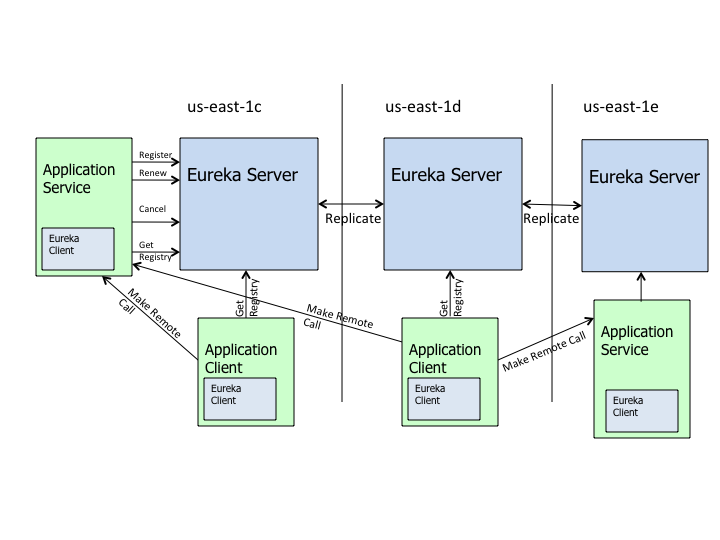
\includegraphics[width=\textwidth, trim={0 4cm 0 0}]{images/netflixEureka/eureka_architecture.png}
    \caption{przykładowa architektura klastra usług Eureka w Netflixie\cite{netflixEurekaGithub}}
    \label{fig:enter-label}
\end{figure}

Powyższa architektura przedstawia sposób, w jaki Eureka jest wdrażana w Netflixie i jest to typowy sposób jej uruchamiania. Na każdy region przypada jedna usługa (bądź też klaster usług) Eureka, w którym rejestrują się instancje z tego regionu, w którym jest uruchomiona. Usługi rejestrują się w serwerze Eureka, a następnie co 30 sekund wysyłają wiadomość hearbeat (\english{heartbeats}), aby odnowić swoje dzierżawy. Jeżeli usługa nie może odnowić dzierżawy kilka razy, jest ona usuwana z rejestru serwera w ciągu około 90 sekund. Informacje o rejestracji i odnowieniach są replikowane na wszystkich węzłach Eureka w klastrze. Klienci z dowolnej strefy mogą wyszukiwać informacje w rejestrze, aby zlokalizować swoje usługi (które mogą znajdować się w innej strefie niż klient) następnie po otrzymaniu informacji o szukanej instancji, klient wykonuje połączenie do usługi\cite{netflixEurekaArticleWang}\cite{netflixEurekaGithub}\cite{springEureka}\cite{netflixEurekaManual}.

\section{Docker}

\begin{figure}[!htbp]
    \centering
    
\includegraphics[width=0.2\textwidth]{images/Docker_logo.png}
    \caption{Logo marki Docker \cite{DockerMedia}}
    \label{fig:enter-label}
\end{figure}

W przeszłości aplikacje były zazwyczaj wdrażane na serwerach fizycznych lub maszynach wirtualnych. Przed wdrożeniem aplikacji należy skonfigurować niezbędną infrastrukturę. Obejmowało to instancję systemu operacyjnego, wszelkich zależności wymaganych przez aplikację i skonfigurowanie wszystkiego by ze sobą współpracowało w prawidłowy sposób. Było to czasochłonne i skomplikowane, zwłaszcza gdy próbowało się odtworzyć dokładnie to środowisko, dla którego aplikacja została stworzona.
Maszyny wirtualne stanowią pod tym względem znaczącą przewagę nad serwerami fizycznymi. Umożliwiają one programistom oddzielenie tworzonego oprogramowania od bazowego systemu. Dodatkowo, oferują one deweloperom łatwo dostępne środowisko, które mogli wykorzystywać do rozwoju i testowania, oddzielone od głównego systemu operacyjnego. Jednak maszyny wirtualne także posiadają swój własny zestaw wyzwań\cite{dockerContenerizationKeyAndUseCases}. 

Jednym z głównych problemów jest to, że wymagają one pełnej kopii systemu operacyjnego. Oznacza to, że są one stosunkowo duże i zajmują dużo zasobów. Z tego powodu uruchamianie wielu maszyn wirtualnych na tym samym serwerze fizycznym jest stosunkowo kosztowne. Nie tylko uruchomienie setek maszyn wirtualnych jest kosztowne, ale także wymaga dużej ilości zasobów, takich jak rdzenie procesora, pamięć \acronym{RAM} (\english{Random Access Memory}) i przestrzeń dyskowa. Co więcej, trudno jest skalować aplikacje w poziomie, co oznacza konieczność dodania większej liczby replik aplikacji w celu obsłużenia zwiększonego ruchu, liczby użytkowników, czy obciążenia pracy danej repliki \cite{dockerContenerizationKeyAndUseCases}.

Konteneryzacja oferuje natomiast szereg korzyści, które pozwalają sprostać tym wyzwaniom. Dzięki konteneryzacji, deweloperzy mogą spakować swoje aplikacje i ich zależności w jednym kontenerze. Obraz Kontenera można natomiast dostarczyć i wdrożyć na dowolnej platformie, która go obsługuje. Ułatwia to wdrożenie i uruchamianie aplikacji w rożnych środowiskach. Konteneryzacja oferuje spójne i niezawodne działanie aplikacji na różnych platformach, niezależnie od tego czy jest to serwer fizyczny, maszyna wirtualna w chmurze, czy też system operacyjny Windows lub Linux\cite{dockerContenerizationKeyAndUseCases}\cite{dockerOverview}. 

Dodatkowymi atutami konteneryzacji są:

\begin{itemize}
    \item \textbf{Przenośność}: Skonteneryzowane aplikacji może łatwo przenieść między różnymi środowiskami. Na przykład, można je łatwo przenieść z laptopa dewelopera do środowiska przejściowego lub produkcyjnego. Nie trzeba martwić się o różne konfiguracje między laptopem a serwerem, na którym zostanie wdrożony kontener\cite{dockerContenerizationKeyAndUseCases}\cite{dockerOverview}.
    
    \item \textbf{Izolacja}: Kontenery zapewniają warstwę izolacji między aplikacją a systemem hosta. Jest to coś w rodzaju bariery ochronnej, która pomaga zapobiegać konfliktom między różnymi aplikacjami lub zależnościami. Każdy kontener działa w swoim własnym, odizolowanym środowisku. Oznacza to, że jest mniej prawdopodobne, że wpłyną na niego inne aplikacje lub procesy działające na tej samej maszynie hosta. W związku z tym znacznie trudniej jest aplikacjom w kontenerach negatywnie wpływać na siebie nawzajem lub na system hosta. Pliki w systemie hosta i w innych kontenerach pozostaną nienaruszone, ponieważ aplikacja nie może uzyskać dostępu do plików spoza własnego środowiska\cite{dockerContenerizationKeyAndUseCases}\cite{dockerOverview}.

    \item \textbf{Wydajność zasobów}: Kontenery umożliwiają uruchamianie wielu odizolowanych aplikacji w tym samym systemie hosta. Nie trzeba przydzielać zasobów do każdej z nich z osobna (jak ma to miejsce w przypadku maszyn wirtualnych). Skutkuje to znacznym zmniejszeniem wykorzystania zasobów i kosztów. Ta zaleta jest szczególnie korzystna w środowiskach chmurowych, gdzie opłaty są często oparte na wykorzystaniu zasobów\cite{dockerContenerizationKeyAndUseCases}\cite{dockerOverview}.

    \item \textbf{Łatwe pakowanie, dostarczanie i wdrażanie}: Dla dewelopera spakowanie aplikacji do obrazu kontenera jest prostym procesem. Następnie deweloper może przesłać zbudowany obraz do rejestru kontenerów, który działa jako scentralizowany serwer do dystrybucji obrazu innym osobom. W ten sposób inne osoby mogą w prosty sposób pobrać zbudowany obraz na swoje urządzenie i go uruchomić\cite{dockerContenerizationKeyAndUseCases}\cite{dockerOverview}.
\end{itemize}

W 2013 roku powstało narzędzie Docker, które znacząco ułatwiło pracę z wykorzystaniem kontenerów. Z wykorzystaniem tego narzędzia można było tworzyć obrazy, przesyłać je do repozytorium, uruchamiać kontenery, łączyć je w sieci i wykonywać wiele innych zadań związanych z kontenerami. Oznacza to, że wystarczy użyć tylko jednego narzędzia aby obsłużyć wszystkie potrzeby związane z kontenerami. W rezultacie kontenery stały się głównym nurtem i zyskały ogromną popularność\cite{dockerContenerizationKeyAndUseCases}\cite{dockerOverview}.

\subsubsection{Docker Compose}

Docker Compose to narzędzie do definiowania i uruchamiania aplikacji wielokontenerowych. Jest to klucz do odblokowania usprawnionego i wydajnego środowiska programowania i wdrażania.
Docker Compose upraszcza kontrolę nad całym stosem aplikacji, ułatwiając zarządzanie usługami, sieciami i wolumenami w jednym, zrozumiałym pliku konfiguracyjnym \akronim{YAML} (\english{YAML Ain’t Markup Language}). Następnie za pomocą jednego polecenia można utworzyć i uruchomić wszystkie usługi z pliku konfiguracyjnego. Compose działa we wszystkich środowiskach: produkcyjnym, przejściowym, deweloperskim, testowym, a także w przepływach pracy \akronim{CI} (\english{Continuous Integration})\cite{dockerComposeAStudyMultiContainerSystem}\cite{dockerComposeOverview}\cite{dockerComposePaterns}.

Docker Compose posiada również polecenia do zarządzania całym cyklem życia aplikacji: 
\begin{itemize}
    \item Uruchamianie, zatrzymywanie i przebudowywanie stosu usług
    \item Wyświetlenie stanu uruchomionych aplikacji
    \item Przesyłanie strumieniowe danych wyjściowych dziennika uruchomionych usług
    \item Uruchamianie jednorazowego polecenia w określonym kontenerze
\end{itemize}

\section{Elasticsearch}

\begin{figure}[!htbp]
    \centering
    \includesvg[width=0.1\textwidth]{images/ELK-Stack/logo-elasticsearch-32-color.svg}
    \caption{Logo Elasticsearch \cite{elasticSearchManualDataIn}}
    \label{fig:enter-label}
\end{figure}

Elasticsearch to rozproszony magazyn dokumentów. Zamiast przechowywać informacje w postaci encji, Elasticsearch przechowuje złożone struktury danych, które zostały serializowane jako dokumenty \akronim{JSON} (\english{JavaScript Object Notation}). W przypadku posiadania wielu węzłów Elasticsearch w klastrze, przechowywane dokumenty są dystrybuowane w całym klastrze i można uzyskać do nich natychmiastowy dostęp z dowolnego węzła\cite{elasticSearchManualDataIn}. 

Elasticsearch jest zbudowany tak, aby był zawsze dostępny i skalował się zgodnie z wymaganiami systemu w którym pracuje. Osiąga to dzięki swojej rozproszonej naturze. Dodając węzły do klastra zwiększa się jego pojemność a następnie Elasticsearch automatycznie rozdzieli dane i obciążenie na wszystkie dostępne węzły. Nie ma potrzeby przebudowywania aplikacji, Elasticsearch sam zrównoważy klastry wielowęzłowe, aby zapewnić wysoką dostępność.

Gdy dokument jest przechowywany w systemie, jest indeksowany i w pełni przeszukiwalny. Elasticsearch wykorzystuje strukturę danych zwaną odwróconym indeksem, który obsługuje bardzo szybkie wyszukiwanie pełnotekstowe. Odwrócony indeks wyszczególnia każde unikalne słowo, które pojawia się w dowolnym dokumencie i identyfikuje wszystkie dokumenty, w których każde słowo występuje\cite{elasticSearchManualDataIn}.  

Indeks można traktować jako zoptymalizowaną kolekcję dokumentów, a każdy dokument jest zbiorem pól, które są parami klucz--wartość zawierającymi dane. Domyślnie Elasticsearch indeksuje wszystkie dane w każdym polu, a każde indeksowane pole ma dedykowaną, zoptymalizowaną strukturę danych.
Na przykład pola tekstowe są przechowywane w indeksach odwróconych, a pola numeryczne i geograficzne są przechowywane w drzewach \akronim{BKD}. Zdolność do korzystania ze struktur danych dla poszczególnych typów pól do gromadzenia i zwracania wyników wyszukiwania sprawia, że Elasticsearch jest w stanie szybko przetwarzać dane\cite{elasticSearchManualDataIn}.

Elasticsearch ma również możliwość nieposiadania, z góry predefiniowanego schematu, co oznacza że dokumenty mogą być indeksowane bez wyraźnego określenia sposobu obsługi każdego z pól, które mogą wystąpić w dokumencie. Gdy dynamiczne mapowanie jest włączone, Elasticsearch automatycznie wykrywa i dodaje nowa pola do indeksu. To domyślne zachowanie ułatwia indeksowanie i eksplorację danych, w momencie indeksowania, Elasticsearch wykrywa i mapuje wartości logiczne, zmiennoprzecinkowe, całkowite, daty i ciągi znaków na odpowiednie typy danych\cite{elasticSearchManualDataIn}. 

Ostatecznie jednak użytkownik wie więcej o swoich danych i sposobie ich wykorzystania niż Elasticsearch. Użytkownik może zdefiniować reguły kontrolujące dynamiczne mapowanie i jawnie zdefiniować konwersję, aby przejąć pełną kontrolę nad sposobem przechowywania i indeksowania pól\cite{elasticSearchManualDataIn}.

Definiowanie własnych mapowań umożliwia:

\begin{itemize}
    \item Rozróżnianie pełnotekstowych pól łańcuchowych i pól łańcuchowych z dokładną wartością.
    \item Przeprowadzanie analizy tekstu specyficznej dla języka
    Optymalizację pól pod kątem częściowego dopasowywania
    \item Używanie niestandardowych formatów daty
    \item Używanie typów danych, takich jak \verb|geo_point| i \verb|geo_shape|, których nie można wykryć automatycznie.
\end{itemize}

Często przydatne jest indeksowanie tego samego pola na różne sposoby w różnych celach. Na przykład, użytkownik może chcieć indeksować pole łańcuchowe zarówno jako pole tekstowe do wyszukiwania pełnotekstowego, oraz jako pole słów kluczowych do sortowania lub agregowania danych. Można też użyć więcej niż jednego analizatora języka do przetworzenia zawartości pola łańcuchowego zawierającego dane wejściowe użytkownika\cite{elasticSearchManualDataIn}.

\section{Logstash}

\begin{figure}[!htbp]
    \centering
    \includesvg[width=0.1\textwidth]{images/ELK-Stack/logo-logstash-32-color.svg}
    \caption{Logstash logo\cite{logstashMain}}
    \label{fig:enter-label}
\end{figure}

Logstash to silnik gromadzenia danych typu otwarto źródłowego (\english{Open source}) z możliwością potokowania w czasie rzeczywistym. Logstash może dynamicznie ujednolicić dane z różnych śródeł i normalizować je do wybranych miejsc docelowych. Oczyszcza i demokratyzuje wszystkie dane dla różnorodnych zaawansowanych zastosować analiztycznych i wizualizacyjnych\cite{logstashManualIntroduction}.

Logstash pierwotnie napędzał innowacje w zakresie gromadzenia logów, jego możliwości wykraczają dlatego poza ten przypadek użycia. Każdy rodzaj zdarzenia można wzbogacić i przekształcić za pomocą szerokiej gamy wtyczek wejściowych, filtrujących i wyjściowych, a wiele natywnych kodeków dodatkowo upraszcza proces pozyskiwania danych. Logstash przyspiesza pozyskiwanie informacji poprzez wykorzystanie większej ilości i różnorodności danych\cite{logstashManualIntroduction}.

Potok przetwarzania zdarzeń Logstash składa się z trzech etapów:

\begin{figure}[!htbp]
    \centering
    \includesvg[width=0.15\textwidth]{schemas/logstashPipeline.drawio.svg}
    \caption{Przetwarzanie zdarzeń w logstash}
    \label{fig:enter-label}
\end{figure}

Wejścia generują zdarzenia, następnie są one filtrowane aby ostatecznie wyjścia wysłały je do miejsca docelowego. Wejścia i wyjścia obsługują kodeki, które umożliwiają kodowanie lub dekodowanie danych wchodzących lub wychodzących z potoku bez konieczności  stosowania oddzielnego filtra\cite{logstashManualHowItWorks}. 

\subsubsection{Wejścia}

Wejścia służą do pobierania danych do Logstash. Niektóre z najczęściej używanych wejść to:

\begin{itemize}
    \item file: odczyt z pliku w systemie plików, podobnie jak w polecenie w UNIX \termdef{tail -0F}\cite{logstashManualHowItWorks}.
    \item syslog: nasłuchuje na porcie 514 i analizuje je zgodnie z formatem RFC3164\cite{rfc3164}\cite{logstashManualHowItWorks}.
    \item redis: oczytuje z serwera redis, używając zarówno kawałków oraz list. Redis jest często używany jako "broker" w scentralizowanym systemie. Logstash, który kolejkuje zdarzenia od zdalnych nadawców\cite{logstashManualHowItWorks}.
    \item beats: przetwarza zdarzenia wysłane przez Beats\cite{logstashManualHowItWorks}.
\end{itemize}

\subsubsection{Filtry}

Filtry są pośrednimi urządzeniami przetwarzającymi w potoku. Filtry można łączyć z instrukcjami warunkowymi w ceu wykonania akcji na zdarzeniu, jeśli spełnia ono określone kryteria. Niektóre przydatne filtry obejmują: 

\begin{itemize}
    \item \textbf{grok}: parsuje i strumieniuje dowolny tekst. Grok jest obecnie najlepszym sposobem w Logstash na analizowanie nieustrukturyzowanych danych dziennika w celu przetworzenia danych w formę nadającą się do zapytań\cite{logstashManualHowItWorks}. 
    \item \textbf{mutate}: wykonuje ogólne transformacje na polach zdarzeń. Można edytować nazwy, usuwać, zastępować i modyfikować pola w zdarzeniach.
    \item \textbf{drop}: pozwala na całkowicie odrzucenie zdarzenia\cite{logstashManualHowItWorks}.
    \item \textbf{clone}: tworzy kopię zapasową zdarzenia, ewentualnie dodając lub usuwając pola\cite{logstashManualHowItWorks}.
    \item \textbf{geoip}: dodawanie informacji o położeniu geograficznym adresów IP\cite{logstashManualHowItWorks}.
\end{itemize}

\subsubsection{Wyjścia}

Wyjścia są ostatnią fazą potoku Logstash. Zdarzenie może przechodzić przez wiele wyjść, ale po zakończeniu przetwarzania wszystkich danych wyjściowych zdarzenie kończy swoje wykonanie\cite{logstashManualHowItWorks}.
Niektóre często używane wyjścia obejmują:

\begin{itemize}
    \item \textbf{elasticsearch}: wysyła dane zdarzeń do Elasticsearch\cite{logstashManualHowItWorks}.
    \item \textbf{file}: zapisywanie danych zdarzeń do pliku na dysku\cite{logstashManualHowItWorks}.
    \item \textbf{graphite}: wysyła dane do zdarzeń do graphite, popularnego otwarto źródłowego narzędzia do przechowywania i tworzenia wykresów metryk\cite{logstashManualHowItWorks}.
\end{itemize}

\subsubsection{Kodeki}

Kodeki to filtry strumieniowe, które mogą działać jako część wejścia lub wyjścia. Kodeki umożliwiają łatwe oddzielenie transportu wiadomości od procesu serializacji. Do najpopularniejszych kodeków należą:

\begin{itemize}
    \item \textbf{json}: koduje lub dekoduje dane w formacie JSON\cite{logstashManualHowItWorks}.
    \item \textbf{multiline}: łączy wielowierszowe zdarzenia tekstowe, takie jak wyjątki w javia i komunikaty zrzutem stosu (\english{Stack trace}) w jedno zdarzenie\cite{logstashManualHowItWorks}.
\end{itemize}

\section{Metricbeat}


\begin{figure}[!htbp]
    \centering
    \includesvg[width=0.1\textwidth]{images/ELK-Stack/icon-metricbeat-32-color.svg}
    \caption{Logo Metricbeat\cite{metricbeatLogo}}
    \label{fig:enter-label}
\end{figure}

Metricbeat to program wykorzystywany do okresowego zbierania metryk z systemu operacyjnego i usług działających na serwerze. Metricbeat pobiera zebrane metryki i statystyki a następnie wysyła je do okreslonych przez użytkownika punktów docelowych, takich jak Elasticsearch, Logstash, Redis lub Kafka\cite{metricbeatOverview}.


\section{Kibana}

\begin{figure}[!htbp]
    \centering
    \includesvg[width=0.1\textwidth]{images/ELK-Stack/logo-kibana-32-color.svg}
    \caption{Logo Kibana\cite{kibanaLogo}}
    \label{fig:enter-label}
\end{figure}

Kibana jest to narzędzie do wizualizacji i eksploracji danych wykorzystywane do analizy dokumentów, przechowywanych w stosie oprogramowania Elastic. Kibana umożliwia nadanie kształtu danym oraz poruszanie się po stosie oprogramowania Elastic\cite{kibanaOverview}. 

Kibana między innymi zapewnia następujące funkcjonalności:

\begin{itemize}
    \item \textbf{Wyszukiwanie, obserwowanie i chronienie danych}: Odkrywanie dokumentów,  analizowanie dzienników oraz znajdowanie luk w zabezpieczeniach\cite{kibanaOverview}.
    \item \textbf{Analiza danych}: Wyszukiwanie zależności, wizualizacja danych na grafach, diagramach, mapach oraz tworzenie, pulpitów nawigacyjnych\cite{kibanaOverview}.
    \item \textbf{Monitoring}: Kibana zapewnia możliwość monitorowania całego klastra oprogramowania Elastic oraz kontrolowania dostępu użytkowników do poszczególnych funkcjonalności\cite{kibanaOverview}.
\end{itemize}

\section{Logstash Logback Encoder}

Logstash Logback Encoder to biblioteka zaprojektowana w celu ułatwienia rejestrowania dzienników aplikacji w formacie JSON przy użyciu biblioteki Logback. Koder ten umożliwia ustrukturyzowanie przechowywanie zdarzeń w formacie JSON, ułatwiając analizowanie dzienników przy wykorzystaniu takich narzędzi jak Logstash i Elasticsearch\cite{logstashLogbackEncoderOverview}. 

Kluczowe cechy:

\begin{itemize}
    \item \textbf{Kodowanie JSON}: Podstawową funkcją tego kodera jest kodowanie zdarzeń Logback do formatu JSON\cite{logstashLogbackEncoderOverview}.
    \item \textbf{Konfigurowalny wygląd}: Biblioteka pozwala na dostosowanie układów logów, umożliwiając użytkownikom zdefiniowanie własnej struktury zdarzeń\cite{logstashLogbackEncoderOverview}.
    \item \textbf{Zaawansowane dodatki}: Dodatkowe appendery, takie jak LogstashTcpSocketAppender i AsyncDisruptorAppender, które ułatwiają wysyłanie logów przez sieć lub ich asynchroniczną obsługę\cite{logstashLogbackEncoderOverview}.
    \item \textbf{Wsparcie dla filtrów Logback}: Biblioteka obsługuje filtry Logback, umożliwiając warunkowe logowanie w oparciu o niestandardowe kryteria\cite{logstashLogbackEncoderOverview}.
    \item \textbf{Maskowanie i zmiana}: Wrażliwe informacje w dziennikach mogą być maskowane lub zmieniane w celu zapewnienia zgodności z przepisami dotyczącymi prywatności danych\cite{logstashLogbackEncoderOverview}.
\end{itemize}

Biblioteka jest szczególnie wykorzystywana w systemach rozproszonych do centralizacji dzienników aplikacyjnych z wielu źródeł i usprawniania ich analizy za pomocą narzędzi takich jak stos \akronim{ELK} (Elasticsearch, Logstash, Kibana)\cite{logstashLogbackEncoderOverview}.

Aby zintegrować Logstash Logback Encoder z projektem Java, należy uwzględnić go jako zależność w konfiguracji kompilacji w pliku konfiugracyjnym, dodatkowo należy skonfigurować plik \textit{logback-spring.xml}, tak aby biblioteka korzystała z prawidłowych appenderów\cite{logstashLogbackEncoderOverview}.
\chapter{Implementacja}

Niniejszy rozdział zawiera szczegółowe omówienie sposobu implementacji zaproponowanego systemu. Poniższy opis obejmuje konfigurację komponentów, integrację mechanizmów wykrywania usług i zarządzania zasobami oraz konfigurację narzędzi do monitorowania. Analizując te aspekty implementacji, rozdział ujawnia, w jaki sposób realizowana jest architektura systemu, umożliwiając dynamiczną interakcję między producentami i użytkownikami, efektywną alokację zasobów i monitorowanie wydajności systemu.

\section{Podsystem użytkowy}
\subsection{Rejestr usług}

Głównym elementem w podsystemie użytkowym jest rejestr usług, rejestr ten jest wykorzystywany jako zbiór informacji na temat usług uruchomionych w systemie. W usłudze następuje rejestracja producentów świadczący usługi w systemie oraz węzłów protokołu użytkowników, które są wykorzystywane do zarządzania przydziałem zasobów.

\begin{figure}[!htbp]
    \centering
    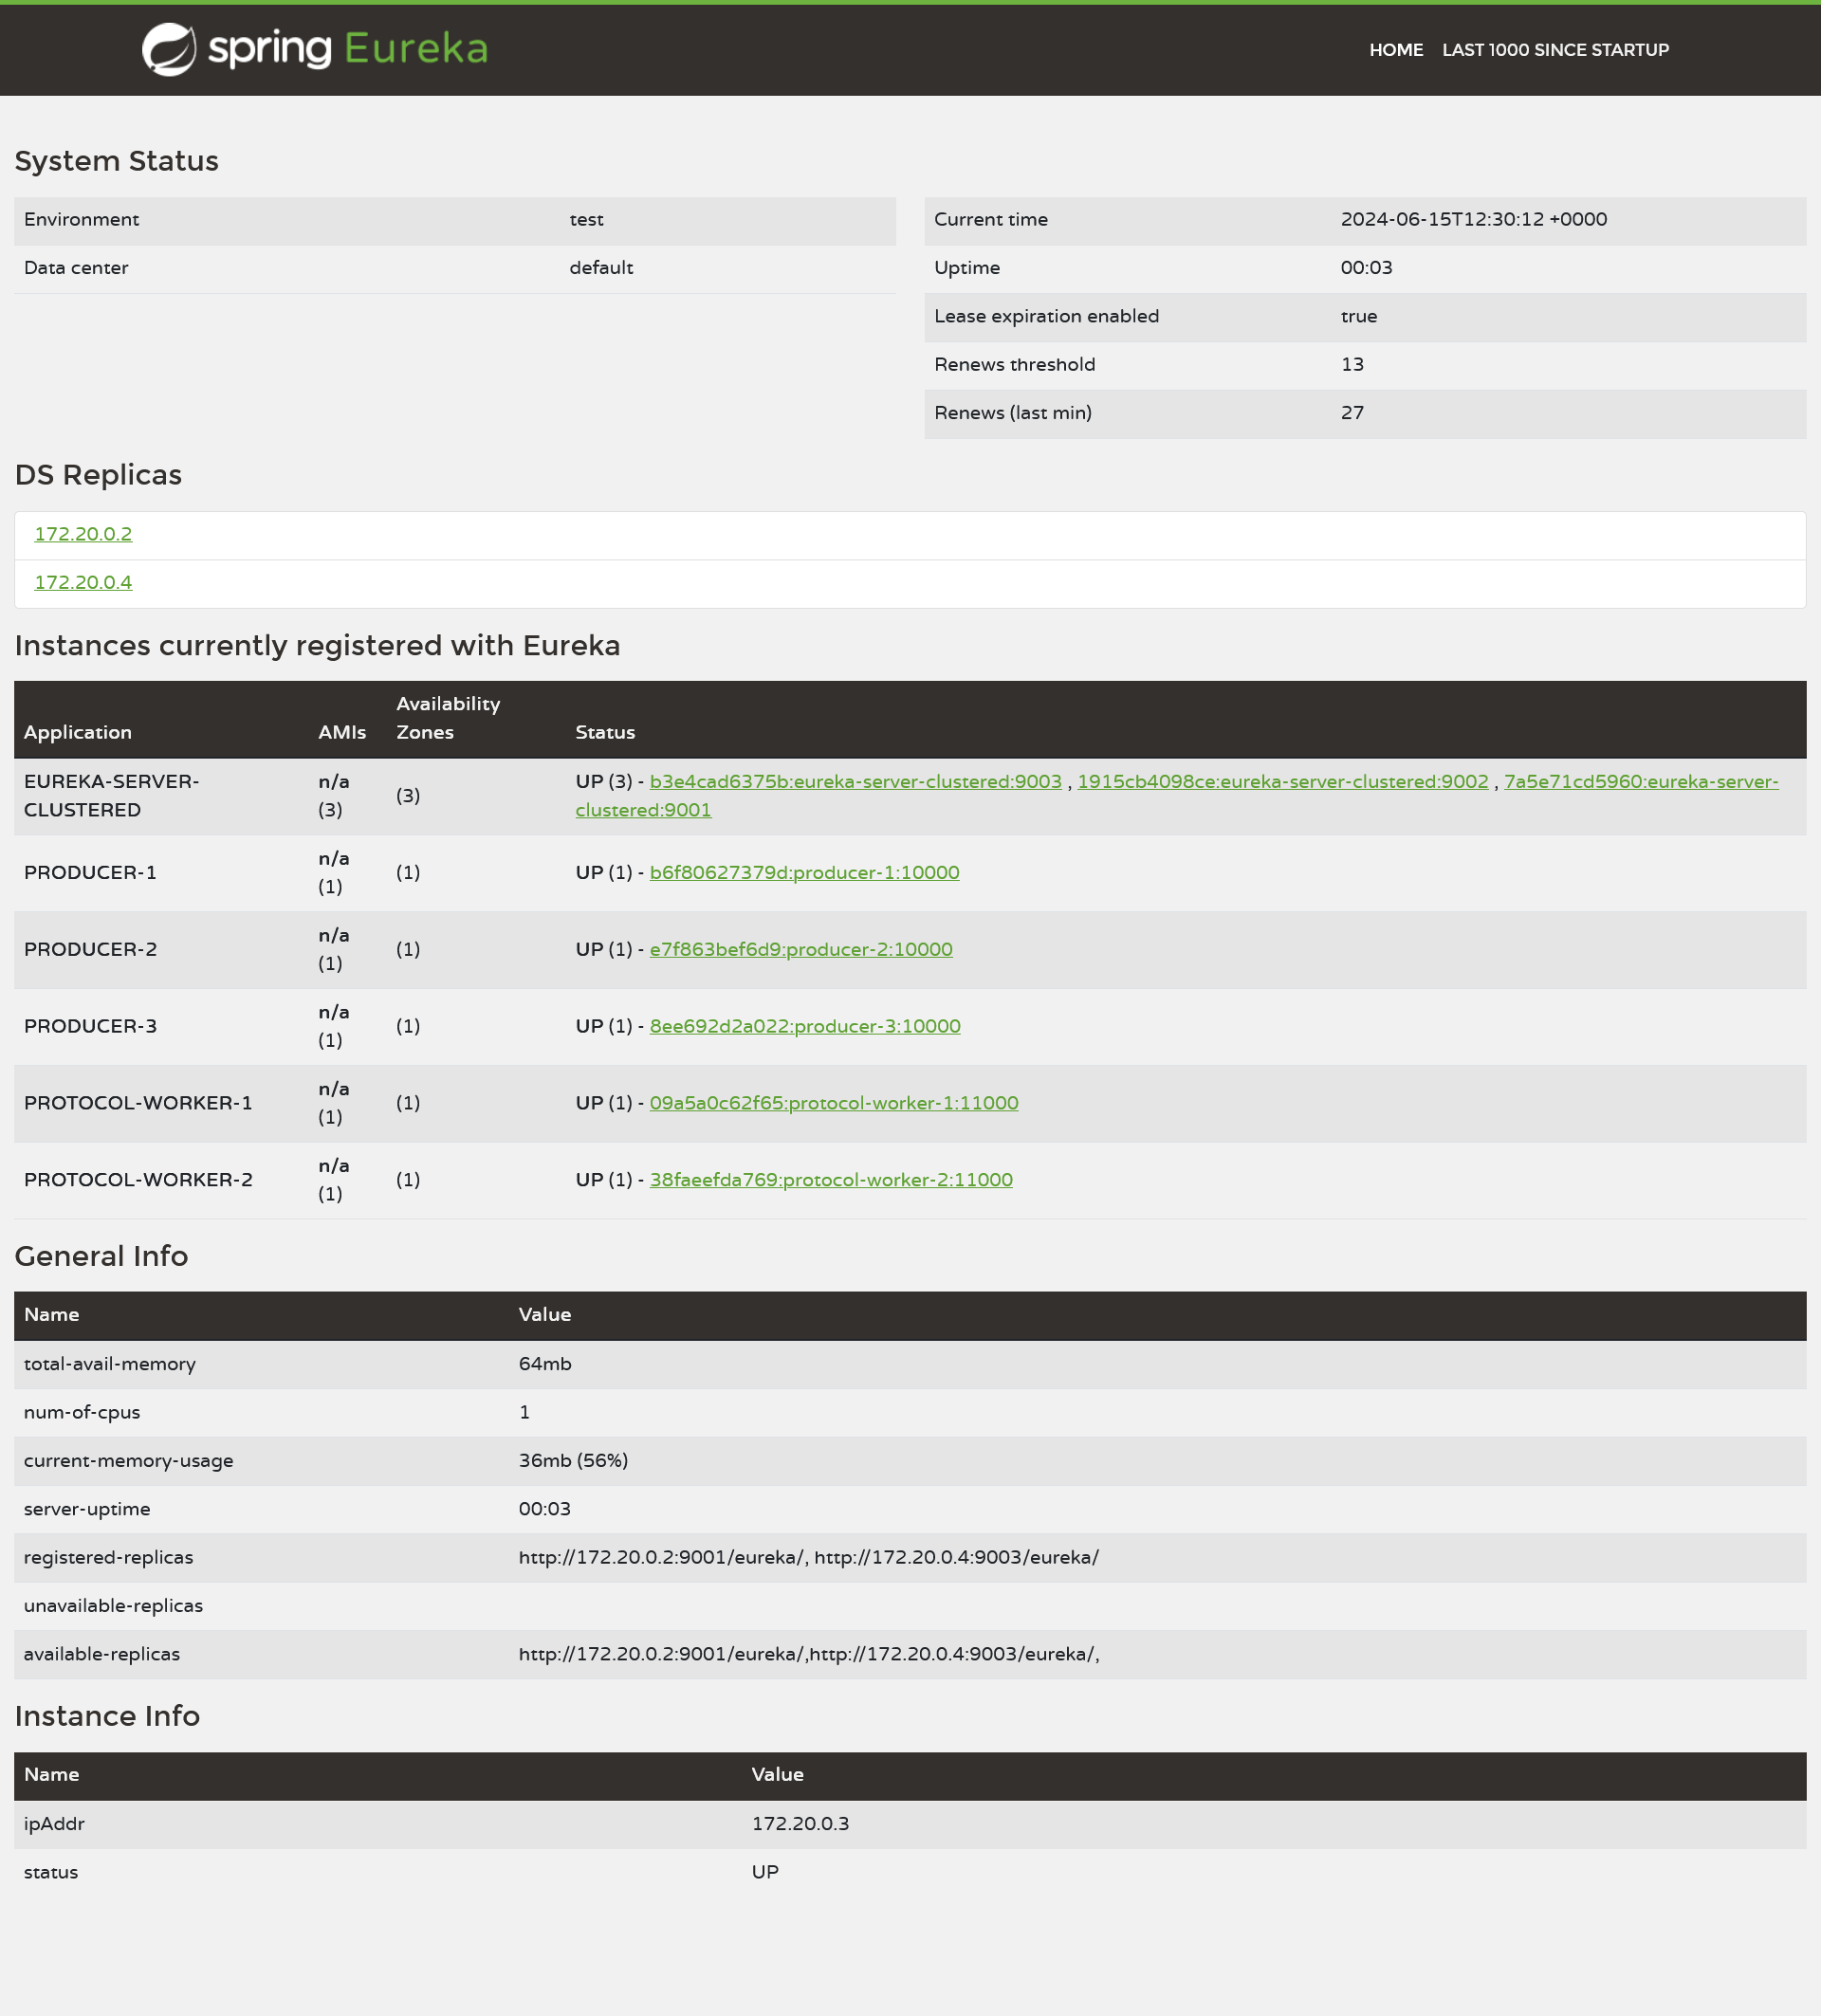
\includegraphics[width=\textwidth]{images/implementation/ServerDiscovery3Producer2Workers.png}
    \caption{Rejestr usług Eureka}
    \label{eurekaServerItems}
\end{figure}

Każda uruchomiona usługa typu producenta oraz węzła protokołu w podsystemie użytkowym jest rejestrowana w usłudze Eureka, gdzie aplikacja przechowywana jest pod unikalną nazwą, która jest wykorzystywana do odpytywania rejestru w usłudze klienckiej w celu otrzymania informacji o działających usługach w systemie. Rejestr przechowuje adres pod którym usługa jest uruchomiona oraz jej stan. Na rys.\ref{eurekaServerItems} jest przedstawiony przykładowy stan usług zarejestrowanych w rejestrze Eureka.

\begin{lstlisting}[language=Java, caption=Implementacja rejestru usług serwera Eureka]
    
    package com.example.serviceregistry;
    
    import org.springframework.boot.SpringApplication;
    import org.springframework.boot.autoconfigure.SpringBootApplication;
    import org.springframework.cloud.netflix.eureka.server.EnableEurekaServer;
    
    
    @SpringBootApplication
    @EnableEurekaServer
    public class ServiceRegistryApplication {
    
    	public static void main(String[] args) {
    		SpringApplication.run(ServiceRegistryApplication.class, args);
    	}
    }
\end{lstlisting}

Kod usługi rejestru składa się z jednej klasy \verb|ServiceRegistryApplication| oraz metody \verb|main| uruchamiającej aplikacje. Jedyną linijką odróżniającą tę klasę od czystej aplikacji napisanej w frameworku Spring Boot jest adnotacja \verb|@EnableEurekaServer|(linia 10), odpowiada ona za uruchomienie usługi Eureka.

Głównym elementem określającym działanie usługi jest profil Spring Boot oraz wartości przypisane temu profilowi w pliku \verb|application.yml|. 

\subsubsection{Konfiguracja węzła rejestru}

Plik konfiguracyjny \verb|application.yml| jest plikiem YAML podzielony na trzy sekcje, każda opisująca oddzielny profil aplikacji oraz  pola konfiguracyjne niezbędne do prawidłowego działania klastra węzłów rejestru Eureka. 

\begin{lstlisting}[caption=Konfiguracja pierwszego węzła rejestru]
    spring:
      config:
        activate:
          on-profile: peer-1
      application:
        name: eureka-server-clustered
    server:
      port: 9001
    eureka:
      instance:
        preferIpAddress: true
        leaseRenewalIntervalInSeconds: 10
        leaseExpirationDurationInSeconds: 30
      client:
        registerWithEureka: true
        fetchRegistry: true
        serviceUrl:
          defaultZone: ${PEER_2_URL:http://localhost:9002/eureka/},${PEER_3_URL:http://localhost:9003/eureka/}
      server:
        enableSelfPreservation: true
        evictionIntervalTimerInMs: 1000
    logging:
      logstash:
        destinationOne: ${LOGSTASH_DESTINATION_ONE:localhost:5000}
        destinationTwo: ${LOGSTASH_DESTINATION_TWO:localhost:5001}
        destinationThree: ${LOGSTASH_DESTINATION_THREE:localhost:5002}
\end{lstlisting}

\subsubsection{Konfiguracja aplikacji}

Pole \verb|spring.config.activate.on-profile|(linia 4) określa, który profil aplikacyjny będzie aktywny podczas inicjalizacji usługi.

Pole \verb|spring.application.name| (linia 6) ustawia nazwę aplikacji na eureka-server-clustered. Nazwa ta jest wykorzystywana do identyfikacji oraz rejestracji aplikacji w klastrze Eureka.

Pole \verb|server.port| (linia 8) określa port urządzenia na którym aplikacja ma być uruchomiona.

\subsubsection{Konfiguracja instancji Eureka}

Pole \verb|eureka.instance.preferIpAddress| (linia 11) wartość tego pola ustawiona na \verb|true| określa preferowanie przez Eureka adresu \akronim{IP} (\english{Internet Protocol}) zamiast nazwy urządzenia do rejestrowania usług.

Pole \verb|eureka.instance.leaseRenewalIntervalInSeconds| (linia 12) ustawia interwał(w sekundach), co który instancja będzie wysyłać informacje o chęci odnowienia dzierżawy.

Pole \verb|eureka.instance.leaseExpirationDurationInSeconds| (linia 13) określa czas trwania(w sekundach), po którym instancja usługi zostanie uznana za wyłączoną, jeżeli aplikacja nie odnowi dzierżawy.

\subsubsection{Konfiguracja klienta Eureka}

Pole \verb|eureka.client.registerWithEureka| (linia 15) wskazuje, że instancja powinna zarejestrować się w serwerze Eureka.

Pole \verb|eureka.client.fetchRegistry| (linia 16) określa, czy ta instancja powinna pobrać informację z rejestru Eureka.

Pole \verb|eureka.client.serviceUrl.defaultZone| (linia 18) określa adresy \akronim{URL} (\english{Uniform Resource Locator}) usług równorzędnych serwerów Eureka w klastrze.

\subsubsection{Konfiguracja serwera Eureka}

Pole \verb|eureka.server.enableSelfPreservation| (linia 20) określa tryb samozachowawczy, który pomaga w utrzymaniu dostępności serwera Eureka nawet w przypadku partycji sieciowej lub dużych opóźnień.

Pole \verb|eureka.server.evictionIntervalTimerInMs| (linia 21) ustawia interwał (w milisekundach), dla którego ma być uruchamiane zadanie usuwania aplikacji których czas dzierżawy wygasł.

\subsubsection{Konfiguracja logowania zdarzeń}

Pola \verb|logging.logstash.destination*| (linie 24-26) ustawiają adres do usług zbierających dokumenty, do których będą wysyłane informacje o zdarzeniach w aplikacji producenta. Wykorzystuje zmienną środowiskową LOGSTASH\_DESTINATION\_*, która domyślnie jest ustawiona na localhost:5000, jeśli nie zostanie podana przy uruchomieniu aplikacji.\\[0.5cm]

plik \verb|application.yml| definiuje ustawienia konfiguracyjne dla aplikacji Spring Boot z różnymi profilami: peer-1, peer-2 i peer-3. Każdy profil konfiguruje aplikację jako część klastrowej konfiguracji serwera Eureka oraz wykorzystuje pozostałe uruchomione serwery Eureka jako repliki swojego rejestru w celu zapewnienia wysokiej dostępności w przypadku awarii jednego z węzłów w klastrze.

\subsection{Producent}

Producenci w systemach rozproszonych to komponenty lub usługi odpowiedzialne za generowanie i dostarczanie produktów lub danych. Służą jako źródło informacji lub towarów, które następnie są konsumowane przez inne części systemu. W przedstawianym systemie diagram klas usługi producenta został przedstawiony na rys\ref{ProducerUML}.

\begin{figure}[!htbp]
    \centering
    \includesvg[width=0.65\textwidth]{schemas/producer/Producer.drawio.svg}
    \caption{Producent - schemat UML}
    \label{ProducerUML}
\end{figure}

\subsubsection{Wymagania funkcjonalne}

Usługa producenta powinna spełniać następujące wymagania funkcjonalne:

\begin{itemize}
    \item Producent powinien sprawdzać czy dany produkt znajduje się w jego ofercie.
    \item Producent powinien sprawdzać czy ilość produktów zamawianych przez klienta jest możliwa przez niego do spełnienia. 
    \item Producent powinien zapewnić możliwość odbioru danych w celu sprawdzenia szybkości transmisji między nim a użytkownikiem.
\end{itemize}


\subsubsection{Główna klasa usługi producenta}

Główna klasa usługi producenta przedstawiona na rys\ref{producerMainClass}, jest podstawową klasą uruchamiającą aplikację z wykorzystaniem frameworku Spring Boot. Jest ona oznaczona adnotacją \verb|@EnableDiscoveryClient| (linia 8), która zapewnia uruchomienie klienta Eureka w celu rejestracji w serwerze Eureka. Adres serwera na, którym aplikacja ma się zarejestrować ładowany jest z konfiguracji aplikacji.

\begin{lstlisting}[caption=Główna klasa usługi producenta, label=producerMainClass]
    package com.example.producer;

    import org.springframework.boot.SpringApplication;
    import org.springframework.boot.autoconfigure.SpringBootApplication;
    import org.springframework.cloud.client.discovery.EnableDiscoveryClient;
    
    @SpringBootApplication
    @EnableDiscoveryClient
    public class ProducerApplication {
    
        public static void main(String[] args) {
            SpringApplication.run(ProducerApplication.class, args);
        }
    
    }
\end{lstlisting}

\subsubsection{Model produktu}

Klasa \verb|Product| przedstawiona na rys\ref{produktmodel} reprezentuje centralną jednostkę w ramach usługi Producenta.

\begin{lstlisting}[caption=Klasa reprezentująca produkt, label=produktmodel]
    package com.example.producer.model;
    
    import lombok.AllArgsConstructor;
    import lombok.Getter;
    import lombok.NoArgsConstructor;
    import lombok.Setter;
    
    @Getter
    @Setter
    @AllArgsConstructor
    @NoArgsConstructor
    public class Product {
        String id;
        String name;
        String model;
        String producer;
        Integer amount;
        Integer price;
    
        @Override
        public String toString(){
            return "[id = "+
                    id+
                    ", name=" +
                    name +
                    ", model=" +
                    model +
                    ", producer=" +
                    producer +
                    ", amount=" +
                    amount +
                    "price=" +
                    price +
                    "]";
        }
    
    }
\end{lstlisting}

Klasa ta jest opatrzona adnotacjami Lombok (linie 8-11), \verb|@Getter|, \verb|@Setter|, które pozwalają automatycznie wygenerować funkcję dostępowe do zmiennych znajdujących się w klasie.

Klasa ta zawiera następujące zmienne:
\begin{itemize}
    \item \verb|String id| --- Unikatowe dla danego typu produktu Id (linia 13)
    \item \verb|String name| --- Nazwa produktu (linia 14)
    \item \verb|String model| --- Model produktu (linia 15)
    \item \verb|String producer| --- Nazwa producenta produktu (linia 16)
    \item \verb|Integer amount| --- ilość produktu oferowana przez producenta (linia 17)
    \item \verb|Integer price| --- cena produktu (linia 18)
\end{itemize}

Klasa ta zawiera metodę \verb|toString()| (linie 20-35) która przeciąża domyślną metodę klasową języka java \verb|toString()| aby zapewnić reprezentację obiektu produktu, która zawiera wszystkie atrybuty obiektu.

\subsubsection{Serwis Produktów --- ProductService}

Klasa \verb|ProductsService| zaprezentowana na listingu.\ref{productsServiceCode} jest usługą Spring odpowiedzialną za zarządzanie produktami w aplikacji producenta. Wykorzystuje ona klasę \verb|Product| w celu zainicjowania produktów, przechowywania produktów, oraz pobierania informacji o produktach. Klasa jest opatrzona adnotacją \verb|@Service| (linia 20), wskazującej że jest to komponent usługi Spring, oraz \verb|@Slf4j| (linia 21), aby umożliwić tworzenie dziennika zdarzeń w aplikacji.

\begin{lstlisting}[caption=Kod klasy ProductsService, label=productsServiceCode]
    package com.example.producer.service;

    import com.example.producer.model.Product;
    import com.fasterxml.jackson.core.type.TypeReference;
    import com.fasterxml.jackson.databind.ObjectMapper;
    import jakarta.annotation.PostConstruct;
    import lombok.extern.slf4j.Slf4j;
    import org.springframework.beans.factory.annotation.Value;
    import org.springframework.core.io.ClassPathResource;
    import org.springframework.stereotype.Service;
    
    import java.io.IOException;
    import java.io.InputStream;
    import java.util.ArrayList;
    import java.util.Collections;
    import java.util.List;
    import java.util.Optional;
    import java.util.stream.Collectors;
    
    @Service
    @Slf4j
    public class ProductsService {
    
        @Value("${products.file.name}")
        private String productFileName;
    
        @Value("${products.count}")
        private Integer count;
        private List<Product> products = new ArrayList<>();


        @PostConstruct
        public void loadProducts(){
            ObjectMapper objectMapper = new ObjectMapper();
            List<Product> tempProducts;
            try{
                ClassPathResource resource = new ClassPathResource(this.productFileName);
                InputStream in = resource.getInputStream();
                tempProducts = objectMapper.readValue(in, new TypeReference<List<Product>>(){} );
            }catch (IOException e) {
                log.error("Producer was unable to read products from file");
                throw new RuntimeException("Producer was unable to read products from file", e);
            }
            Collections.shuffle(tempProducts);
            this.products = tempProducts.stream().limit(this.count).collect(Collectors.toList());
        }

        public List<Product> getAllProducts() {
            return products;
        }

        public Optional<Product> getProductByName(Product product) {
            return products.stream().filter(listProduct ->  product.getId().equals(listProduct.getId())  && product.getAmount()<= listProduct.getAmount()).findAny();
        }
    }
\end{lstlisting}

Klasa \verb|ProductsService| zawiera następujące zmienne:
\begin{itemize}
    \item \verb|productFileName| --- Nazwa pliku przechowującego produktu, z którego są ładowane dane przy starcie aplikacji (linia 25). Wartość ta jest wstrzykiwana z konfiguracji aplikacji przy użyciu adnotacji \verb|@Value| (linia 24).
    \item \verb|count| ---  Liczba całkowita określająca liczbę produktów do załadowania (linia 28). Ta wartość jest również wstrzykiwana z konfiguracji aplikacji.
    \item \verb|products| --- Lista obiektów \verb|Product| zawierająca załadowane produkty (linia 29).
\end{itemize}

Klasa \verb|ProductsService| zawiera następujące metody:
\begin{itemize}
    \item \verb|loadProducts| --- Metoda (linie 33-46) opatrzona adnotacją \verb|@PostConstruct| (linia 32) zostaje wywołana automatycznie po inicjalizacji komponentu \verb|ProductsService|. Ładuje ona dane produktów z pliku znajdującego się w głównym folderze aplikacji. Następnie tablica jest mieszana w celu zapewnienia różnych produktów przy każdorazowym uruchomieniu aplikacji. Następnie tablica jest ograniczana do ilości produktów określonej w zmiennej \verb|count|.
    \item \verb|getAllProducts| --- Metoda (linie 48-50) zwracająca wszystkie produkty przechowywane w tablicy \verb|products|.
    \item \verb|getProductByName| --- Metoda (linie 52-54)  przyjmuje obiekt klasy \verb|Product| jako parametr i zwraca obiekt tej samej klasy opatrzony dodatkową klasą\verb|Optional<>|, który może służyć jako tymczasowy pojemnik z pustą wartość w momencie gdy szukany produkt nie zostanie znaleziony u producenta. W momencie wywołania funkcji tablica jest filtrowana w celu znalezienia czy produkt znajduje się w ofercie producenta oraz czy jego ilość spełnia szukane kryterium przesłane w obiekcie wejściowym.
\end{itemize}

\subsubsection{Kontroler prędkości transmisji --- SpeedTestController}

Klasa \verb|speedTestController| przedstawiona na listingu.\ref{speedTestControllerCode} zapewnia punkt końcowy (linia 12) do testowania szybkości połączenia pomiędzy producentem a klientem poprzez odbieranie tablicy bajtów (linia 16) i zwracanie bieżącego czasu systemowego w nanosekundach (linia 18). Punkt końcowy jest mapowany na \verb|/connectionSpeed| i obsługuję żądania \akronim{POST} protokołu \akronim{HTTP} (\english{Hypertext Transfer Protocol}).

\begin{lstlisting}[caption=Kod klasy SpeedTestController, label=speedTestControllerCode]
    package com.example.producer.controllers;

    import lombok.extern.slf4j.Slf4j;
    import org.springframework.http.ResponseEntity;
    import org.springframework.web.bind.annotation.PostMapping;
    import org.springframework.web.bind.annotation.RequestBody;
    import org.springframework.web.bind.annotation.RequestMapping;
    import org.springframework.web.bind.annotation.RestController;
    
    @Slf4j
    @RestController
    @RequestMapping("/connectionSpeed")
    public class SpeedTestController {
    
        @PostMapping
        public ResponseEntity<Long> testSpeed(@RequestBody byte[] data){
            log.info("Received connection speed request, size: {} bytes", data.length);
            return ResponseEntity.ok().body(System.nanoTime());
        }
    }
\end{lstlisting}

\subsubsection{Konfiguracja usługi producenta}

Plik konfiguracyjny przedstawiony na listingu.\ref{producerconfigFIle} służy do konfiguracji usługi producenta. Konfiguruje on właściwości aplikacji, ustawienia serwera, konfigurację klienta Eureka, konfigurację dziennika zdarzeń, szczegóły pliku produktów i punkty końcowe zarządzania.

\begin{lstlisting}[caption=Plik konfiguracyjny usługi producenta, label=producerconfigFIle]
    spring:
      application:
        name: producer-${PRODUCER_ID:producer-ERROR}
      servlet:
        multipart:
          max-file-size: 200MB
          max-request-size: 200MB
    
    server:
      port: ${PORT:10000}
      tomcat:
        max-swallow-size: 209715200
        max-http-form-post-size: 209715200
    
    eureka:
      client:
        service-url:
          defaultZone: ${PEER_1_URL:http://localhost:8761/eureka}
        register-with-eureka: true
        fetch-registry: true
    logging:
      logstash:
        destinationOne: ${LOGSTASH_DESTINATION_ONE:localhost:5000}
        destinationTwo: ${LOGSTASH_DESTINATION_TWO:localhost:5001}
        destinationThree: ${LOGSTASH_DESTINATION_THREE:localhost:5002}
    
    #name of products file
    products:
      file:
        name: "products.json"
      count: ${NUMBER_OF_PRODUCTS:1000}
    
    management:
      endpoints:
        web:
          exposure:
            include: "*"
\end{lstlisting}

\subsubsection{Konfiguracja aplikacji}

Pole \verb|spring.application.name| (linia 3) ustawia nazwę aplikacji. Wykorzystuje zmienną środowiskową PRODUCER\_ID, który domyślnie ma wartość "producer-ERROR", jeżeli zmienna środowiskowa nie zostanie podana przy uruchomieniu.

Pole \verb|spring.servlet.multipart.max-file-size| (linia 6) konfiguruje maksymalny rozmiar pliku dla przesyłania plików wieloczęściowych do 200 MB.

Pole \verb|spring.servlet.multipart.max-request-size| (linia 7) konfiguruje maksymalny rozmiar żądania dla przesyłania plików wieloczęściowych do 200 MB.

\subsubsection{Konfiguracja serwera aplikacji}

Pole \verb|server.port| (linia 10) ustawia port serwera. Wykorzystuje zmienną środowiskową PORT, która domyślnie wynosi 10000, jeśli nie zostanie podana przy uruchomieniu.

Pole \verb|server.tomcat.max-swallow-size| (linia 12) konfiguruje maksymalny rozmiar odbioru plików dla Tomcat do 200 MB.

Pole \verb|server.tomcat.max-http-form-post-size| (linia 13) konfiguruje maksymalny rozmiar żądania \akronim{POST} formularza \akronim{HTTP} dla serwera Tomcat do 200 MB.

\subsubsection{Konfiguracja logowania zdarzeń}

Pola \verb|logging.logstash.destination*| (linie 23-25) ustawiają adres do usług zbierających dokumenty, do których będą wysyłane informacje o zdarzeniach w aplikacji producenta. Wykorzystuje zmienną środowiskową LOGSTASH\_DESTINATION\_*, która domyślnie jest ustawiona na localhost:5000, jeśli nie zostanie podana przy uruchomieniu aplikacji.

\subsubsection{Konfiguracja pliku produktów}

Pole \verb|products.file.name| (linia 30) określa nazwę pliku przechowującego produkty.

Pole \verb|products.count| (linia 31) ustawia liczbę produktów którą producent ma świadczyć. Wykorzystuje zmienną środowiskową NUMBER\_OF\_PRODUCTS, która domyślnie wynosi 1000, jeśli nie zostanie podana.

\subsection{Węzeł protokołu}

Usługa węzła protokołu odpowiedzialna za podejmowanie decyzji o zarządzaniu zasobami w systemie. Usługa zbiera informacje o producentach w systemie, a następnie monitoruje kluczowe wskaźniki wydajności, w tym czas połączenia, szybkość połączenia i średnie obciążenie producenta w ostatniej minucie. Poprzez ciągłą aktualizację tych parametrów węzeł protokołu zapewnia optymalny wybór producentów dla żądania użytkownika, zwiększając wydajność i niezawodność systemu.

\begin{figure}[!htbp]
    \centering
    \includesvg[width=\textwidth]{schemas/protocolWorker/Master-Protocol-Worker.drawio.svg}
    \caption{Węzeł protokołu - schemat UML}
    \label{WorkerUML}
\end{figure}

\subsubsection{Wymagania funkcjonalne}

Usługa węzła protokołu powinna spełniać następujące wymagania funkcjonalne:

\begin{itemize}
    \item Usługa powinna monitorować parametry wydajnościowe producentów.
    \item Usługa powinna zwracać informację który producent jest najlepszy dla produktów zażądanych przez użytkownika.
\end{itemize}

\subsubsection{Główna klasa usługi producenta}

Na listingu.\ref{protocolWorkerMainClass} jest przedstawiona główna klasa usługi węzła protokołu, która jest aplikacją Spring Boot.

\begin{lstlisting}[language=Java, caption=Główna klasa węzła protokołu, label=protocolWorkerMainClass]
    package org.example.masterprotocolworker;

    import org.springframework.boot.SpringApplication;
    import org.springframework.boot.autoconfigure.SpringBootApplication;
    import org.springframework.cloud.client.discovery.EnableDiscoveryClient;
    import org.springframework.scheduling.annotation.EnableScheduling;
    
    @SpringBootApplication
    @EnableDiscoveryClient
    @EnableScheduling
    public class MasterProtocolWorkerApplication {
    
        public static void main(String[] args) {
            SpringApplication.run(MasterProtocolWorkerApplication.class, args);
        }
    
    }
\end{lstlisting}

Klasa \verb|MasterProtocolWorkerApplication| jest oznaczona następującymi adnotacjami:
\begin{itemize}
    \item Adnotacja \verb|@SpringBootApplication| (linia 8) oznacza klasę aplikacji Spring Boot, umożliwiając automatyczną konfigurację, skanowanie komponentów zadeklarowanych w programie oraz obsługę właściwości konfiguracji usługi.
    \item Adnotacja \verb|@EnableDiscoveryClient| (linia 9) oznacza umożliwienie aplikacji rejestrację w serwerze Eureka w celu wykrywania usług, umożliwiając jej wykrywanie i komunikację z innymi usługami uruchomionymi w systemie.
    \item Adnotacja \verb|@EnableScheduling| (linia 10) oznacza aktywację obsługi harmonogramu w aplikacji, umożliwiając jej wykonywanie zaplanowanych zadań w określonych odstępach czasu.
\end{itemize}

\subsubsection{Podsystem monitoringu producentów}

\subsubsection{Model bufora cyklicznego}

Klasa \verb|MeasurementBuffer| przedstawiona na listingu.\ref{measurementBufferCode} jest klasą pomocniczą wykorzystywaną do przechowywania i zarządzania buforem pomiarów o stałym rozmiarze, umożliwiającą obliczanie średniej pomiarów.

\begin{lstlisting}[language=Java, caption=Kod bufora cyklicznego, label=measurementBufferCode]
    package org.example.masterprotocolworker.model.helpers;
    
    
    import lombok.AllArgsConstructor;
    import lombok.Getter;
    import lombok.NoArgsConstructor;
    import lombok.Setter;
    
    import java.util.ArrayList;
    import java.util.Collections;
    import java.util.List;
    
    @Getter
    @Setter
    @NoArgsConstructor
    @AllArgsConstructor
    public class MeasurementBuffer {
        private static final int BUFFER_SIZE = 10;
        private List<Double> buffer = new ArrayList<>(Collections.nCopies(BUFFER_SIZE, null));
        private int index = 0;
        private int count = 0;
    
    
    
        public void addMeasurement(double measurement) {
            buffer.set(index, measurement);
            index = (index + 1) % BUFFER_SIZE;
            if (count < BUFFER_SIZE) {
                count++;
            }
        }
    
        public Double calculateMean() {
            double sum = 0;
            for (int i = 0; i < count; i++) {
                sum += buffer.get(i);
            }
            return count == 0 ? 0 : sum / count;
        }
    
    }
\end{lstlisting}

Klasa \verb|MeasurementBuffer| posiada następujące pola:
\begin{itemize}
    \item \verb|BUFFER_SIZE| - stała definiująca stały rozmiar bufora, ustawiona na 10 (linia 18).
    \item \verb|buffer| - lista wartości Double o stałym rozmiarze (BUFFER\_SIZE), początkowo wypełniona wartościami null. Lista ta przechowuje pomiary (linia 19).
    \item \verb|index| - liczba całkowita śledząca bieżącą pozycję w buforze, gdzie zostanie dodany następny pomiar (linia 20).
    \item \verb|count| - liczba całkowita śledząca liczbę pomiarów aktualnie znajdujących się w buforze, aż do maksymalnego rozmiaru bufora (linia 21).
\end{itemize}

Klasa \verb|MeasurementBuffer| posiada następujące metody:
\begin{itemize}
    \item \verb|addMeasurement| metoda dodająca nowy pomiar do bufora w bieżącej pozycji indeksu. Po dodaniu pomiaru aktualizuje indeks do następnej pozycji, zawijając do 0, gdy zostanie osiągnięty rozmiar bufora. Jeżeli bufor nie jest jeszcze pełny, zwiększa liczbę pomiarów (linie 25-31).
    \item \verb|calculateMean| metoda obliczająca i zwracająca średnią pomiarów aktualnie znajdujących się w buforze. Iteruje po buforze, sumując pomiary i dzieląc przez ich ilość, aby uzyskać średnią. Jeśli nie dodano żadnych pomiarów (count wynosi 0), funkcja zwraca 0 (linie 33-39).
\end{itemize}

\subsubsection{Model informacji producenta}

Klasa \verb|ProducerInformation| przedstawiona na listingu.\ref{ProducerInformationCode} przechowuje informacje o producencie, koncentrując się w szczególności na metrykach wydajności. Wykorzystuje on obiekty \verb|MeasurementBuffer| do zarządzania i obliczania średnich wartości dla różnych parametrów wydajności. 


\begin{lstlisting}[language=Java, caption=Kod klasy ProducerInformation,label=ProducerInformationCode]
    package org.example.masterprotocolworker.model;

    import lombok.AllArgsConstructor;
    import lombok.Getter;
    import lombok.NoArgsConstructor;
    import lombok.Setter;
    import org.example.masterprotocolworker.model.helpers.MeasurementBuffer;
    
    @Getter
    @Setter
    @AllArgsConstructor
    @NoArgsConstructor
    public class ProducerInformation {
        private MeasurementBuffer measurementBufferConnectionSpeed = new MeasurementBuffer();
        private MeasurementBuffer measurementBufferConnectionTime = new MeasurementBuffer();
        private MeasurementBuffer measurementBufferSystemLoadAverage1m = new MeasurementBuffer();
    
        public double getConnectionSpeed() {
            return measurementBufferConnectionSpeed.calculateMean();
        }
    
        public double getConnectionTime() {
            return measurementBufferConnectionTime.calculateMean();
        }
    
        public double getSystemLoadAverage1m() {
            return measurementBufferSystemLoadAverage1m.calculateMean();
        }
    }
\end{lstlisting}

Klasa \verb|ProducerInformation| posiada następujące pola:

\begin{itemize}
    \item Pole \verb|measurementBufferConnectionSpeed| przechowuje informacje o prędkości transmisji pomiędzy usługą węzła a producentem (linia 14).
    \item Pole \verb|measurementBufferConnectionTime| przechowuje informacje o czasie połączenia pomiędzy usługą węzła a producentem (linia 15).
    \item Pole \verb|measurementBufferSystemLoadAverage1m| przechowuje informacje o średnim obciążeniu producenta na przestrzeni ostatnich pomiarów (linia 16).
\end{itemize}

Klasa \verb|ProducerInformation| została zaprojektowana w celu przechowywania metryk wydajności producenta. Używając instancji \verb|MeasurementBuffer| dla różnych metryk, pozwala na efektywne śledzenie i uśrednianie tych metryk. Metody dostępowe zapewniają dostęp do średnich wartości tych metryk, które mogą być wykorzystywane do monitorowania i podejmowania decyzji w systemie. Klasa ta odgrywa kluczową rolę w ocenie wydajności i niezawodności producentów w systemie rozproszonym, pomagając zidentyfikować najlepszych producentów na podstawie ich wskaźników wydajności.

\subsubsection{Serwis Informacji o producentach}

Klasa \verb|ProducerInfoService| zaprezentowana na listingu.\ref{ProducerInfoServiceCode} to usługa Spring odpowiedzialna za wykrywanie, monitorowanie i zarządzanie metrykami wydajności instancji producentów w systemie rozproszonym. Klasa ta integruje się z serwerem Eureka w celu wykrywania usług i komunikuje się z instancjami producentów. Poniżej znajduje się szczegółowy opis jej komponentów i funkcjonalności:

\begin{lstlisting}[language=Java, caption=Kod usługi ProducerInfoService,label=ProducerInfoServiceCode]   
    @Slf4j
    @Service
    public class ProducerInfoService {
    
        @Lazy
        @Autowired
        private EurekaClient eurekaClient;
    
        @Autowired
        private RestTemplate restTemplate;
    
        @Getter
        private final Map<String, ProducerInformation> producerInfoMap = new HashMap<>();
    
        public List<Application> getProducers(){
            List<Application> producerApplications = eurekaClient.getApplications().getRegisteredApplications().stream()
                    .filter(service -> service.getName().startsWith("PRODUCER-")).toList();
    //        producerApplications.forEach(producer-> System.out.println(producer.getName()));
            return producerApplications;
        }
    
    
        public List<Application> printProducersInfo(){
            List<Application> producers = getProducers();
    
            producers.forEach( producer -> {
                ResponseEntity<String> response = restTemplate.getForEntity(producer.getInstances().get(0).getHomePageUrl()+"actuator/metrics",String.class);
                log.info( producer.getName() + " Data:"+ response.getBody());
            });
    
            return producers;
    
        }
    
        @Scheduled(fixedRate = 30 * 1000)
        public void testNetworkSpeed() {
            eurekaClient.getApplications().getRegisteredApplications().stream()
                    .filter(service -> service.getName().startsWith("PRODUCER-"))
                    .forEach(producer -> {
                        measureConnectionTime(producer);
                        measureConnectionSpeed(producer);
                        systemLoadAverage1m(producer);
                    });
        }
    
        private void measureConnectionTime(Application application) {
            eurekaClient.getApplication(application.getName()).getInstances().forEach(instanceInfo -> {
                long startTime = System.currentTimeMillis();
                try (Socket socket = new Socket(instanceInfo.getIPAddr(), instanceInfo.getPort())) {
                    socket.getOutputStream().write(0);
                    long endTime = System.currentTimeMillis();
                    long duration = endTime - startTime;
                    getProducerInformation(instanceInfo.getAppName()).getMeasurementBufferConnectionTime().addMeasurement(duration+1);
                } catch (IOException e) {
                    getProducerInformation(instanceInfo.getAppName()).getMeasurementBufferConnectionTime().addMeasurement(Double.MAX_VALUE);
                    System.out.println("Failed to connect to " + instanceInfo.getIPAddr() + ":" + instanceInfo.getPort() + "->  " + e.getMessage());
                }
            });
        }
    
        private void measureConnectionSpeed(Application application) {
            eurekaClient.getApplication(application.getName()).getInstances().forEach(instanceInfo -> {
                try{
                    // Create a large payload
                    byte[] payload = new byte[50*1024*1024]; // 50 MB
                    Arrays.fill(payload, (byte) 1); // Fill with zeros
    
                    HttpHeaders headers = new HttpHeaders();
                    headers.setContentType(MediaType.APPLICATION_OCTET_STREAM);
    
                    HttpEntity<?> request = new HttpEntity<>(payload, headers);
    
                    long startTime = System.currentTimeMillis();
    
                    ResponseEntity<Long> response = restTemplate.exchange(
                            "http://"+instanceInfo.getIPAddr()+":"+instanceInfo.getPort()+"/connectionSpeed",
                            HttpMethod.POST,
                            request,
                            Long.class
                    );
    
                    long endTime = System.currentTimeMillis();
                    if(response.getStatusCode() == HttpStatus.OK){
                        long timeTaken = endTime - startTime; // Time in milliseconds
                        double timeTakenInSeconds = timeTaken / 1000.0;
                        double dataSizeInMB = payload.length / (1024.0 * 1024.0);
                        double bandwidth = dataSizeInMB / timeTakenInSeconds; // MB/s
    
                        getProducerInformation(instanceInfo.getAppName()).getMeasurementBufferConnectionSpeed().addMeasurement(bandwidth);
                    } else {
                        getProducerInformation(instanceInfo.getAppName()).getMeasurementBufferConnectionSpeed().addMeasurement(Double.MAX_VALUE);
                    }
                }catch (Exception e) {
                    getProducerInformation(instanceInfo.getAppName()).getMeasurementBufferConnectionSpeed().addMeasurement(Double.MAX_VALUE);
                    System.out.println("Failed to connect to " + instanceInfo.getIPAddr() + ":" + instanceInfo.getPort() + "-> "+e.getMessage());
                }
            });
        }
    
        private void systemLoadAverage1m(Application application){
            eurekaClient.getApplication(application.getName()).getInstances().forEach(instanceInfo -> {
                try{
    
                    ResponseEntity<MetricResponse> response = restTemplate.exchange(
                            "http://"+instanceInfo.getIPAddr()+":"+instanceInfo.getPort()+"/actuator/metrics/system.load.average.1m",
                            HttpMethod.GET,
                            null,
                            MetricResponse.class
                    );
    
                    getProducerInformation(instanceInfo.getAppName()).getMeasurementBufferSystemLoadAverage1m().addMeasurement(response.getBody().getMeasurements().get(0).getValue());
    
                }catch (Exception e) {
                    getProducerInformation(instanceInfo.getAppName()).getMeasurementBufferSystemLoadAverage1m().addMeasurement(Double.MAX_VALUE);
                    System.out.println("Failed to connect to " + instanceInfo.getIPAddr() + ":" + instanceInfo.getPort() + "-> "+e.getMessage());
                }
            });
        }
    
        private ProducerInformation getProducerInformation(String producerName) {
            return producerInfoMap.computeIfAbsent(producerName, k -> new ProducerInformation());
        }
    
        public String getUrl(Application application){
            InstanceInfo instanceInfo = application.getInstances().get(0);
            return "http://"+
                    instanceInfo.getIPAddr()+
                    ":"+
                    instanceInfo.getPort();
        }
    }

\end{lstlisting}

Klasa \verb|ProducerInfoService| posiada następujące pola:
\begin{itemize}
    \item Pole \verb|eurekaClient| (linia 30) odpowiada za deklarację klienta Eureka w celu wykrywania usług w systemie rozproszonym.
    \item Pole \verb|restTemplate| (linia 33) odpowiada za deklarację klienta \akronim{HTTP} wykorzystywanego do interakcji z instancjami producentów.
    \item Pole \verb|producerInfoMap| (linia 36) odpowiada za deklarację mapy do przechowywania obiektów klasy \verb|ProducerInformation|, identyfikowanych przez nazwy producentów, które przechowują metryki wydajności.
\end{itemize}

Klasa \verb|ProducerInfoService| posiada następujące metody:
\begin{itemize}
    \item Metoda \verb|getProducers| (linie 38-43) pobiera listę aplikacji producentów zarejestrowanych w serwerze Eureka, których nazwy zaczynają się od prefixu "PRODUCER-".
    \item Metoda \verb|printProducersInfo| (linie 46-56) pobiera i rejestruje dane metryczne z punktu końcowego \verb|/actuator/metrics| każdego producenta.
    \item Metoda \verb|testNetworkSpeed| dzięki adnotacji \verb|@Scheduled(fixedRate = 30*1000)| (linia 58) jest uruchamiana co 30 sekund w celu pomiaru czasu połączenia, szybkości połączenia i średniego obciążenia systemu dla wszystkich producentów (linie 59-67).
    \item Metoda \verb|measureConnectionTime| (linie 69-82) jako parametr przyjmuje obiekt aplikacji. Wykorzystuje ona \verb|eurekaClient| do pobrania instancji aplikacji według jej nazwy. Adres IP i port instancji są używane do próby nawiązania połączenia z gniazdem. Metoda rejestruje czas rozpoczęcia przed próbą nawiązania połączenia. Jeśli połączenie gniazda zostanie pomyślnie nawiązane, wysyła bajt zerowy w celu zainicjowania interakcji, a następnie rejestruje czas zakończenia. Czas trwania próby połączenia jest obliczany przez odjęcie czasu rozpoczęcia od czasu zakończenia, a następnie dodawana jest dodatkowa milisekunda, zanim wynik zostanie zapisany w buforze pomiarowym dla odpowiedniej instancji aplikacji. Jeśli podczas próby połączenia wystąpi wyjątek, metoda rejestruje błąd i dodaje wartość zastępczą (Double.MAX\_VALUE), aby wskazać nieudaną próbę pomiaru.
    \item Metoda \verb|measureConnectionSpeed| (linie 84-121) przyjmuje obiekt aplikacji jako parametr. Wykorzystuje ona \verb|eurekaClient| do pobierania instancji określonej aplikacji według jej nazwy. Dla każdej instancji metoda tworzy ładunek, tablicę bajtów o rozmiarze 50 MB, która jest wypełniona jedynkami. Nagłówki HTTP są ustawione tak, aby wskazywały typ zawartości jako APPLICATION\_OCTET\_STREAM. Żądanie HTTP POST jest przygotowywane z ładunkiem i nagłówkami. Następnie metoda rejestruje bieżący czas w milisekundach. Korzystając z \verb|restTemplate.exchange|, wysyła żądanie POST do określonego punktu końcowego na serwerze instancji przeznaczonym do pomiaru szybkości połączenia. Po otrzymaniu odpowiedzi metoda oblicza czas, który upłynął i konwertuje ten czas na sekundy. Jeśli kod stanu HTTP w odpowiedzi to OK, metoda oblicza przepustowość, dzieląc rozmiar danych przez czas potrzebny na transmisję, zapewniając pomiar w megabajtach na sekundę. Ta wartość przepustowości jest następnie dodawana do bufora pomiarowego specyficznego dla instancji producenta. Jeżeli odpowiedź wskazuje na niepowodzenie lub wystąpi wyjątek podczas żądania, zamiast tego do bufora dodawana jest wartość zastępcza (Double.MAX\_VALUE), aby wskazać błąd pomiaru.
    \item Metoda \verb|systemLoadAverage1m| (linie 123-141) jako parametr przyjmuje obiekt \verb|Application|. Używa ona \verb|eurekaClient| do pobierania instancji określonej aplikacji według jej nazwy. Dla każdej instancji metoda konstruuje adres URL w celu uzyskania dostępu do metryki średniego obciążenia systemu. Żądanie HTTP GET jest wysyłane do tego adresu URL za pośrednictwem metody \verb|restTemplate.exchange|. Jeżeli żądanie się powiedzie, metoda wyodrębnia średnią obciążenia systemu z odpowiedzi i dodaje ten pomiar do bufora specyficznego dla instancji producenta. W przypadku błędu podczas żądania HTTP, metoda rejestruje ten błąd i dodaje wartość zastępczą (Double.MAX\_VALUE), aby wskazać nieudane pobranie metryki.
    \item Metoda \verb|getProducerInformation| (linie 143-145) pobiera obiekt \verb|ProducerInformation| dla danej nazwy producenta z mapy \verb|producerInfoMap|. Jeśli obiekt o wskazanym kluczu nie istnieje, tworzy nowy obiekt i zapisuje go w mapie pod wskazanym kluczem.
    \item Metoda \verb|getUrl| (linie 147-153) konstruuje i zwraca bazowy adres URL dla danej instancji aplikacji.
\end{itemize}

Klasa \verb|ProducerInfoService| ma kluczowe znaczenie dla utrzymania aktualnego przeglądu wskaźników wydajności producentów w systemie rozproszonym. Okresowo mierząc czasy połączeń, prędkości połączeń i średnie obciążenie systemu, pomaga w ocenie kondycji i wydajności każdego producenta. Informacje te można wykorzystać do podejmowania świadomych decyzji o tym, który producent najlepiej nadaje się do obsługi żądań, zapewniając optymalną wydajność i niezawodność systemu. Wykorzystanie Eureka do wykrywania usług i \verb|RestTemplate| do komunikacji \akronim{HTTP} umożliwia płynną integrację i interakcję z instancjami producentów.

\subsubsection{Podsystem propozycji zasobów}

\subsubsection{Model produktu}

Klasa \verb|Product| przedstawiona na listingu.\ref{produktWorkermodelCode} reprezentuje centralną jednostkę produktu w ramach usługi producenta oraz usłudze węzła protokołu.

\begin{lstlisting}[caption=Klasa reprezentująca produkt, label=produktWorkermodelCode]
    package org.example.masterprotocolworker.model;
    
    import lombok.AllArgsConstructor;
    import lombok.Getter;
    import lombok.NoArgsConstructor;
    import lombok.Setter;
    
    @Getter
    @Setter
    @NoArgsConstructor
    @AllArgsConstructor
    public class Product {
        String id;
        String name;
        String model;
        String producer;
        Integer amount;
        Integer price;
    
        @Override
        public String toString(){
            return "[id = "+
                    id+
                    ", name=" +
                    name +
                    ", model=" +
                    model +
                    ", producer=" +
                    producer +
                    ", amount=" +
                    amount +
                    "price=" +
                    price +
                    "]";
        }
    
    }
\end{lstlisting}

Klasa ta zawiera następujące zmienne:
\begin{itemize}
    \item \verb|String id| --- Unikatowe dla danego typu produktu Id (linia 13)
    \item \verb|String name| --- Nazwa produktu (linia 14)
    \item \verb|String model| --- Model produktu (linia 15)
    \item \verb|String producer| --- Nazwa producenta produktu (linia 16)
    \item \verb|Integer amount| --- ilość produktu oferowana przez producenta (linia 17)
    \item \verb|Integer price| --- cena produktu (linia 18)
\end{itemize}

Klasa ta zawiera metodę \verb|toString()| (linie 21-35) która przeciąża domyślną metodę klasową języka Java \verb|toString()| aby zapewnić reprezentację obiektu produktu, która zawiera wszystkie atrybuty obiektu.


\subsubsection{Klasa propozycji produktów producenta}

Klasa \verb|ProducerProposal| przedstawiona na listingu.\ref{ProducerProposalCode} to model danych wykorzystywany do reprezentowania propozycji dla producenta w oparciu o określone kryteria.

\begin{lstlisting}[language=Java, caption=Kod klasy ProducerProposal,label=ProducerProposalCode]
    package org.example.masterprotocolworker.model;

    import lombok.*;
    
    import java.util.List;
    
    @Getter
    @Setter
    @NoArgsConstructor
    @AllArgsConstructor
    public class ProducerProposal {
        private Double producerCalculatedRating;
        private List<Product> products;
    }
    
\end{lstlisting}

Klasa \verb|ProducerProposal| posiada następujące pola:
\begin{itemize}
    \item Pole \verb|producerCalculatedRating| (linia 12) zawiera wartość reprezentującą obliczoną ocenę producenta. Ocena ta jest pochodną wskaźników wydajnościowych i jest wykorzystywana przy decydowaniu który producent jest najlepszy dla żądania użytkownika.
    \item Pole \verb|products| (linia 13 ) zawiera listę obiektów klasy \verb|Product| reprezentujących produkty powiązane z daną propozycją producenta. Każdy obiekt \verb|Product| zawiera szczegółowe informacje o konkretnym produkcie.
\end{itemize}

Klasa \verb|ProducerProposal| służy do przechowywania i przekazywania informacji o proponowanym producencie i powiązanych z nim produktach. \verb|ProducerCalculatedRating| przechowuje miarę przydatności producenta, podczas gdy lista produktów zawiera szczegółowe informacje na temat konkretnych produktów, które producent oferuje.

\subsubsection{Klasa ostatecznej propozycji}

Klasa \verb|Proposal| zaprezentowana na listingu.\ref{ProposalCode} to model danych do zarządzania kolekcją propozycji producentów. Klasa ta wykorzystuje adnotacje \verb|Lombok| (linie 11-14) w celu zmniejszenia ilości standardowego kodu i usprawnienia implementacji.

\begin{lstlisting}[language=Java, caption=Kod klasy Proposal,label=ProposalCode]
    package org.example.masterprotocolworker.model;
    
    
    import lombok.AllArgsConstructor;
    import lombok.Getter;
    import lombok.NoArgsConstructor;
    import lombok.Setter;
    
    import java.util.Map;
    
    @Setter
    @Getter
    @NoArgsConstructor
    @AllArgsConstructor
    public class Proposal {
        Map<String, ProducerProposal> proposalProducts;
    }
\end{lstlisting}

Klasa ta posiada pole \verb|proposalProducts| (linia 16) które jest mapą przechowującą pod kluczem będącym identyfikatorem producenta obiekt klasy \verb|ProducerProposal| z propozycją produktów od danego producenta.

\subsubsection{Serwis produktów --- ProductsService}

Klasa \verb|ProductsService| przedstawiona na listingu.\ref{productsServiceCode} jest odpowiedzialna za interakcję z usługami producentów w celu sprawdzenia dostępności produktów i mapowania produktów do odpowiednich producentów. Klasa ta wykorzystuje usługę \verb|ProducerInfoService| do wykrywania producentów oraz szablon \verb|RestTemplate| do komunikacji z nimi. 

\begin{lstlisting}[language=Java,caption= Kod klasy ProductsService, label=productsServiceCode]    
    @Slf4j
    @Service
    @RequiredArgsConstructor
    public class ProductsService {
    
        private final ProducerInfoService producerInfoService;
        private final RestTemplate restTemplate;
    
        private Product hasProducerProduct(Application producer, Product product){
            ResponseEntity<Product> response = this.restTemplate.exchange(
                    this.producerInfoService.getUrl(producer)+"/products/check",
                    HttpMethod.POST,
                    new HttpEntity<>(product),
                    Product.class
                    );
    
            return response.getBody()!=null ? response.getBody() : null;
        }
    
    
        public Map<String, List<Product>> getProducersWithProduct(List<Product> productList) {
            List<Application> producers;
            try {
                producers = this.producerInfoService.getProducers();
            } catch (Exception e) {
                // Log the error and return an empty map or handle the error as needed
                System.err.println("Failed to retrieve producers from Eureka: " + e.getMessage());
                return Collections.singletonMap("ERROR", Collections.singletonList(new Product()));
            }
    
            Map<String, List<Product>> producerProductMap = new HashMap<>();
            List<Product> notFoundProducts = new ArrayList<>();
    
            for (Product product : productList) {
                boolean found = false;
                for (Application producer : producers) {
                    try {
                        Product response = hasProducerProduct(producer, product);
                        if (response != null) {
                            producerProductMap
                                    .computeIfAbsent(producer.getName(), k -> new ArrayList<>())
                                    .add(response);
                            found = true;
                        }
                    } catch (Exception e) {
                        // Log the error and continue with the next producer
                        log.error("Error checking product in producer {}: {}", producer.getName(), e.getMessage());
                    }
                }
                if (!found) {
                    notFoundProducts.add(product);
                }
            }
    
            if (!notFoundProducts.isEmpty()) {
                producerProductMap.put("NOT-FOUND", notFoundProducts);
            }
    
            return producerProductMap;
        }
    
    }

\end{lstlisting}

Klasa \verb|ProductsService| zawiera następujące pola:
\begin{itemize}
    \item Pole \verb|producerInfoService| (linia 6) jest odniesieniem do usługi \verb|ProducerInfoService|, która udostępnia metody pobierania informacji o producencie i metryk wydajności.
    \item Pole \verb|restTemplate| (linia 7) jest odniesieniem do \verb|RestTemplate|, który jest wykorzystywany do wykonywania żądań \akronim{HTTP} do instancji producenta.
\end{itemize}

Klasa \verb|ProductsService| zawiera następujące metody:
\begin{itemize}
    \item Metoda \verb|hasProducerProduct| (linie 9-18) sprawdza, czy dany producent może dostarczyć określony produkt. Wysyła żądanie \akronim{POST} do punktu końcowego \verb|/products/check| producenta ze szczegółami produktu i zwraca produkt, jeśli jest dostępny, lub wartość \verb|null|, jeśli producent nie oferuje danego produktu.
    \item Metoda \verb|getProducersWithProduct| (linie 21-53) mapuje każdy produkt do producentów, którzy mogą go dostarczyć.
    Najpierw metoda pobiera listę producentów za pomocą usługi \verb|producerInfoService|. Usługa ta jest odpowiedzialna za interakcję z serwerem Eureka w celu uzyskania niezbędnych informacji o wszystkich zarejestrowanych usługach producentów.

    Następnie metoda inicjalizuje mapę do przechowywania listy produktów dostępnych u każdego producenta. Mapa ta jest skonstruowana w taki sposób, że każdy klucz reprezentuje nazwę producenta, a powiązana wartość jest listą produktów, które producent może dostarczyć. Dodatkowo tworzona jest osobna lista, aby śledzić produkty, które nie zostały znalezione u żadnego producenta.

    Następnie metoda iteruje po dostarczonej liście produktów. Dla każdego produktu na tej liście sprawdza wszystkich dostępnych producentów, aby sprawdzić, czy producent może dostarczyć produkt. To sprawdzenie jest wykonywane przy użyciu metody \verb|hasProducerProduct|, która wysyła żądanie do producenta w celu zweryfikowania dostępności produktu

    Jeżeli producent może dostarczyć produkt, metoda dodaje produkt do listy producentów na mapie. Gwarantuje to, że każdy produkt jest prawidłowo powiązany z producentami, którzy mogą go dostarczyć.

    Jeżeli żaden producent nie może dostarczyć produktu, metoda dodaje produkt do listy "NOT---FOUND". Lista ta służy jako rejestr produktów, które nie zostały znalezione u żadnego z dostępnych producentów, zapewniając, że żaden produkt nie zostanie pominięty.

    Na koniec metoda zwraca mapę producentów i ich dostępnych produktów. Mapa ta zawiera wszystkich producentów i produkty, które mogą dostarczyć, ze specjalnym wpisem pod kluczem "NOT---FOUND" dla produktów, które nie zostały znalezione u żadnego producenta.
\end{itemize}

\subsubsection{Serwis propozycji --- ProposalService}

Klasa \verb|ProposalService| zaprezentowana na listingu.\ref{ProposalServiceCode} jest odpowiedzialna za generowanie propozycji przypisania produktów do producentów w oparciu o wskaźniki wydajności. Klasa ta wykorzystuje pozostałe usługi, takie jak \verb|ProductsService| i \verb|ProducerInfoService|, do gromadzenia niezbędnych danych i podejmowania decyzji.

\begin{lstlisting}[caption=Kod klasy ProposalService, label=ProposalServiceCode] 
    @Slf4j
    @Service
    @AllArgsConstructor
    public class ProposalService {
    
        private final ProductsService productsService;
        private final ProducerInfoService producerInfoService;
    
    
        public Proposal getProposal(List<Product> products) {
            // Step 1: Get the producers with their respective products
            Map<String, List<Product>> producerProductMap = productsService.getProducersWithProduct(products);
            Map<String, Double> producerCalculatedValues = new HashMap<>();
    
            // Step 2: Calculate proposal values for each producer
            producerProductMap.forEach((producer, producersProduct) -> {
                try {
                    producerCalculatedValues.put(producer, calculateProposal(producer));
                } catch (WrongValueException e) {
                    log.warn("{} set value to Long.MAX_VALUE", e.getMessage());
                    producerCalculatedValues.put(producer, Double.MAX_VALUE);
                }
            });
    
            // Step 3: Find the producer with the minimal value
            String bestProducer = producerCalculatedValues.entrySet()
                    .stream()
                    .min(Map.Entry.comparingByValue())
                    .map(Map.Entry::getKey)
                    .orElseThrow(() -> new RuntimeException("No producers found"));
    
            // Step 4: Create a map to store the final proposal for each producer
            Map<String, ProducerProposal> finalProposals = new HashMap<>();
    
            // Step 5: Assign products to the best producer first
            List<Product> bestProducerProducts = new ArrayList<>(producerProductMap.get(bestProducer));
            finalProposals.put(bestProducer, new ProducerProposal(producerCalculatedValues.get(bestProducer), bestProducerProducts));
    
            // Step 6: Remove products assigned to the best producer from other producers' lists based on product ID
            Set<String> bestProducerProductIds = bestProducerProducts.stream()
                    .map(Product::getId)
                    .collect(Collectors.toSet());
    
            for (String producer : producerProductMap.keySet()) {
                if (!producer.equals(bestProducer)) {
                    List<Product> filteredProducts = producerProductMap.get(producer)
                            .stream()
                            .filter(product -> !bestProducerProductIds.contains(product.getId()))
                            .collect(Collectors.toList());
                    producerProductMap.put(producer, filteredProducts);
                }
            }
    
            // Step 7: Ensure all products from the initial request are covered by assigning remaining products to the next best producer
            Set<String> allAssignedProductIds = finalProposals.values().stream()
                    .flatMap(pp -> pp.getProducts().stream())
                    .map(Product::getId)
                    .collect(Collectors.toSet());
    
            for (Product product : products) {
                if (!allAssignedProductIds.contains(product.getId())) {
                    // Find the next best producer that has this product
                    for (String producer : producerCalculatedValues.keySet()) {
                        if (producerProductMap.get(producer).stream().anyMatch(p -> p.getId().equals(product.getId()))) {
                            finalProposals.computeIfAbsent(producer, k -> new ProducerProposal(producerCalculatedValues.get(producer), new ArrayList<>()))
                                    .getProducts()
                                    .add(product);
                            // Remove the product from other producers' lists once it is assigned
                            producerProductMap.forEach((otherProducer, otherProducts) -> {
                                if (!otherProducer.equals(producer)) {
                                    otherProducts.removeIf(p -> p.getId().equals(product.getId()));
                                }
                            });
                            break;
                        }
                    }
                }
            }
    
            // Log the final proposals for debugging
            log.info("Final proposals: {}", finalProposals);
    
            // Step 8: Create and return the final Proposal object
            return new Proposal(finalProposals);
        }
    
        private Double calculateProposal(String producer) throws WrongValueException {
    
            if(producer.equals("NOT-FOUND")) return Double.MAX_VALUE;
    
            double proposedValue = 1D;
            ProducerInformation producerInformation = this.producerInfoService.getProducerInfoMap().get(producer);
    
            if(producerInformation.getConnectionSpeed()!=-1L){
                proposedValue *= producerInformation.getConnectionSpeed();
            }else{
                throw new WrongValueException("Wrong value in connectionSpeed");
            }
            
            if(producerInformation.getConnectionTime()!=-1L){
                proposedValue *= producerInformation.getConnectionTime();
            }else{
                throw new WrongValueException("Wrong value in connectionTime");
            }
            if(producerInformation.getSystemLoadAverage1m()!=-1D){
                proposedValue *= producerInformation.getSystemLoadAverage1m();
            }else{
                throw new WrongValueException("Wrong value in systemLoadAverage1m");
            }
            return proposedValue;
        }
    }
    
\end{lstlisting}


Klasa \verb|ProposalService| posiada następujące pola:
\begin{itemize}
    \item Pole \verb|productsService| (linia 6) jest odniesieniem do usługi \verb|ProductsService|, która udostępnia metody pozwalające przyporządkować produkty do producentów.
    \item Pole \verb|producerInfoService| (linia 7) jest odniesieniem do usługi \verb|ProducerInfoService|, która udostępnia metody pobierania informacji o metrykach wydajności producentów.
\end{itemize}

Klasa \verb|ProposalService| posiada następujące metody:
\begin{itemize}
    \item Metoda \verb|calculateProposal| (linie 87-111) oblicza proponowaną ocenę dla danego producenta na podstawie jego wskaźników wydajności. Obliczana wartość jest iloczynem średnich wartości metryk otrzymanych z usługi \verb|ProducerInfoService| dla danego producenta.
    \item Metoda \verb|getProposal| (linie 10-85) otrzymuje jako argument listę produktów które mają zostać przydzielone użytkownikowi od producentów. W metodzie \verb|getProposal| klasy \verb|ProposalService| proces generowania propozycji przypisania produktów do producentów odbywa się w kilku ściśle określonych krokach. 

    Po pierwsze, metoda pobiera listę producentów i powiązanych z nimi produktów za pomocą usługi \verb|productsService|. To wywołanie usługi pobiera mapę producentów i produktów, które są przez nich oferowane, zapewniając podstawowe dane potrzebne do procesu składania propozycji.

    Następnie metoda oblicza wartości propozycji dla każdego producenta przy użyciu metody \verb|calculateProposal|. Metoda ta ocenia wskaźniki wydajności każdego producenta, takie jak szybkość połączenia, czas połączenia i średnie obciążenie systemu, w celu uzyskania wartości liczbowej reprezentującej ogólną wydajność i przydatność producenta.

    Po obliczeniu proponowanych wartości, metoda identyfikuje producenta z minimalną obliczoną wartością, wyznaczając go jako najlepszy wybór do obsługi produktów. Wybór ten opiera się na założeniu, że niższa wartość propozycji wskazuje na lepszą wydajność i wyższą niezawodność.

    Następnie metoda inicjuje mapę do przechowywania ostatecznych szczegółów propozycji dla każdego producenta. Mapa ta będzie zawierać proponowane przypisania produktów do producentów, zorganizowane w sposób umożliwiający łatwy dostęp i manipulację.

    Następnie metoda przypisuje produkty w pierwszej kolejności do najlepszego producenta. Taka priorytetyzacja zapewnia, że najlepiej oceniony producent obsługuje jak najwięcej produktów, wykorzystując jego doskonałe wskaźniki wydajności w celu zapewnieniu użytkownikowi jak najlepszej wydajności.

    Po przypisaniu produktów do najlepszego producenta, metoda usuwa te produkty z list innych producentów. Krok ten polega na odfiltrowaniu produktów na podstawie ich identyfikatorów, zapewniając, że żaden produkt nie jest przypisany do więcej niż jednego producenta.

    Aby upewnić się, że wszystkie produkty z początkowego żądania zostały uwzględnione, metoda iteruje przez pozostałe produkty i przypisuje je do następnych najlepszych producentów. Proces ten obejmuje sprawdzenie, którzy producenci nadal mają nieprzypisane produkty i odpowiednie przydzielenie tych produktów, zachowując integralność oryginalnej listy produktów.
    
    Na koniec metoda tworzy i zwraca obiekt \verb|Proposal|, który zawiera wszystkie przypisania produktów. Obiekt ten zawiera pełne mapowanie produktów do producentów, odzwierciedlając decyzje podjęte podczas procesu generowania propozycji.

    W trakcie tej procedury metoda rejestruje w konsoli ostateczną propozycję do celów debugowania. Rejestrowanie zapewnia wgląd w proces generowania propozycji, umożliwiając łatwiejsze rozwiązywanie problemów i weryfikację podjętych decyzji.
\end{itemize}

\section{Podsystem monitoringu}

\subsection{Zbieranie dzienników zdarzeń}

Blok "Zbieranie dzienników zdarzeń" jest zaimplementowany przez trzy instancje Logstash. Instancje te współpracują ze sobą w celu zbierania, analizowania i przekazywania logów do klastra Elasticsearch.Każda instancja działa niezależnie, zapewniając ciągły przepływ i przetwarzanie danych. Konfiguracje obejmują wtyczki wejściowe do gromadzenia danych, wtyczki filtrujące do analizowania i przekształcania danych oraz wtyczki wyjściowe do wysyłania danych do Elasticsearch. Taka konfiguracja zapewnia wydajną i niezawodną agregację, transformację i przekazywanie danych dzienników zdarzeń do silnika przetwarzającego.

\subsection{Silnik przetwarzający}

Blok "Silnik przetwarzania" na rys.\ref{designedSystem} odnosi się do klastra węzłów Elasticsearch. Elasticsearch to potężny, rozproszony silnik wyszukiwania i analizy wykorzystywany do analizy danych na dużą skalę. Klaster składa się z trzech podstawowych węzłów: \verb|elasticsearch01|, \verb|elasticsearch02| i \verb|elasticsearch03|, z których każdy ma określoną konfigurację zapewniającą wysoką dostępność, odporność na awarie i skalowalność.

Każdy węzeł ma unikalną nazwę (es01, es02, es03) i jest częścią klastra identyfikowanego przez zmienną środowiskową \verb|CLUSTER_NAME|. Są one skonfigurowane tak, aby rozpoznawać się nawzajem jako początkowe węzły główne, zapewniając współpracę wykrywanie i synchronizację. Bezpieczeństwo jest zapewnione poprzez włączenie zabezpieczeń X-Pack, w tym uruchomioną konfiguracją SSL zarówno dla HTTP, jak i warstw transportowych przy użyciu wygenerowanych certyfikatów. Ta solidna konfiguracja pozwala klastrowi Elasticsearch wydajnie obsługiwać duże ilości danych, zapewniając niezbędny wgląd w czasie rzeczywistym i możliwości analityczne dla aplikacji o wysokiej wydajności.

\subsection{Interfejs użytkownika}

Blok "Interfejs użytkownika" jest zaimplementowany dzięki usłudze Kibana, która oferuje internetowy interfejs do wizualizacji i eksploracji danych. Instancja Kibana jest zależna od zdrowych stanów węzłów Elasticsearch (es01, es02, es03) i jest dostępna przez port 5601. Konfiguracja środowiska obejmuje połączenia ze wszystkimi trzema węzłami Elasticsearch, poświadczenia bezpieczeństwa, urzędy certyfikatów SSL i klucze szyfrowania dla funkcji bezpieczeństwa X-Pack. Rys.\ref{kibanaDiscoveryDataView} przedstawia przechwycone dzienniki zdarzeń z dwóch producentów, dwóch węzłów protokołu oraz klastra serwera Eureka.

\begin{figure}[htbp!]
    \centering
    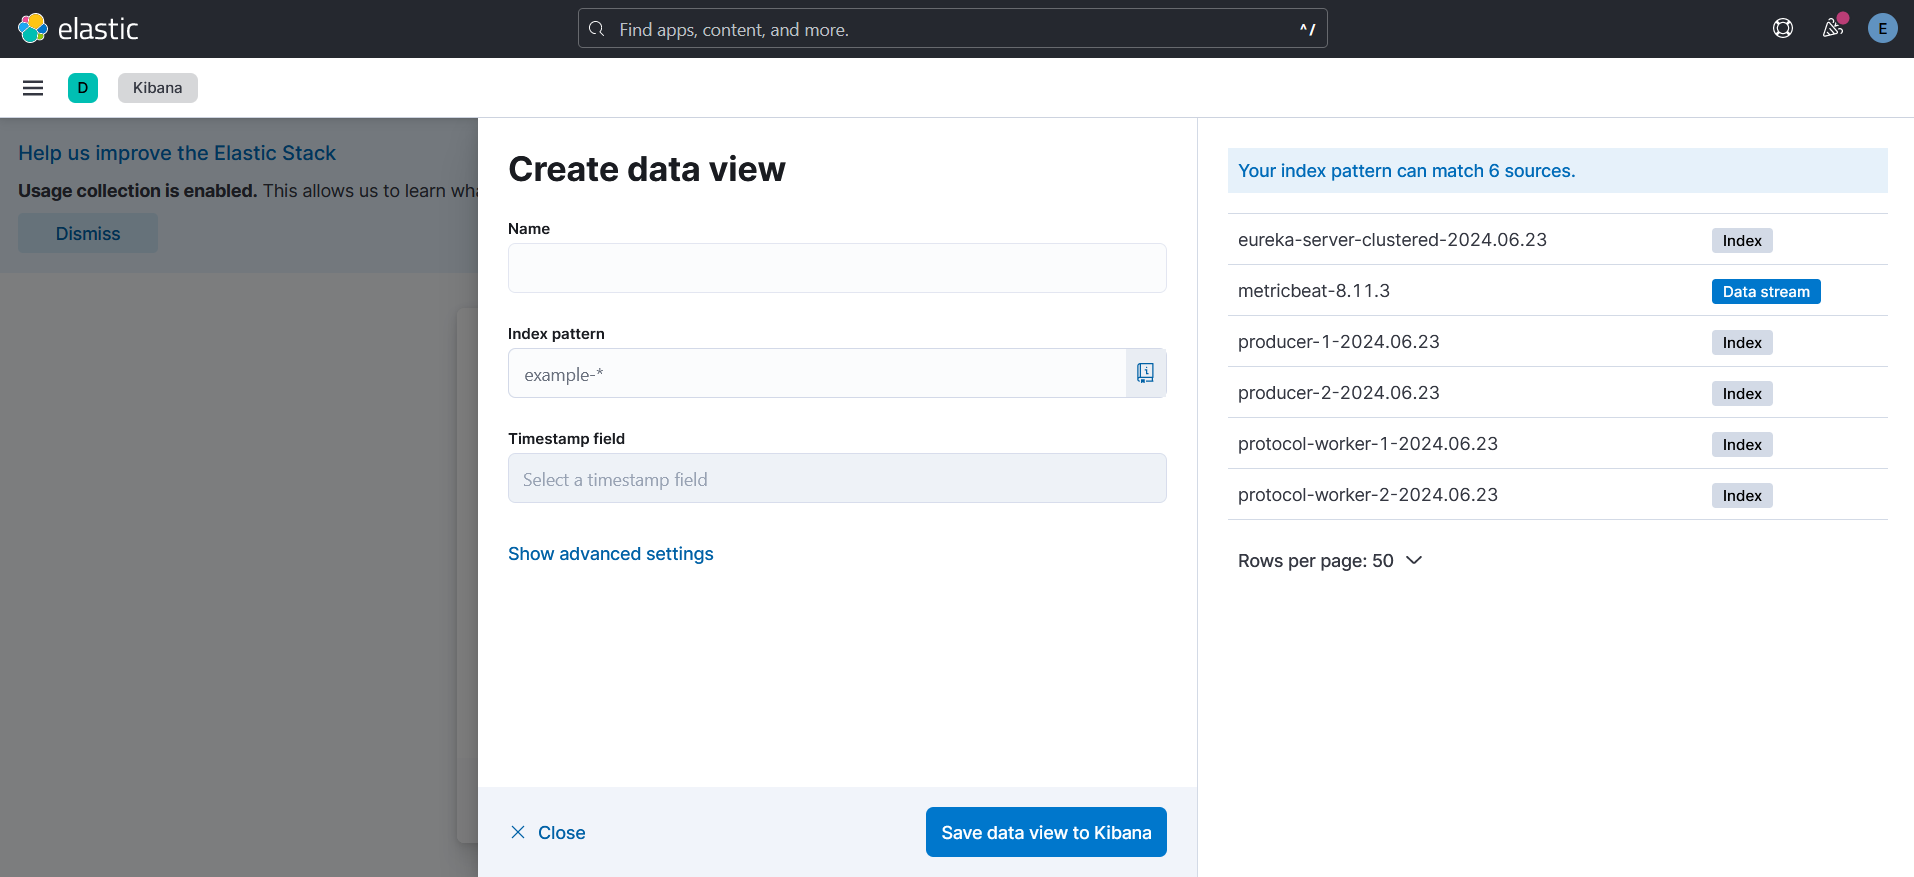
\includegraphics[width=\textwidth]{images/implementation/kibanaDiscoveryDataView.png}
    \caption{Kibana --- przechwycone dzienniki zdarzeń}
    \label{kibanaDiscoveryDataView}
\end{figure}

\subsection{Monitorowanie podsystemu}

Blok "Monitorowanie podsystemu" odbywa się za pośrednictwem usługi Metricbeat, która zbiera i wysyła metryki z różnych systemów i usług. Metricbeat gromadzi metryki na poziomie systemu, takie jak użycie procesora, użycie pamięci, dysku i ruchu sieciowego, następnie wysyła te dane do Elasticsearch. Dane te są następnie analizowane i wizualizowane w usłudze Kibana, zapewniając kompleksowe monitorowanie wydajności infrastruktury, kondycji i wykorzystania zasobów.

\section{Uruchomienie środowiska}

\subsection{Bazowe środowisko}

W celu uruchomienia systemu, na komputerze wymagane są zainstalowane narzędzia \verb|Docker| i \verb|Docker Compose|. Głównym plikiem niezbędnym to uruchomienia systemu jest plik docker-compose.yml zaprezentowany w dodatku \ref{dockerComposeRef}, w którym zdefiniowane są usługi monitoringu systemu oraz rozproszony rejestr usług.

Bloki x--common--elastisearch--image (linie 3-4), x-common--logstash--image (linie 5-6) i x--common--my--eureka--image (linie 7-9) definiują informacje o konfiguracji wielokrotnego użytku odpowiednio dla Elasticsearch, Logstash i obrazu rejestru usług. Są one wykorzystywane w celu uniknięcia powtórzeń definicji obrazu w poszczególnych usługach.

Sekcja woluminów (linie 11-29) definiuje trwałe obszary przechowywania dla poszczególnych kontenerów.

Sekcja sieci (linie 31-37), definiuje sieć razem z podsiecią łączącą usługi w ramach uruchamianego środowiska.

Podstawowe środowisko składa się z następujących usług:
\begin{itemize}
    \item Usługa \verb|setup| (linie 40-109) generuje certyfikaty Elasticsearch. 
    \item Zdefiniowane są trzy węzły Elasticsearch o nazwach \verb|elasticsearch01|, \verb|elasticsearch02| i \verb|elasticsearch01| (linie 111-262). Są one zależne od usługi \verb|setup|. Każda z tych usług przyjmuje w polu \verb|discovery.seed_hosts| adresy pozostałych uruchomionych usług Elasticsearch w celu utworzenia klastra usług zapewniającego wysoką dostępność.
    \item Usługa \verb|Kibana| (linie 264-305) łączy się z klastrem Elasticsearch w celu dostępu do zbieranych dokumentów i wizualizacji danych w interfejsie sieciowym uruchomionym na porcie 5601.
    \item Trzy instancje Logstash o nazwach logstash01, logstash02 i logstash03 (linie 307-452) są zdefiniowane do obsługi pozyskiwania i przetwarzania danych. Każda instancja Logstash przyjmuje łączy się z każdym węzłem z uruchomionego klastra Elasticsearch w celu zapewnienia wysokiej dostępności w razie awarii węzłów w klastrze.
    \item Usługa \verb|metricbeat01| (linie 454-489) służy do zbierania metryk z innych usług ze stosu \akronim{ELK} i wysyłania tych metryk do klastra Elasticsearch.
    \item Trzy instancje serwera Eureka o nazwach eureka--server--peer--1, eureka--server--peer--2 i eureka--server--peer--3 (linie 491-576) są zdefiniowane do wykrywania usług w systemie. Do każdej usługi są podane zmienne środowiskowo uruchamiające usługę jako wcześniej zdefiniowany profil aplikacyjny w celu uruchomienia klastra rejestrów Eureka.
\end{itemize}

Aby uruchomić powyższą konfigurację Docker Compose, w głównym folderze projektu należy użyć następującego polecenia:

\begin{verbatim}
sudo docker compose --env-file ELK-monitoring/.env down -v && \
sudo docker compose --env-file ELK-monitoring/.env build --no-cache && \
sudo docker compose --env-file ELK-monitoring/.env up --force-recreate -d
\end{verbatim}

Powyższe polecenie wykonuje następujące czynności:

\begin{itemize}
    \item Zatrzymuje i usuwa wszystkie uruchomione usługi i woluminy.
    \item Buduje obrazy Docker bez użycia pamięci podręcznej.
    \item Uruchamia usługi, wymuszając odtworzenie kontenerów i uruchomienie ich w trybie odłączonym.
\end{itemize}

Opisany plik \verb|docker-compose.yml| konfiguruje środowisko rozruchowe klastra Elasticsearch, wraz z instancjami Logstash do przetwarzania danych, Kibana do wizualizacji, Metricbeat do zbierania metryk i konfiguracją serwera Eureka do wykrywania usług w systemie. Usługi są połączone za pomocą sieci Docker, a trwałe przechowywanie w przypadku wyłączenia systemu jest zarządzane za pomocą woluminów Docker. Wykorzystanie zmiennych środowiskowych i kontroli stanu kontenerów zapewnia, że usługi są poprawnie skonfigurowane i uruchamiane w ściśle określonej kolejności.

\subsection{Producent}

Skrypt Bash przedstawiony na listingu.\ref{producerBashScript} jest przeznaczony do uruchamiania wielu instancji usługi kontenerowej Docker, z których każda reprezentuje producenta. Skrypt zapewnia dostępność obrazu Docker dla producentów, buduje go w razie potrzeby, a następnie uruchamia określoną liczbę instancji producentów z odpowiednimi zmiennymi środowiskowymi i konfiguracjami sieciowymi.

\begin{lstlisting}[language=bash,caption=Kod skryptu producers.sh,label=producerBashScript]
    #!/bin/bash

    # Check if the necessary arguments are provided
    if [ $# -ne 2 ]; then
        echo "Usage: $0 <first producer id> <number of producers>"
        exit 1
    fi
    
    # First producer ID and number of producers to run
    first_producer_id=$1
    num_producers=$2
    
    # Function to check if the Docker image exists and build it if not
    ensure_docker_image() {
        if [ -z "$(docker images -q producer:latest 2> /dev/null)" ]; then
            echo "'producer:latest' image not found. Building image..."
            if ! docker build Producer -t producer:latest --no-cache; then
                echo "Error building Docker image 'producer:latest'. Exiting."
                exit 1
            fi
        fi
    }
    
    # Ensure the Docker image is available
    ensure_docker_image
    
    # Loop and run the Docker command
    for (( i=first_producer_id; i<first_producer_id+num_producers; i++ )); do
    
        docker run --rm -d --network=masterNetwork \
        -e PEER_1_URL=http://172.20.0.2:9001/eureka/,http://172.20.0.3:9002/eureka/,http://172.20.0.4:9003/eureka/ \
        -e PRODUCER_ID=$i \
        -e LOGSTASH_DESTINATION_ONE=172.20.0.12:5000 \
        -e LOGSTASH_DESTINATION_TWO=172.20.0.13:5000 \
        -e LOGSTASH_DESTINATION_THREE=172.20.0.14:5000 \
        -e NUMBER_OF_PRODUCTS=10 \
        -e PORT=10000 \
        -p $((10000+$i)):10000 \
        --name=PRODUCER_$i producer:latest
    
    done

\end{lstlisting}

Skrypt oczekuje dwóch argumentów: identyfikatora pierwszego producenta (linia 10) i liczby instancji producenta do uruchomienia (linia 11). Jeżeli te argumenty nie zostaną dostarczone, skrypt wyświetli informacje o braku argumentów i zakończy działanie. Następnie funkcja ensure\_docker\_image (linie 14-22) sprawdza, czy obraz Docker o nazwie \verb|producer:latest| istnieje. Jeśli obraz nie istnieje, buduje obraz z katalogu Producer. Jeśli kompilacja nie powiedzie się, skrypt kończy działanie z komunikatem o błędzie. Następnie skrypt wykonuje pętlę (linie 28-39) od pierwszego identyfikatora producenta do określonej liczby producentów. Dla każdej iteracji uruchamia kontener Docker z niezbędnymi zmiennymi środowiskowymi i konfiguracjami sieciowymi. Każdy kontener ma unikalną nazwę i jest połączony z siecią \verb|masterNetwork|.

Skrypt \verb|producers.sh| automatyzuje wdrażanie wielu instancji producentów. Zapewnia on dostępność wymaganego obrazu Docker, buduje go w razie potrzeby, a następnie uruchamia określoną liczbę producentów z odpowiednimi konfiguracjami. Ta konfiguracja jest przydatna do testowania i skalowania usług producentów w kontrolowanym środowisku.

\subsection{Węzeł protokołu}

Skrypt przedstawiony na listingu.\ref{workersBashScript} jest przeznaczony do uruchamiania wielu instancji aplikacji kontenerowej Docker, z których każda reprezentuje węzeł protokołu. Skrypt zapewnia dostępność obrazu Docker dla węzła protokołu, buduje go w razie potrzeby, a następnie uruchamia określoną liczbę instancji węzłów z odpowiednimi zmiennymi środowiskowymi i konfiguracjami sieciowymi.

\begin{lstlisting}[language=bash,caption=Kod skryptu workers.sh,label=workersBashScript]
    #!/bin/bash

    # Check if the necessary arguments are provided
    if [ $# -ne 2 ]; then
        echo "Usage: $0 <first worker id> <number of workers>"
        exit 1
    fi
    
    # First producer ID and number of producers to run
    first_worker_id=$1
    num_workers=$2
    
    # Function to check if the Docker image exists and build it if not
    ensure_docker_image() {
        if [ -z "$(docker images -q worker:latest 2> /dev/null)" ]; then
            echo "'worker:latest' image not found. Building image..."
            if ! docker build Master-Protocol-Worker -t worker:latest --no-cache; then
                echo "Error building Docker image 'worker:latest'. Exiting."
                exit 1
            fi
        fi
    }
    
    # Ensure the Docker image is available
    ensure_docker_image
    
    # Loop and run the Docker command
    for (( i=first_worker_id; i<first_worker_id+num_workers; i++ )); do
    
        docker run --rm -d --network=masterNetwork \
        -e PEER_1_URL=http://172.20.0.2:9001/eureka/,http://172.20.0.3:9002/eureka/,http://172.20.0.4:9003/eureka/ \
        -e WORKER_ID=$i \
        -e LOGSTASH_DESTINATION_ONE=172.20.0.12:5000 \
        -e LOGSTASH_DESTINATION_TWO=172.20.0.13:5000 \
        -e LOGSTASH_DESTINATION_THREE=172.20.0.14:5000 \
        -e PORT=11000\
        -p $((12000+$i)):11000 \
        --name=Worker-$i \
        worker
    
    done
\end{lstlisting}

Skrypt oczekuje dwóch argumentów: identyfikatora pierwszego węzła (linia 10) i liczby instancji węzłów do uruchomienia (linia 11). Jeżeli te argumenty nie zostaną dostarczone, skrypt wyświetli informacje o braku argumentów i zakończy działanie. Funkcja ensure\_docker\_image (linie 14-22) sprawdza, czy obraz Docker o nazwie \verb|worker:latest| istnieje. Jeżeli obraz nie istnieje, buduje obraz z katalogu Master--Protocol--Worker. Jeśli kompilacja nie powiedzie się, skrypt kończy działanie z komunikatem o błędzie. Następnie skrypt wykonuje pętlę (linie 28-39) od pierwszego identyfikatora węzła do określonej liczby węzłów. Dla każdej iteracji uruchamia kontener Docker z niezbędnymi zmiennymi środowiskowymi i konfiguracjami sieciowymi. Każdy kontener ma unikalną nazwę i jest połączony z siecią \verb|masterNetwork|.

Skrypt automatyzuje wdrażanie wielu instancji roboczych w sieci Docker. Zapewnia on dostępność wymaganego obrazu Docker, buduje go w razie potrzeby, a następnie uruchamia określoną liczbę pracowników z odpowiednimi konfiguracjami. Ta konfiguracja jest przydatna do testowania i skalowania usług roboczych w kontrolowanym środowisku.

\chapter{Testy Systemu}

\section{Przeprowadzane testy}

W celu weryfikacji działania zaproponowanego systemu, przeprowadzono testy wydajnościowe, aby ocenić, w jaki sposób system obsługuje liczne żądania wykonywane równolegle oraz szeregowo. Testy te miały na celu zweryfikowanie zachowania systemu podczas ogólnego użytkowania. Testy zostały wykonane poprzez uruchomienie skryptów powłoki jednocześnie w wielu lokalizacjach.

\section{Platforma testowa}

Testowany system przedstawiony na rys.\ref{testowySystemSchemat} został uruchomiony na jednej fizycznej maszynie podłączonej do sieci lokalnej poprzez kabel ethernet, podczas gdy dodatkowy węzeł protokołu był uruchomiony na Raspberry Pi zero 2W podłączonej do sieci lokalnej poprzez WIFI. Główną testową wartością był czas obsługi żądania.

Parametry platformy testowej to:

\begin{itemize}
    \item Procesor \akronim{CPU} (\english{Central Processing Unit}) - Intel(R) Core(TM) i7-9750H CPU @ 2.60GHz
    \item Dysk twardy - Samsung SSD 980 PRO 1TB
    \item Pamięć \akronim{RAM} (\english{Random-Access Memory}) - Kingston Fury Impact 16GB [1x16GB 2666MHz DDR4 CL15 SODIMM] + Kingston 8 GB DDR4 2666 MHz
\end{itemize}


\begin{figure}
    \centering
    \includesvg[width=\textwidth]{schemas/tests/testEnvironment.svg}
    \caption{Schemat testowego środowiska}
    \label{testowySystemSchemat}
\end{figure}

Na rys.\ref{testraspberryPiGraph} przedstawiony został wykres przedstawiający czasy odpowiedzi dla 1000 żądań wykonanych przez Raspberry Pi Zero 2W podłączone przez Wi-Fi do sieci. Wartości wykazują znaczną zmienność, z niektórymi czasami odpowiedzi sięgającymi około 800 milisekund, dłuższy czas przetwarzania pierwszej wiadomości jest spowodowany ustawianiem w systemie wartości niezbędnych do określania ścieżek w sieci \akronim{LAN} (\english{Local Area Network}). Średni czas odpowiedzi wynosi 156,19 milisekund, co jest przedstawione na wykresie czerwoną przerywaną linią.

\begin{figure}
    \centering
    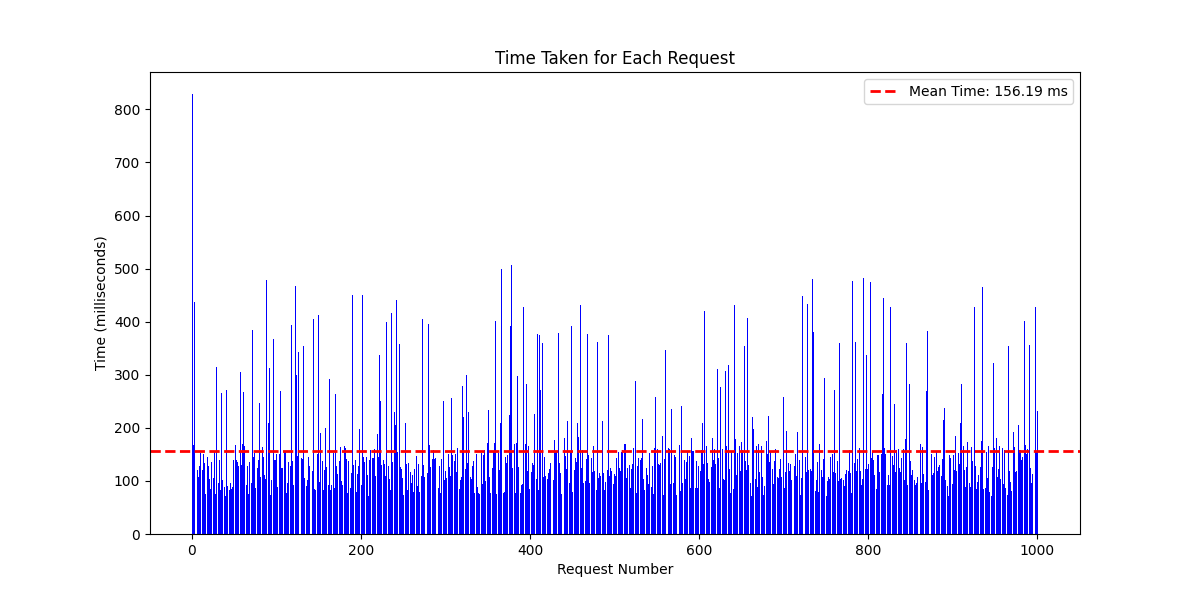
\includegraphics[width=\textwidth]{images/testy/tests.png}
    \caption{Wykres czasu obsługi żądań wysłanych z raspberry pi zero 2W}
    \label{testraspberryPiGraph}
\end{figure}

 Na rys.\ref{testlocalhostGraph} przedstawiony został wykres ilustrujący czasy odpowiedzi dla 1000 żądań wykonanych do platformy testowej (ten sam komputer z uruchomionym systemem). W porównaniu do poprzedniego wykresu, czasy odpowiedzi są zdecydowanie niższe i bardziej spójne, z większością wartości poniżej 100 milisekund. Średni czas odpowiedzi wynosi 64,29 milisekundy, czyli znacznie mniej niż w przypadku uruchomienia testu na Raspberry Pi. Wykres ten pokazuje lepszą wydajność i mniejsze opóźnienia, gdy żądania są wykonywane na tym samym komputerze, omijając opóźnienia związane z siecią.


\begin{figure}[!htbp]
    \centering
    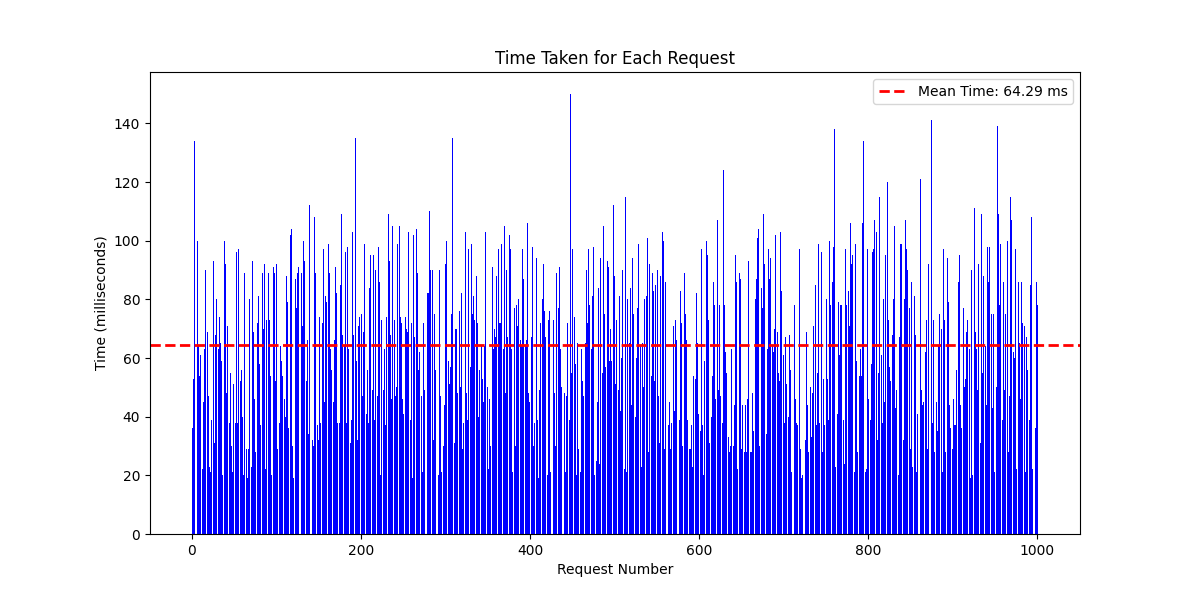
\includegraphics[width=\textwidth]{images/testy/testsLocalhost.png}
    \caption{Wykres czasu obsługi żądań z wysłanych z platformy testowej}
    \label{testlocalhostGraph}
\end{figure}

Wykonane testy przedstawiają wyraźne porównanie różnic w wydajności w systemie rozproszonym przy wykorzystaniu Wi-Fi oraz aplikacji uruchomionej na tym samym urządzeniu co system, podkreślając wpływ komunikacji sieciowej na czasy odpowiedzi w systemie.

\chapter{Podsumowanie}

Celem pracy było stworzenie systemu  pozwalającego na zarządzanie zasobami w środowisku Metaverse. System składa się z systemu zarządzania zasobami oraz systemu monitorowania usług znajdujących się w systemie. Udało się zrealizować całość zaplanowanych prac. W wyniku przeprowadzonych prac powstały trzy usługi w systemie zarządzania zasobami:rozproszony rejestr usług Eureka, węzeł protokołu oraz usługa producenta świadcząca usługi w systemie. System zarządzania zasobami, koordynuje wielu producentów i węzłów protokołu. Obejmuje on mechanizm wykrywania usług, zapewniający interakcję między różnymi komponentami systemu. Węzły protokołu obsługują żądania od użytkowników, podczas gdy producenci świadczą usługi oraz zasoby udostępniane w środowisku Metaverse. Rejestr Eureka zapewnia wysoką dostępność i równoważenie obciążenia w różnych węzłach, zwiększając tym samym niezawodność i wydajność systemu. Podsystem monitoringu, integruje narzędzia takie jak Elasticsearch, Logstash oraz Kibana zapewniając kompleksowy monitoring wszystkich usług uruchomionych w systemie. Podsystem monitoringu przechwytuje, przechowuje i wizualizuje dane dotyczące usług producenta, węzła protokołu i rejestru Eureka. 

Zaimplementowany system spełnia wszystkie wcześniej określone założenia i wymagania, zapewniając niezbędne funkcjonalności do zarządzania środowiskiem Metaverse. Wybory projektowe i wdrożeniowe, takie jak mechanizm wykrywania usług i konteneryzacja systemu oraz wykorzystanie Elasticsearch do monitorowania, zapewniają wydajność, niezawodność i skalowalność systemu.

Niniejsza rozprawa demonstruje praktyczne zastosowanie systemów rozproszonych i chmurowych w rozwijającej się dziedzinie Metaverse, pokazując, w jaki sposób architektura modułowa i nowoczesne praktyki inżynierii oprogramowania mogą tworzyć elastyczne i wydajne rozwiązania do zarządzania zasobami.

Na podstawie projektu systemu oraz analizy koncepcyjnych rozwiązań i na podstawie istniejących narzędzi został zaimplementowany system zapewniający funkcjonalność zarządzania zasobami w środowisku Metaverse. Istnieją jednak dodatkowe funkcjonalności, których brak nie ogranicza działania systemu, jednak mogą one znacząco poszerzyć jego możliwości. Jedną z pierwszych funkcji dodanych do nowej wersji systemu będzie wdrożenie algorytmów uczenia maszynowego do analizy predykcyjnej. Pozwoli to systemowi prognozować przyszłe zapotrzebowanie na zasoby w oparciu o dane historyczne i wzorce użytkowania, optymalizując alokację zasobów i zmniejszając koszty operacyjne. Dodatkowo wprowadzone zostanie wykrywanie anomalii za pomocą modeli uczenia maszynowego. Umożliwi to systemowi identyfikację nietypowych wzorców lub anomalii w funkcjonowaniu systemu, które mogą wskazywać na potencjalne zagrożenia bezpieczeństwa lub awarie systemu. Następną funkcją będzie wprowadzenie systemu rekomendacji. System ten będzie sugerował użytkownikom odpowiednie zasoby lub treści w oparciu o ich preferencje i zachowanie w Metaverse, zwiększając komfort użytkowania. Kolejną funkcjonalnością będzie monitorowanie oparte na sztucznej inteligencji, które będzie analizować dane zapewniając proaktywne zalecenia dotyczące optymalizacji wydajności i niezawodności systemu.

wprowadzenie zaproponowanej funkcjonalności pozwoli, by system ewoluował, aby stać się bardziej inteligentnym, bezpiecznym i zorientowanym na użytkownika, skutecznie zaspokajając dynamiczne potrzeby środowiska Metaverse.

%--------------------------------------
% Literatura
%--------------------------------------

\bibliographystyle{IEEEtran}{\raggedright\sloppy\small\bibliography{bibliografia}}

%--------------------------------------
% Spis ilustracji
%--------------------------------------
\newpage
\listoffigures

%--------------------------------------
% Spis listingów
%--------------------------------------
\newpage
\lstlistoflistings

%--------------------------------------
% Dodatki
%--------------------------------------

\cleardoublepage\appendix%
\chapter{Plik Docker-Compose.yml}
\label{dockerComposeRef}
\begin{lstlisting}[caption=Plik docker-comose.yml, label=dockerComposeFile]
    version: '3.8'
    
    x-common-elastisearch-image: &elasticsearchImage
      image: docker.elastic.co/elasticsearch/elasticsearch:${STACK_VERSION}
    x-common-logstash-image: &logstashImage
      image: docker.elastic.co/logstash/logstash:${STACK_VERSION}
    x-common-my-eureka-image: &myEureka
      build: Service-registry
      image: my-eureka-builder-image
    
    volumes:
      certs:
        driver: local
      esdata01:
        driver: local
      esdata02:
        driver: local
      esdata03:
        driver: local
      kibanadata:
        driver: local
      metricbeatdata01:
        driver: local
      logstashdata01:
        driver: local
      logstashdata02:
        driver: local
      logstashdata03:
        driver: local
    
    networks:
      masterNetwork:
        driver: bridge
        name: masterNetwork
        ipam:
          config:
            - subnet: 172.20.0.0/16
    
    services:  
      setup:
        container_name: setup
        <<: *elasticsearchImage
        volumes:
          - certs:/usr/share/elasticsearch/config/certs
        user: "0"
        networks:
          masterNetwork:
            ipv4_address: 172.20.0.5
        command: >
          bash -c '
            if [ x${ELASTIC_PASSWORD} == x ]; then
              echo "Set the ELASTIC_PASSWORD environment variable in the .env file";
              exit 1;
            elif [ x${KIBANA_PASSWORD} == x ]; then
              echo "Set the KIBANA_PASSWORD environment variable in the .env file";
              exit 1;
            fi;
            if [ ! -f config/certs/ca.zip ]; then
              echo "Creating CA";
              bin/elasticsearch-certutil ca --silent --pem -out config/certs/ca.zip;
              unzip config/certs/ca.zip -d config/certs;
            fi;
            if [ ! -f config/certs/certs.zip ]; then
              echo "Creating certs";
              echo -ne \
              "instances:\n"\
              "  - name: es01\n"\
              "    dns:\n"\
              "      - es01\n"\
              "      - localhost\n"\
              "    ip:\n"\
              "      - 127.0.0.1\n"\
              "  - name: es02\n"\
              "    dns:\n"\
              "      - es02\n"\
              "      - localhost\n"\
              "    ip:\n"\
              "      - 127.0.0.1\n"\
              "  - name: es03\n"\
              "    dns:\n"\
              "      - es03\n"\
              "      - localhost\n"\
              "    ip:\n"\
              "      - 127.0.0.1\n"\
              "  - name: kibana\n"\
              "    dns:\n"\
              "      - kibana\n"\
              "      - localhost\n"\
              "    ip:\n"\
              "      - 127.0.0.1\n"\
              > config/certs/instances.yml;
              bin/elasticsearch-certutil cert --silent --pem -out config/certs/certs.zip --in config/certs/instances.yml --ca-cert config/certs/ca/ca.crt --ca-key config/certs/ca/ca.key;
              unzip config/certs/certs.zip -d config/certs;
            fi;
            echo "Setting file permissions"
            chown -R root:root config/certs;
            find . -type d -exec chmod 750 \{\} \;;
            find . -type f -exec chmod 640 \{\} \;;
            echo "Waiting for Elasticsearch availability";
            until curl -s --cacert config/certs/ca/ca.crt https://es01:9200 | grep -q "missing authentication credentials"; do sleep 30; done;
            echo "Setting kibana_system password";
            until curl -s -X POST --cacert config/certs/ca/ca.crt -u "elastic:${ELASTIC_PASSWORD}" -H "Content-Type: application/json" https://es01:9200/_security/user/kibana_system/_password -d "{\"password\":\"${KIBANA_PASSWORD}\"}" | grep -q "^{}"; do sleep 10; done;
            echo "All done!";
          '
        healthcheck:
          test: ["CMD-SHELL", "[ -f config/certs/es01/es01.crt ]"]
          interval: 1s
          timeout: 5s
          retries: 120
    
      es01:
        container_name: elasticsearch01
        depends_on:
          setup:
            condition: service_healthy
        <<: *elasticsearchImage
        volumes:
          - certs:/usr/share/elasticsearch/config/certs
          - esdata01:/usr/share/elasticsearch/data
        ports:
          - ${ES_PORT}:9200
        networks:
          masterNetwork:
            ipv4_address: 172.20.0.6
        environment:
          - node.name=es01
          - cluster.name=${CLUSTER_NAME}
          - cluster.initial_master_nodes=es01,es02,es03
          - discovery.seed_hosts=es02,es03
          - ELASTIC_PASSWORD=${ELASTIC_PASSWORD}
          - bootstrap.memory_lock=true
          - xpack.security.enabled=true
          - xpack.security.http.ssl.enabled=true
          - xpack.security.http.ssl.key=certs/es01/es01.key
          - xpack.security.http.ssl.certificate=certs/es01/es01.crt
          - xpack.security.http.ssl.certificate_authorities=certs/ca/ca.crt
          - xpack.security.transport.ssl.enabled=true
          - xpack.security.transport.ssl.key=certs/es01/es01.key
          - xpack.security.transport.ssl.certificate=certs/es01/es01.crt
          - xpack.security.transport.ssl.certificate_authorities=certs/ca/ca.crt
          - xpack.security.transport.ssl.verification_mode=certificate
          - xpack.license.self_generated.type=${LICENSE}
          - xpack.monitoring.collection.enabled=true
        mem_limit: 1g
        deploy:
          resources:
            limits:
              cpus: '0.5'
              memory: 1g
        ulimits:
          memlock:
            soft: -1
            hard: -1
        healthcheck:
          test:
            [
              "CMD-SHELL",
              "curl -s --cacert config/certs/ca/ca.crt https://localhost:9200 | grep -q 'missing authentication credentials'",
            ]
          interval: 10s
          timeout: 10s
          retries: 120
    
      es02:
        container_name: elasticsearch02
        depends_on:
          - es01
        <<: *elasticsearchImage
        networks:
          masterNetwork:
            ipv4_address: 172.20.0.7
        volumes:
          - certs:/usr/share/elasticsearch/config/certs
          - esdata02:/usr/share/elasticsearch/data
        environment:
          - node.name=es02
          - cluster.name=${CLUSTER_NAME}
          - cluster.initial_master_nodes=es01,es02,es03
          - discovery.seed_hosts=es01,es03
          - ELASTIC_PASSWORD=${ELASTIC_PASSWORD}
          - bootstrap.memory_lock=true
          - xpack.security.enabled=true
          - xpack.security.http.ssl.enabled=true
          - xpack.security.http.ssl.key=certs/es02/es02.key
          - xpack.security.http.ssl.certificate=certs/es02/es02.crt
          - xpack.security.http.ssl.certificate_authorities=certs/ca/ca.crt
          - xpack.security.transport.ssl.enabled=true
          - xpack.security.transport.ssl.key=certs/es02/es02.key
          - xpack.security.transport.ssl.certificate=certs/es02/es02.crt
          - xpack.security.transport.ssl.certificate_authorities=certs/ca/ca.crt
          - xpack.security.transport.ssl.verification_mode=certificate
          - xpack.license.self_generated.type=${LICENSE}
          - xpack.monitoring.collection.enabled=true
        mem_limit: 1g
        deploy:
          resources:
            limits:
              cpus: '0.5'
              memory: 1g
        ulimits:
          memlock:
            soft: -1
            hard: -1
        healthcheck:
          test:
            [
              "CMD-SHELL",
              "curl -s --cacert config/certs/ca/ca.crt https://localhost:9200 | grep -q 'missing authentication credentials'",
            ]
          interval: 10s
          timeout: 10s
          retries: 120
    
      es03:
        container_name: elasticsearch03
        depends_on:
          - es02
        <<: *elasticsearchImage
        networks:
          masterNetwork:
            ipv4_address: 172.20.0.8
        volumes:
          - certs:/usr/share/elasticsearch/config/certs
          - esdata03:/usr/share/elasticsearch/data
        environment:
          - node.name=es03
          - cluster.name=${CLUSTER_NAME}
          - cluster.initial_master_nodes=es01,es02,es03
          - discovery.seed_hosts=es01,es02
          - ELASTIC_PASSWORD=${ELASTIC_PASSWORD}
          - bootstrap.memory_lock=true
          - xpack.security.enabled=true
          - xpack.security.http.ssl.enabled=true
          - xpack.security.http.ssl.key=certs/es03/es03.key
          - xpack.security.http.ssl.certificate=certs/es03/es03.crt
          - xpack.security.http.ssl.certificate_authorities=certs/ca/ca.crt
          - xpack.security.transport.ssl.enabled=true
          - xpack.security.transport.ssl.key=certs/es03/es03.key
          - xpack.security.transport.ssl.certificate=certs/es03/es03.crt
          - xpack.security.transport.ssl.certificate_authorities=certs/ca/ca.crt
          - xpack.security.transport.ssl.verification_mode=certificate
          - xpack.license.self_generated.type=${LICENSE}
          - xpack.monitoring.collection.enabled=true
        mem_limit: 1g
        deploy:
          resources:
            limits:
              cpus: '0.5'
              memory: 1g
        ulimits:
          memlock:
            soft: -1
            hard: -1
        healthcheck:
          test:
            [
              "CMD-SHELL",
              "curl -s --cacert config/certs/ca/ca.crt https://localhost:9200 | grep -q 'missing authentication credentials'",
            ]
          interval: 10s
          timeout: 10s
          retries: 120
    
      kibana:
        container_name: kibana
        depends_on:
          es01:
            condition: service_healthy
          es02:
            condition: service_healthy
          es03:
            condition: service_healthy
        image: docker.elastic.co/kibana/kibana:${STACK_VERSION}
        volumes:
          - certs:/usr/share/kibana/config/certs
          - kibanadata:/usr/share/kibana/data
        ports:
          - ${KIBANA_PORT}:5601
        networks:
          masterNetwork:
            ipv4_address: 172.20.0.9
        environment:
          - SERVERNAME=kibana
          - ELASTICSEARCH_HOSTS=["https://es01:9200","https://es02:9200","https://es03:9200"]
          - ELASTICSEARCH_USERNAME=kibana_system
          - ELASTICSEARCH_PASSWORD=${KIBANA_PASSWORD}
          - ELASTICSEARCH_SSL_CERTIFICATEAUTHORITIES=config/certs/ca/ca.crt
          - XPACK_SECURITY_ENCRYPTIONKEY=${ENCRYPTION_KEY}
          - XPACK_ENCRYPTEDSAVEDOBJECTS_ENCRYPTIONKEY=${ENCRYPTION_KEY}
          - XPACK_REPORTING_ENCRYPTIONKEY=${ENCRYPTION_KEY}
        mem_limit: 1g
        deploy:
          resources:
            limits:
              cpus: '0.5'
              memory: 1g
        healthcheck:
          test:
            [
              "CMD-SHELL",
              "curl -s -I http://localhost:5601 | grep -q 'HTTP/1.1 302 Found'",
            ]
          interval: 10s
          timeout: 10s
          retries: 120
    
      logstash01:
        <<: *logstashImage
        container_name: logstash01
        ports:
          - 5000:5000
        depends_on:
          es01:
            condition: service_healthy
          es02:
            condition: service_healthy
          es03:
            condition: service_healthy
          kibana:
            condition: service_healthy
        labels:
          co.elastic.logs/module: logstash
        user: root
        networks:
          masterNetwork:
            ipv4_address: 172.20.0.12
        volumes:
          - certs:/usr/share/logstash/certs
          - logstashdata01:/usr/share/logstash/data
          - "./ELK-monitoring/logstash_ingest_data/:/usr/share/logstash/ingest_data/"
          - "./ELK-monitoring/logstashConfig/pipeline:/usr/share/logstash/pipeline:ro"
        environment:
          - xpack.monitoring.enabled=true
          - xpack.monitoring.collection.enabled=true
          - xpack.monitoring.elasticsearch.hosts=["https://es01:9200","https://es02:9200","https://es03:9200"]
          - xpack.monitoring.elasticsearch.username="elastic"
          - xpack.monitoring.elasticsearch.password=${ELASTIC_PASSWORD}
          - xpack.monitoring.elasticsearch.ssl.certificate_authority=certs/ca/ca.crt
          - ELASTIC_USER=elastic
          - ELASTIC_PASSWORD=${ELASTIC_PASSWORD}
        mem_limit: 512m
        deploy:
          resources:
            limits:
              cpus: '0.25'
              memory: 512m
        healthcheck:
          test: [
            "CMD-SHELL",
            "curl -XGET 'localhost:9600/_node/stats'"
          ]
          interval: 30s
          timeout: 10s
          retries: 120
    
      logstash02:
        <<: *logstashImage
        container_name: logstash02
        ports:
          - 5001:5000
        depends_on:
          es01:
            condition: service_healthy
          es02:
            condition: service_healthy
          es03:
            condition: service_healthy
          kibana:
            condition: service_healthy
        labels:
          co.elastic.logs/module: logstash
        user: root
        networks:
          masterNetwork:
            ipv4_address: 172.20.0.13
        volumes:
          - certs:/usr/share/logstash/certs
          - logstashdata02:/usr/share/logstash/data
          - "./ELK-monitoring/logstash_ingest_data/:/usr/share/logstash/ingest_data/"
          - "./ELK-monitoring/logstashConfig/pipeline:/usr/share/logstash/pipeline:ro"
        environment:
          - xpack.monitoring.enabled=true
          - xpack.monitoring.collection.enabled=true
          - xpack.monitoring.elasticsearch.hosts=["https://es01:9200","https://es02:9200","https://es03:9200"]
          - xpack.monitoring.elasticsearch.username="elastic"
          - xpack.monitoring.elasticsearch.password=${ELASTIC_PASSWORD}
          - xpack.monitoring.elasticsearch.ssl.certificate_authority=certs/ca/ca.crt
          - ELASTIC_USER=elastic
          - ELASTIC_PASSWORD=${ELASTIC_PASSWORD}
        mem_limit: 512m
        deploy:
          resources:
            limits:
              cpus: '0.25'
              memory: 512m
        healthcheck:
          test: [
            "CMD-SHELL",
            "curl -XGET 'localhost:9600/_node/stats'"
          ]
          interval: 30s
          timeout: 10s
          retries: 120
    
      logstash03:
        <<: *logstashImage
        container_name: logstash03
        ports:
          - 5002:5000
        depends_on:
          es01:
            condition: service_healthy
          es02:
            condition: service_healthy
          es03:
            condition: service_healthy
          kibana:
            condition: service_healthy
        labels:
          co.elastic.logs/module: logstash
        user: root
        networks:
          masterNetwork:
            ipv4_address: 172.20.0.14
        volumes:
          - certs:/usr/share/logstash/certs
          - logstashdata03:/usr/share/logstash/data
          - "./ELK-monitoring/logstash_ingest_data/:/usr/share/logstash/ingest_data/"
          - "./ELK-monitoring/logstashConfig/pipeline:/usr/share/logstash/pipeline:ro"
        environment:
          - xpack.monitoring.enabled=true
          - xpack.monitoring.collection.enabled=true
          - xpack.monitoring.elasticsearch.hosts=["https://es01:9200","https://es02:9200","https://es03:9200"]
          - xpack.monitoring.elasticsearch.username="elastic"
          - xpack.monitoring.elasticsearch.password=${ELASTIC_PASSWORD}
          - xpack.monitoring.elasticsearch.ssl.certificate_authority=certs/ca/ca.crt
          - ELASTIC_USER=elastic
          - ELASTIC_PASSWORD=${ELASTIC_PASSWORD}
        mem_limit: 512m
        deploy:
          resources:
            limits:
              cpus: '0.25'
              memory: 512m
        healthcheck:
          test: [
            "CMD-SHELL",
            "curl -XGET 'localhost:9600/_node/stats'"
          ]
          interval: 30s
          timeout: 10s
          retries: 120
    
      metricbeat01:
        container_name: metricbeat01
        depends_on:
          es01:
            condition: service_healthy
          es02:
            condition: service_healthy
          es03:
            condition: service_healthy
          kibana:
            condition: service_healthy
        image: docker.elastic.co/beats/metricbeat:${STACK_VERSION}
        user: root
        networks:
          masterNetwork:
            ipv4_address: 172.20.0.10
        volumes:
          - certs:/usr/share/metricbeat/certs
          - metricbeatdata01:/usr/share/metricbeat/data
          - "./ELK-monitoring/metricbeat.yml:/usr/share/metricbeat/metricbeat.yml:ro"
          - "/var/run/docker.sock:/var/run/docker.sock:ro"
          - "/sys/fs/cgroup:/hostfs/sys/fs/cgroup:ro"
          - "/proc:/hostfs/proc:ro"
          - "/:/hostfs:ro"
        environment:
          - ELASTIC_USER=elastic
          - ELASTIC_PASSWORD=${ELASTIC_PASSWORD}
          - ELASTIC_HOSTS=["https://es01:9200","https://es02:9200","https://es03:9200"]
          - KIBANA_HOSTS=http://kibana:5601
          - LOGSTASH_HOSTS=["http://logstash01:9600","http://logstash02:9600","http://logstash03:9600"]
        mem_limit: 512m
        deploy:
          resources:
            limits:
              cpus: '0.25'
              memory: 512m
    
      eureka-server-peer-1:
        <<: *myEureka
        depends_on:
          logstash01:
            condition: service_healthy
          logstash02:
            condition: service_healthy
          logstash03:
            condition: service_healthy
        container_name: eureka-server-peer-1
        ports:
          - "9001:9001"
        environment:
          - SPRING_PROFILES_ACTIVE=peer-1
          - PEER_2_URL=http://172.20.0.3:9002/eureka/
          - PEER_3_URL=http://172.20.0.4:9003/eureka/
          - LOGSTASH_DESTINATION_ONE=172.20.0.12:5000
          - LOGSTASH_DESTINATION_TWO=172.20.0.13:5000
          - LOGSTASH_DESTINATION_THREE=172.20.0.14:5000
        networks:
          masterNetwork:
            ipv4_address: 172.20.0.2
        mem_limit: 1g
        deploy:
          resources:
            limits:
              cpus: '0.5'
              memory: 1g
    
      eureka-server-peer-2:
        <<: *myEureka
        depends_on:
          logstash01:
            condition: service_healthy
          logstash02:
            condition: service_healthy
          logstash03:
            condition: service_healthy
        container_name: eureka-server-peer-2
        ports:
          - "9002:9002"
        environment:
          - SPRING_PROFILES_ACTIVE=peer-2
          - PEER_1_URL=http://172.20.0.2:9001/eureka/
          - PEER_3_URL=http://172.20.0.4:9003/eureka/
          - LOGSTASH_DESTINATION_ONE=172.20.0.12:5000
          - LOGSTASH_DESTINATION_TWO=172.20.0.13:5000
          - LOGSTASH_DESTINATION_THREE=172.20.0.14:5000
        networks:
          masterNetwork:
            ipv4_address: 172.20.0.3
        mem_limit: 1g
        deploy:
          resources:
            limits:
              cpus: '0.5'
              memory: 1g
    
      eureka-server-peer-3:
        <<: *myEureka
        depends_on:
          logstash01:
            condition: service_healthy
          logstash02:
            condition: service_healthy
          logstash03:
            condition: service_healthy
        container_name: eureka-server-peer-3
        ports:
          - "9003:9003"
        environment:
          - SPRING_PROFILES_ACTIVE=peer-3
          - PEER_1_URL=http://172.20.0.2:9001/eureka/
          - PEER_2_URL=http://172.20.0.3:9002/eureka/
          - LOGSTASH_DESTINATION_ONE=172.20.0.12:5000
          - LOGSTASH_DESTINATION_TWO=172.20.0.13:5000
          - LOGSTASH_DESTINATION_THREE=172.20.0.14:5000
        networks:
          masterNetwork:
            ipv4_address: 172.20.0.4
        mem_limit: 1g
        deploy:
          resources:
            limits:
              cpus: '0.5'
              memory: 1g
\end{lstlisting}
%-------------------------------------
% Informacja o prawach autorskich
%--------------------------------------

\ppcolophon

\end{document}
